% main.tex
\documentclass[12pt,a4paper]{report}

% ========== ENCODING & FONTS ==========
\usepackage[utf8]{inputenc}
\usepackage[T1]{fontenc}
\usepackage{mathptmx}
\usepackage{helvet}

% ========== PAGE LAYOUT ==========
\usepackage[a4paper, margin=1in]{geometry}
\usepackage{setspace}
\doublespacing
\usepackage{indentfirst} % Ensures first paragraph is indented
\setlength{\parindent}{0.5in} % 0.5 inch paragraph indent (APA standard)


% ========== ESSENTIAL PACKAGES ==========
\usepackage{amsmath, amssymb}
\usepackage{graphicx}
\graphicspath{{figures/}}
\usepackage{booktabs, array}
\usepackage{tikz} 
\usetikzlibrary{shapes.geometric, arrows, positioning}
\usepackage{tabularray}
\usepackage{float}

% ========== BIBLIOGRAPHY ==========
\usepackage[backend=biber, style=authoryear]{biblatex}
\addbibresource{references.bib}

% ========== CUSTOM STYLE ==========
\usepackage{styles/mydissertation}

% ========== HYPERREF - MUST BE LAST ==========
\usepackage[hidelinks]{hyperref}
\hypersetup{
	colorlinks=true,
	citecolor=blue,
	linkcolor=black,
	urlcolor=blue,
	bookmarksopen=true
}

\begin{document}
	
	% FRONT MATTER
	\pagenumbering{roman}
	\setcounter{page}{1}
	
	\begin{titlepage}
	\begin{center}
		
		\vspace*{2cm}
		
		{\LARGE \textbf{Extraction or Displacement? Labor Institutions and Surplus Distribution in India's Textile Value Chains}}
		
		\vspace{1.5cm}
		
		%{\Large A Dissertation Submitted in Partial Fulfillment\\
		%	of the Requirements for the Degree of}
		
		\vspace{0.5cm}
		
		{\LARGE \textbf{Master of Arts in Public Policy}}
		
		\vspace{1.5cm}
		
		{\Large by}
		
		\vspace{0.5cm}
		
		{\LARGE \textbf{Ashwin Sreekumar}}
		
		\vspace{1.5cm}
		
		{\Large 
			\textbf{CHRIST (Deemed to be University, Bangalore)} \\
			International Studies, Political Science and History \\
			\vspace{0.5cm}
			\textbf{December 2025}
		}
		
		\vspace{2cm}
		
	    \textbf{Supervisor:} \\
		Devansh Shrivastava

				
		
		
	\end{center}
\end{titlepage}

	This dissertation investigates the mechanisms of surplus distribution between formal and informal sectors in India's textile and apparel value chains. It addresses the debate between the "displacement" view of modernization and the "adverse incorporation" view of structural exploitation. Using a state-industry panel dataset for 2010--2024, I integrate formal sector data from the Annual Survey of Industries (ASI) with informal sector data from the Annual Survey of Unorganized Sector Enterprises (ASUSE).

The empirical results provide robust evidence for an "adverse incorporation" equilibrium. I find that formal productivity growth is positively associated with informal outsourcing ($\beta = 9.07 \times 10^{-4}, p=0.043$), an effect that is 4.4 times larger in high-enforcement states, indicating strategic regulatory arbitrage. Crucially, there is a statistical zero wage pass-through to informal workers ($\beta = -0.014, p=0.636$), confirming that formal lead firms capture the entirety of productivity rents. Furthermore, informal employment exhibits extreme structural persistence ($\beta = 0.8503, p<0.001$). Empirically-grounded simulations demonstrate that conventional labor enforcement perversely scales the informal sector without improving earnings, while only direct wage floors successfully break the monopsony trap. These findings demonstrate that formal modernization suppresses rather than dissolves informal activity, necessitated by the structural power imbalances in globalized production networks.

	
	\tableofcontents
	\listoftables
	\listoffigures
	
	% MAIN BODY
	\cleardoublepage
	\pagenumbering{arabic}
	\setcounter{page}{1}
	
	\begin{abstract}
		This dissertation investigates the mechanisms of surplus distribution between formal and informal sectors in India's textile and apparel value chains. It addresses the debate between the "displacement" view of modernization and the "adverse incorporation" view of structural exploitation. Using a state-industry panel dataset for 2010--2024, I integrate formal sector data from the Annual Survey of Industries (ASI) with informal sector data from the Annual Survey of Unorganized Sector Enterprises (ASUSE).

The empirical results provide robust evidence for an "adverse incorporation" equilibrium. I find that formal productivity growth is positively associated with informal outsourcing ($\beta = 9.07 \times 10^{-4}, p=0.043$), an effect that is 4.4 times larger in high-enforcement states, indicating strategic regulatory arbitrage. Crucially, there is a statistical zero wage pass-through to informal workers ($\beta = -0.014, p=0.636$), confirming that formal lead firms capture the entirety of productivity rents. Furthermore, informal employment exhibits extreme structural persistence ($\beta = 0.8503, p<0.001$). Empirically-grounded simulations demonstrate that conventional labor enforcement perversely scales the informal sector without improving earnings, while only direct wage floors successfully break the monopsony trap. These findings demonstrate that formal modernization suppresses rather than dissolves informal activity, necessitated by the structural power imbalances in globalized production networks.
\\
		\vspace{0.5 cm}
		
		\noindent \textbf{Keywords}: Informal Sector, Formal-Informal Linkages, Bargaining Power, Labor Institutions, Value Chains, Monopsony, Indian Manufacturing, Textile Industry, Political Economy.
	\end{abstract}
	
	
	% chapters
	% chapters/01_introduction.tex
\chapter{Introduction}\label{chap:introduction}

\section{Background}

The relationship between formal and informal sectors in developing economies has long been a central concern in development economics and public policy. India's dual economy presents a particularly compelling case study, with the informal sector employing over 80\% of the non-agricultural workforce \autocite{ILO2022}. Far from being a residual category of marginal workers awaiting absorption into modern employment, India's informal sector is deeply integrated into formal production networks through extensive subcontracting relationships.

The activities of registered mining, manufacturing, and non-manufacturing private or public enterprises under the Factories Act and/or the Companies Act that are involved in mining, manufacturing, and non-manufacturing activities are generally included in the organized (formal) segments of the economy in the Indian National Accounts Statistics (NAS). In 2019, the Ministry of Statistics and Programme Implementation (MoSPI) launched the Annual Survey of Unincorporated Sector Enterprises (ASUSE) to gather data on the unorganised sector, which is an essential but unseen component of India's economy. Its goal is to produce thorough, enterprise-level statistics on economic activity, employment, asset structure, and fundamental operational features of unincorporated businesses that are not included in formal registration regimes or the Annual Survey of Industries (ASI).

This persistence of informality challenges classical dual economy frameworks that predicted its inevitable decline. Economic development in dual economies has traditionally been theorized through a modernization lens, wherein the formal, modern sector inevitably absorbs or displaces the traditional, informal sector \autocite{Lewis1954}. This "displacement" narrative treats informality as a transitory friction—a vestige of pre-industrial production modes that modernization will eventually eliminate. Subsequent refinements incorporated migration costs \autocite{Harris1970}, credit constraints \autocite{Evans1989}, and regulatory barriers \autocite{Rauch1991}, but retained the core prediction: as institutions strengthen and capital deepens, informal enterprises either formalize or exit, unable to compete with formal sector productivity.

However, a fundamentally different interpretation emerges from structuralist political economy. Drawing on dependency theory and global value chain (GVC) analysis, a growing literature on formal-informal linkages rejects the dual economy perspectives and focuses on the nature of linkages and their effect on the developmental prospects of the informal economy \autocite{sethuraman1992urban, Harriss1990, Portes1989, Sassen1996, Meagher2010}. This "adverse incorporation" thesis holds that informality is not residual but \textit{functional}—systematically incorporated into capitalist production on highly unequal terms. Formal capital strategically deploys informal labor to extract surplus value while externalizing social reproduction costs. Far from competing with formal firms, informal producers serve as subordinated suppliers in vertically fragmented production chains, bearing volatility and regulatory risk while formal firms capture profits.

The Indian textile and apparel sector exemplifies this ambiguity. The sector accounts for approximately 7\% of manufacturing output and 12\% of export earnings, with employment exceeding 45 million workers \autocite{MinistryTextiles2023}. Production is organized through extensive vertical disintegration: large formal mills and exporters subcontract labor-intensive tasks—embroidery, stitching, dyeing, finishing—to networks of small unincorporated workshops and home-based workers. \textcite{Tewari1999} provides ethnographic evidence on the Ludhiana knitwear cluster, documenting how formal exporters coordinate production across hundreds of small job-workers without formal contracts. \textcite{Soundararajan2019} finds that informal wages rise when rural employment programs improve workers' outside options, suggesting binding monopsony power.



This ambiguity hinders effective policy formulation: if displacement dominates, policy should focus on enhancing informal sector productivity; if extraction dominates, regulation must address power imbalances in supply chains. To resolve the debate between the Displacement View (driven by technological efficiency) and the Extraction View (driven by unequal power), this dissertation maps these narratives to structural parameters—specifically the elasticity of substitution ($\rho$) and bargaining power ($\mu$).


\section{Research Gap}

Despite extensive descriptive research on formal-informal linkages, three critical gaps limit our understanding of the political economy of informality in India:

\textbf{First, the absence of structural identification.} Existing studies document correlations between formal growth and informal employment \autocite{Nataraj2011}, or between labor regulations and subcontracting intensity \autocite{Chaurey2015}, but cannot distinguish \textit{technological} complementarity from \textit{power-based} extraction. Observationally, both mechanisms predict similar outcomes: formal firms outsource, and informal wages remain low. Without a formal framework that separately identifies the elasticity of substitution ($\rho$) and bargaining power ($\mu$), policy recommendations remain ambiguous. Should interventions focus on enhancing informal productivity (if displacement dominates) or strengthening bargaining institutions (if extraction dominates)?

\textbf{Second, the treatment of labor institutions as exogenous constraints.} The labor economics literature on India \autocite{Besley2004, Ahsan2009} examines how statutory regulations affect formal employment but treats informal workers as a passive residual. This misses the strategic dimension: formal firms may \textit{actively respond} to enforcement by shifting production to the unregulated informal sector. The structural response—regulatory arbitrage—has first-order implications for understanding informality's persistence but remains empirically underexplored.

\textbf{Third, the lack of integrated formal-informal data.} Most studies analyze either formal sector data (ASI) or informal sector data (ASUSE/NSSO) in isolation, but not the \textit{vertical linkage} between them. The few exceptions \autocite{Singh2023} focus on internal contract labor rather than external outsourcing to separate enterprises. Quantifying pass-through elasticities—how productivity gains in formal firms translate (or fail to translate) into wages for informal suppliers—requires linked micro-data that existing studies lack.

This dissertation addresses these gaps by constructing the first state-industry panel linking formal sector productivity with informal sector wages and employment across a 15-year longitudinal horizon (2010--2024). By integrating NSS 67th, NSS 73rd, and ASUSE 21-24 rounds, I develop a CES-Nash bargaining framework that structurally distinguishes technology from power.

\section {Research Problem}


Existing literature lacks a quantifiable method to distinguish between these narratives. While studies show a link between formal and informal sectors, it remains unclear whether this link is driven by technological efficiency (displacement) or unequal bargaining power (extraction). Do formal firms outsource because informal suppliers are technologically complementary (as the displacement view suggests), or because fragmentation enables wage suppression (as the adverse incorporation view suggests)? When formal productivity rises, do informal wages increase through competitive pass-through, or do formal buyers capture the entire surplus through monopsony power? Does labor law enforcement protect informal workers by strengthening their bargaining position, or does it perversely drive production further underground?


\section{Research Questions}

The dissertation is organized around three core research questions:

\textbf{RQ1: Strategic Outsourcing}\\
\emph{Does formal sector productivity predict greater outsourcing to informal suppliers? If so, is this relationship stronger in states with stricter labor enforcement?}

\begin{itemize}
	\item \textbf{Hypothesis (Displacement):} Productive formal firms should \textit{reduce} outsourcing as they invest in modern internal technology (negative elasticity).
	\item \textbf{Hypothesis (Adverse Incorporation):} Productive formal firms should \textit{increase} outsourcing to minimize regulatory costs, especially in high-enforcement states (positive elasticity, stronger in high-enforcement environments).
\end{itemize}

\textbf{RQ2: Wage Pass-Through and Monopsony}\\
\emph{To what extent do productivity gains in formal firms pass through to wages of informal workers performing outsourced tasks?}

\begin{itemize}
	\item \textbf{Hypothesis (Competitive Markets):} Productivity gains should be bid into higher informal wages through competitive labor demand (positive pass-through elasticity).
	\item \textbf{Hypothesis (Monopsony/Extraction):} Formal buyers capture the entire surplus, with informal wages determined by subsistence constraints rather than productivity (zero pass-through elasticity).
\end{itemize}

\textbf{RQ3: Structural Embedding vs. Transition}\\
\emph{Do productive formal industries generate more informal enterprises (adverse incorporation) or absorb informal workers into formal employment (displacement)?}

\begin{itemize}
	\item \textbf{Hypothesis (Displacement):} Formal growth should reduce the count of informal enterprises (negative elasticity of informal firm density with respect to formal productivity).
	\item \textbf{Hypothesis (Adverse Incorporation):} Formal growth should generate informal satellites to perform subcontracted tasks (positive elasticity).
\end{itemize}


\section{Aim and Objectives}

\textbf{Aim:} To determine whether informality in India's textile manufacturing is a transitional phenomenon (displacement hypothesis) or a structurally embedded feature of capitalist production (adverse incorporation hypothesis), and to quantify the role of labor institutions in shaping surplus distribution between formal buyers and informal suppliers.

\textbf{Specific Objectives:}

\begin{enumerate}
	\item \textbf{Empirical Objective 1:} To estimate the elasticity of outsourcing with respect to formal sector productivity, and to test whether this relationship exhibits heterogeneity across states with varying labor enforcement intensity.
	
	\item \textbf{Empirical Objective 2:} To measure the pass-through of formal productivity gains to informal wages, distinguishing between competitive wage-setting (positive pass-through) and monopsonistic extraction (zero pass-through).
	
	\item \textbf{Empirical Objective 3:} To test whether productive formal industries generate informal "satellite" enterprises (adverse incorporation) or absorb informal workers into formal employment (displacement).
	
	\item \textbf{Theoretical Objective:} To develop a tractable structural model that formalizes the displacement-incorporation debate as competing specifications of technological substitutability ($\rho$) and bargaining power ($\mu$), and to derive testable predictions that distinguish between these mechanisms.


\end{enumerate}

\section{Significance of the Study}

This research makes four contributions to development economics, labor economics, and Indian economic policy:

\textbf{1. Empirical Contribution: Rigorous Quantitative Evidence on Surplus Distribution}

This is the first study to quantify pass-through elasticities between formal productivity and informal wages using a linked 15-year longitudinal panel ($N=152$). The finding that the elasticity is statistically zero ($p=0.636$) provides direct evidence for monopsonistic wage-setting in vertically fragmented value chains. Existing literature documents wage gaps descriptively \autocite{LaPorta2014} but does not test whether these gaps persist \textit{conditional on the value created}. By controlling for formal productivity, this study isolates the distributional mechanism from pure productivity differences.

\textbf{2. Theoretical Contribution: Formalizing the Displacement-Incorporation Debate}

The CES-Nash bargaining framework provides the first tractable structural model that nests both displacement and adverse incorporation as special cases. By mapping these theories to estimable parameters ($\rho$ for technology, $\mu$ for power), the framework transforms a qualitative theoretical debate into a quantitatively testable proposition. The comparative dynamics simulation further demonstrates how these parameters jointly determine equilibrium dynamics—outsourcing trajectories, wage convergence, welfare distribution—providing a blueprint for future empirical work with richer data.

\textbf{3. Policy Contribution: Unintended Consequences of Labor Enforcement}

The finding that formal firms in high-enforcement states exhibit 4.4 times greater outsourcing elasticity (7.0$\times$10$^{-6}$ vs 1.6$\times$10$^{-6}$) challenges conventional wisdom on labor law reform. Policymakers typically assume stricter enforcement unambiguously benefits workers by raising compliance. This research shows a perverse substitution effect: enforcement may drive production into the unregulated informal sector, where workers lack legal protections entirely. This has direct implications for India's ongoing debates on labor code consolidation and "ease of doing business" reforms.

\textbf{4. Methodological Contribution: Linking Micro-Surveys Across Sectors}

The data construction strategy—extracting state codes from ASI factory IDs, mapping ASUSE districts to states via NSS regions, and harmonizing variable definitions across survey years—provides a replicable template for future research. Public-use manufacturing surveys are typically analyzed in isolation; this study demonstrates how cross-sectoral linkages can be recovered despite geographic suppression in confidentiality-protected data.

\section{Scope of the Research}

\textbf{Geographic Scope:} The analysis covers 28 Indian states with valid enforcement data for the period 2010-24, aggregated to the state-industry level due to district code suppression in public microdata. The sample includes 152 pooled state-industry-year observations.

\textbf{Sectoral Scope:} The study focuses exclusively on textiles (NIC-13) and wearing apparel (NIC-14). This sectoral restriction is justified on three grounds:

\begin{enumerate}
	\item \textbf{Task divisibility:} Textile production involves discrete, separable tasks (embroidery, finishing, dyeing) that can be reallocated between factory floors and external workshops without fundamental technological reorganization. This makes the CES production function assumption empirically plausible.
	
	\item \textbf{Prevalence of subcontracting:} The textile sector exhibits the highest intensity of formal-informal linkages in Indian manufacturing. ASUSE data identifies 7,519 job-work enterprises in these sectors (compared to <500 in capital-intensive sectors like chemicals or metals), providing sufficient statistical power.
	
	\item \textbf{Policy relevance:} Textiles employ 45+ million workers, making findings directly relevant to labor policy debates. The sector also faces intense international competition (particularly from Bangladesh and Vietnam), making regulatory arbitrage economically salient.
\end{enumerate}

\textbf{Temporal Scope:} The primary analysis uses 2023-24 cross-sectional data (N=47). Robustness checks incorporate 2021-22 and 2022-23 to construct a three-year panel (N=141), though district-level variation is unavailable across years. The enforcement variable ($E_s$) is time-invariant, derived from 2023 Ministry of Labour annual reports.

\textbf{Analytical Scope:} The study focuses on three mechanisms:
\begin{enumerate}
	\item Strategic outsourcing (productivity $\rightarrow$ outsourcing intensity)
	\item Monopsonistic wage-setting (productivity $\rightarrow$ informal wages)
	\item Industrial density effects (productivity $\rightarrow$ count of informal enterprises)
\end{enumerate}

It does \textit{not} analyze:
\begin{itemize}
	\item Worker-level micro-behavior (requires matched employer-employee data unavailable in ASUSE)
	\item Firm entry/exit dynamics (cross-sectional data only)
	\item International trade linkages (requires customs data not in public domain)
	\item Non-wage labor outcomes (working conditions, hours, informality transitions)
\end{itemize}

\textbf{Methodological Scope:} The empirical strategy combines reduced-form OLS regressions with an empirically-grounded Monte Carlo simulation. The simulation uses parameters derived from the ASI-ASUSE data to visualize the dynamic implications of the cross-sectional findings.

\section{Organization of the Dissertation}

The remainder of the dissertation is organized as follows:

\textbf{Chapter 2: Literature Review} surveys three bodies of work: theoretical models of dualism and structural heterogeneity, empirical evidence on formal-informal subcontracting, and the labor institutions literature on enforcement and bargaining power.

\textbf{Chapter 3: Theoretical Framework} develops the CES-Nash bargaining model, derives equilibrium conditions, and formalizes the displacement-incorporation distinction as competing parameter restrictions.

\textbf{Chapter 4: Data and Methodology} describes the ASI-ASUSE data construction, presents the three empirical tests (outsourcing, wages, density), and outlines the comparative dynamics simulation procedure.

\textbf{Chapter 5: Results and Findings} reports the core empirical results: positive outsourcing elasticity ($9.07 \times 10^{-4}, p=0.043$), zero wage pass-through (-0.014, p=0.636), confirmed cost-shifting ($\beta = -7.23, p = 0.009$), heterogeneity by enforcement (4.4$\times$ larger effect in high-enforcement states), and simulation results showing qualitative consistency with adverse incorporation dynamics.

\textbf{Chapter 6: Discussion and Policy Implications} interprets the findings in relation to the displacement-incorporation debate, including the confirmed GVC price-squeeze mechanism and the implications of structural path dependence ($\beta=0.8503$). It discusses limitations such as structural breaks and geographic aggregation, and derives policy recommendations on enforcement design and supply chain regulation.

\textbf{Chapter 7: Conclusion} summarizes the key contributions and outlines directions for future research, including district-level analysis with restricted-access microdata and international comparative work.

	\chapter{Literature Review}\label{chap:literature}

Policy discussions regarding growth of developing countries often revolve around the role of informal economy. Informality remains a key concern of the Decent Work Agenda and the 2030 Agenda for Sustainable Development. The informality rate is an integral part of the indicators selected to measure progress towards the Sustainable Development Goals, as SDG indicator 8.3.1. It was speculated that with economic growth informal economies would diminish giving way to formalization. On the other hand formal-informal linkages have deepened. This dissertation contributes to understanding this puzzle by examining whether such linkages reflect efficient technological complementarities (the "displacement" view) or extractive power asymmetries (the "adverse incorporation" view).

This literature review is organized around four interconnected themes. First, the dissertation traces the theoretical models from dualist view of informality to structuralist perspectives that emphasize the functional role of informal labor in global value chains. Second, a review empirical evidence on formal-informal linkages through subcontracting and outsourcing, with particular attention to the Indian manufacturing context is carried out. Third, the literature review explores studies on labor institutions and their enforcement, which forms a crucial the theoretical foundation for identification strategy later. Finally, I discuss methodological approaches to estimating bargaining power and surplus distribution in vertically-linked production systems.

\section{Theoretical Frameworks: From Dualism to Structural Heterogeneity}

\subsection{Dualism of Production}
\autocite{Lewis1954} differentiated the subsistence
sector from the capitalist sector by articulating it as that part of the economy which is not using reproducible capital. Compared to the capitalist sector in the subsistence sector output per head is lower because it is not fructified by capital.
Subsequent extensions made by Harris and Todaro (1970) and Rauch (1991) helped in the development of the classical view of informality. According to the dual model developing economies are characterized by a bifurcated structure: a modern, capital-intensive formal sector coexisting with a traditional, low-productivity informal sector. 

\autocite{Lewis1954} also posited that economic development proceeds through the gradual transfer of surplus labor from the traditional to the modern sector, with the process continuing until the labor surplus is exhausted and wages begin to rise across the economy.
This perspective treats informality as a transitory phenomenon which will be replaced by the modern sphere of economic activity with development. Subsequent refinements incorporated migration costs (Harris and Todaro, 1970), credit constraints (Evans and Jovanovic, 1989), and regulatory barriers (Rauch, 1991), but retained the core prediction: as institutional quality improves and capital deepens, informal firms either formalize or exit, unable to compete with the superior productivity of formal enterprises.

The displacement view finds empirical support in large productivity gaps between formal and informal firms. La Porta and Shleifer (2014) document that informal firms in developing countries exhibit productivity levels 30-70\% below their formal counterparts, lack access to credit and modern technology, and rarely transition to formality. They argue that informal firms survive by evading taxes and regulations, not through genuine competitive advantage.

\textit{Dual economy scholars correctly categorize
informal enterprises as primarily small-scale and undercapitalized (in terms of
informal enterprises as primarily small-scale and undercapitalized (in terms of
both human and financial terms); they have failed to create a viable explanation
for the persistence of informal economic activity except as a distortion caused
by inefficiencies in the institutional or political structure of countries. Explanations about persistence come from sociologists or policy scholars, and I con
sider their contributions next.}

 \subsection{The Structuralist View of Production}
\textit{K. Hart (1973), based on his work in Accra, Ghana, noted that Lewis’s
model didn’t hold. Instead of finding an endless stream of labor flowing from the rural, low-productivity sector into the urban and formal sector, he
found a symbiotic dual urban economy: a limited formal sector and a thriving
urban informal sector, as well as a third, criminal sector. Hart actually coined
the term informal economy, and he noted that the two economies had quite a
number of bidirectional flows and interactions as individuals moved between
sectors, but that the proximity of the low-productivity subsistence sector did
not fuel investment and productivity in the formal sector. Instead, he found
an informal sector that helped many buffer the ups and downs of employment
in the formal economy.}

\begin{quote}
	In contrast with sectoral and dualistic approaches we maintain the need to conceptualize informality as a particular relationship in the organization of production. In other words, a central idea of our study is that informality is a feature of labor-capital relations. \parencite[pp. 78--79]{Fortuna1989}
\end{quote}

A fundamentally different perspective emerges from structuralist political economy, which views informality not as a relic of underdevelopment but as a functional requirement of contemporary capitalism. Drawing on dependency theory and world-systems analysis, scholars such as Portes, Castells, and Benton (1989), Sassen (1996), and Meagher (2010) argue that informal labor is systematically incorporated into formal production networks on highly unequal terms—a process termed "adverse incorporation." Sanyal (2007) distinguishes between  "need economy" activities (subsistence-level production for survival) and "formal economy" production that is integrated into capitalist accumulation. Crucially, he demonstrates how capital strategically deploys informal labor to extract surplus value while externalizing social reproduction costs. Rather than competing with formal firms, informal producers serve as subordinated suppliers, bearing volatility and regulatory risk while formal firms capture profits.

This perspective finds resonance in the global value chain (GVC) context, where scholars have shown that post-globalization the structure of global capitalism is not a uniform march toward formality. \textcite{milbergwinkler} by analyzing the relationship between offshoring and labor share in the U.S. and other OECD countries conclude that offshoring reduces the labor share, especially in countries with weaker labor market institutions. In addition, for developing economies participation in GVCs does not automatically lead to higher wages or better labor standards even when the economy is upgrading, for example in the case of Mexico. 

The GVCs that have emerged therefore present the case of powerful lead firms outsourcing to small, dependent suppliers in developing countries. In order to meet the demanding requirements (low cost, fast turnaround, flexibility) while bearing high risks and thin margins, these suppliers functionally depend on informal practices \parencite{gereffi2005governance}. While Gereffi et al. (2005) provided the structural logic for why global capitalism fragments production, \textcite{barrientos2011economic} reveal the consequences for labor. Diving deeper into how suppliers manage to maintain the required demand detail out how they employ regular workers to secure quality and consistency of production and irregular workers to cope with fluctuating orders and downward price/cost pressures. Their findings on the Moroccan garment case show even though companies might take complex taxes and economically upgrade they rely on a periphery of irregular, informal workers (often young, female migrants) for low-skilled, time-sensitive tasks (packing, loading) under poor conditions \parencite{barrientos2011economic}. Far from being a separate 'traditional' sector which was destined to phase out, informality has remained as a functional requirement and direct outcome of the competitive dynamics at the core of buyer-driven, globally fragmented production. The GVC framework thus reveals informality as constitutive of, not external to, modern capitalism."


\subsection{Debates on Informality in India}

The Indian context provides particularly rich terrain for examining formal-informal linkages due to its distinctive labor regulatory framework. India inherited a comprehensive system of protective labor legislation from the colonial and early post-independence periods, including the Industrial Disputes Act (1947), Factories Act (1948), and Contract Labour Act (1970). However, enforcement of these laws varies dramatically across states and over time, creating quasi-experimental variation in institutional environments.
Besley and Burgess (2004) exploit amendments to the Industrial Disputes Act across Indian states between 1958-1992, coding them as "pro-worker," "pro-employer," or "neutral." They find that pro-worker amendments are associated with lower output, employment, investment, and productivity in registered manufacturing, with the effects concentrated in labor-intensive industries. Importantly, they find that restrictive labor regulations increase informal sector employment, suggesting substitution between formal and informal labor.
Ahsan and Pagés (2009) extend this analysis using a continuous measure of labor regulation stringency. They confirm that stricter regulations reduce formal manufacturing growth but provide evidence of heterogeneous effects: small firms are disproportionately affected, consistent with fixed compliance costs. Bhattacharjea (2006) cautions that the Besley-Burgess coding scheme conflates amendments that affect workers' collective bargaining rights with those affecting firms' adjustment costs, potentially obscuring the mechanisms at work.
More recent work has focused on enforcement rather than statutory regulations. Chaurey (2015) shows that increases in labor inspections reduce formal employment but do not affect output or productivity, suggesting that firms respond by shifting toward contract labor or outsourcing. Adhvaryu, Chari, and Sharma (2013) find that firms located in areas with more frequent inspections are more likely to engage in "spurious compliance"—recording workers as contract laborers to evade permanent employment protections.
Critically, this literature establishes that both regulation and enforcement matter, but it largely treats informality as a labor supply response (workers pushed into self-employment) rather than examining how formal firms strategically utilize informal suppliers to circumvent regulations. My dissertation addresses this gap by modeling the vertical linkage between formal firms' outsourcing decisions and informal producers' bargaining power.


\section{Empirical Evidence on Formal-Informal Subcontracting Linkages}
\subsection{Global Evidence on Outsourcing and Labor Market Outcomes} 
A substantial empirical literature examines how firms' make-or-buy decisions affect labor market outcomes, though much of this work focuses on developed economies or international offshoring rather than domestic formal-informal linkages.
Abraham and Taylor (1996) document the rise of outsourcing in U.S. manufacturing, finding that firms substitute purchased services for direct employment in response to demand volatility and union pressure. Autor (2003) shows that temporary help employment grew as firms sought flexibility, with wages for temporary workers 20\% below comparable permanent employees. Dube and Kaplan (2010) find that outsourcing of food and janitorial services in U.S. hospitals reduces wages for affected workers by 4-7\%, with the effect mediated through weaker bargaining power rather than productivity differences.
Goldschmidt and Schmieder (2017) exploit German administrative data to show that domestic outsourcing accounts for approximately 10\% of the rise in wage inequality between 1985-2008. They find that outsourced workers earn 10-15\% less than in-house workers in identical occupations, even after controlling for match quality. Crucially, they demonstrate that wage losses persist for individual workers who transition from in-house to outsourced employment, ruling out pure selection effects.
Studies of international offshoring yield related insights. Harrison and McMillan (2011) find that manufacturing outsourcing to low-wage countries reduces domestic manufacturing wages and employment in the U.S., with effects concentrated among less-educated workers. Antràs, Fort, and Tintelnot (2017) develop a quantitative model of multinationals' sourcing decisions, showing that the elasticity of substitution between domestic and foreign inputs critically determines the distributional effects of globalization.
\subsubsection{Subcontracting in Developing Country Manufacturing}
The literature on domestic subcontracting in developing countries is more limited but growing. Basu, Chau, and Kanbur (2010) develop a theoretical model where formal firms subcontract to informal firms that employ child labor, showing how global supply chains can inadvertently perpetuate exploitative practices. Fernandez-Stark, Frederick, and Gereffi (2011) document the "putting-out" system in the apparel industry across Asia and Latin America, where formal firms supply raw materials to home-based workers who perform labor-intensive tasks for piece-rate wages well below minimum wage.
Marjit (2003) and Kar and Marjit (2009) model formal-informal linkages in the Indian context as a nested production structure where formal firms use informal services as intermediate inputs. They show theoretically that trade liberalization can increase demand for informal services if formal manufacturing expands, but they do not empirically test the mechanism or examine how bargaining power affects surplus distribution.
Recent empirical work provides more direct evidence. Nataraj (2011) uses Indian plant-level data to show that formal manufacturing firms increase outsourcing following trade liberalization, particularly in states with restrictive labor regulations. She finds that informal manufacturing employment rises in these states, but does not examine wage effects. McCaig and Pavcnik (2018) study Vietnam's enterprise formalization reforms, finding that provinces with more rapid formalization exhibit slower wage growth in household enterprises, consistent with monopsony power by newly formal firms.
Critical Gap: While this literature establishes that formal firms do outsource to informal producers and that this outsourcing is sensitive to labor regulations, it does not quantify the distribution of surplus between formal buyers and informal suppliers. Is the low profitability of informal firms explained by low productivity (as La Porta and Shleifer argue) or by extractive contract terms (as the adverse incorporation thesis suggests)? My dissertation directly addresses this question by structurally estimating the bargaining parameter $\mu$.
\subsubsection{The Indian Textile Value Chain: Institutional Context}
India's textile and garment sector provides an ideal setting for examining formal-informal linkages. The sector accounts for approximately 7\% of manufacturing output and 12\% of export earnings, with employment of over 45 million workers (Ministry of Textiles, 2023). Crucially, production is organized through extensive vertical disintegration: large formal mills and exporters subcontract labor-intensive tasks (embroidery, stitching, dyeing, finishing) to networks of small unincorporated workshops and home-based workers.
Tewari (1999) provides rich ethnographic evidence on the organization of the Ludhiana knitwear cluster in Punjab, documenting how formal exporters coordinate production across hundreds of small job-workers without formal contracts. Kadiyali, Chintagunta, and Vilcassim (2000) analyze productivity spillovers in the Tiruppur garment cluster in Tamil Nadu, finding limited technology transfer from formal to informal units despite dense network ties.
Soundararajan (2019) examines the effect of the Mahatma Gandhi National Rural Employment Guarantee Act (NREGA) on informal manufacturing wages. She finds that informal wages rise in districts with more intensive NREGA implementation, consistent with improved outside options for informal workers. However, she also finds evidence of declining informal employment, suggesting potential displacement effects. This finding underscores the importance of understanding the elasticity of substitution ($\rho$) between formal and informal inputs—a central parameter in my structural model.
Singh (2023) provides the most directly relevant recent work, examining contract labor in Indian manufacturing using ASI data. He finds that formal firms increase use of contract labor in response to pro-worker amendments to labor laws, and that contract workers earn 20-30\% less than permanent workers in observably similar jobs. However, Singh focuses on internal contract labor (workers employed on-site through contractors) rather than external outsourcing to separate enterprises. My study complements his work by analyzing Block F (job work done by others) rather than Block E (contract labor), isolating the inter-firm bargaining channel.

\section{ Labor Institutions, Enforcement, and Bargaining Power}
\subsection{Theoretical Frameworks: Institutions and Rent-Sharing}
My identification strategy rests on the theoretical premise that labor institutions affect workers' bargaining power and hence their share of economic rents. This hypothesis has deep roots in labor economics, though formalization varies across approaches.
In search-and-matching models (Mortensen and Pissarides, 1994; Pissarides, 2000), wages are determined by Nash bargaining between workers and firms over the surplus generated by the match. The worker's bargaining power parameter reflects institutional factors such as employment protection, unionization, and the generosity of unemployment insurance. Pissarides and Vallanti (2007) show that stricter employment protection increases workers' bargaining power by reducing the firm's threat point (the value of terminating the match).
Rent-sharing models in the efficiency wage tradition (Shapiro and Stiglitz, 1984; Blanchflower, Oswald, and Sanfey, 1996) provide an alternative microfoundation. If firms pay above-market wages to elicit effort or reduce turnover, then institutions that raise the cost of dismissal or strengthen workers' outside options will tilt rent-sharing toward workers. Card, Devicienti, and Maida (2014) find that Italian firms share 15-30\% of productivity gains with incumbent workers, with the pass-through higher in unionized plants.
Most relevant to my setting is the literature on bargaining in vertical supply chains. Hart and Moore (1990) and Grossman and Hart (1986) develop property rights theories where asset ownership determines parties' threat points in ex-post bargaining. Antràs (2003) applies this framework to international trade, showing that multinational firms' integration decisions depend on the hold-up problem: if suppliers make relationship-specific investments, they risk expropriation if the buyer has all the bargaining power.
Application to Informal Outsourcing: In the Indian textile context, informal workers make implicit investments (learning specific embroidery techniques, purchasing specialized equipment) that are more valuable to their current formal buyer than to alternative buyers. If labor enforcement is weak, informal workers' threat point is low—they cannot credibly walk away to formal employment at minimum wage. Thus, weak enforcement endogenizes low bargaining power ($\mu$), which I test empirically.
\subsection{Empirical Evidence on Enforcement and Wage Determination}
While the theoretical link between institutions and bargaining is well-established, empirical identification is challenging because institutional quality is endogenous to economic development. Three identification strategies have proven fruitful:
1. Cross-country comparisons with institutional instrumentation. Botero et al. (2004) code labor regulations for 85 countries and find that stricter regulations are associated with lower employment and larger informal sectors. However, these regressions suffer from omitted variable bias (institutional quality correlates with rule of law, education, etc.) and cannot isolate causal effects.
2. Within-country policy changes. Aghion, Algan, Cahuc, and Shleifer (2010) exploit French reforms to workplace representation, finding that regions with stronger unions exhibit higher pass-through of productivity to wages. Lamadon, Mogstad, and Setzler (2022) use matched employer-employee data from Sweden to estimate firm-specific rent-sharing parameters, finding substantial heterogeneity: workers in high-rent-sharing firms capture 30-40\% of productivity gains, while those in low-rent-sharing firms capture less than 10\%.
3. Spatial discontinuities in enforcement. Bhorat, Kanbur, and Stanwix (2017) exploit minimum wage variation across sectors in South Africa, finding compliance rates of 60-80\% even in sectors with weak unionization, suggesting that enforcement matters. Almeida and Carneiro (2012) show that Brazilian firms located closer to labor ministry offices face more frequent inspections and exhibit higher compliance with minimum wage laws, with effects concentrated among less-educated workers.
Application to Indian States: The Besley-Burgess (2004) framework treats state-level labor law amendments as quasi-exogenous shocks, though Bhattacharjea (2006) and others have questioned this assumption. More promisingly, variation in enforcement intensity—inspector-to-firm ratios, inspection frequencies, dispute resolution patterns—offers a plausibly exogenous source of variation, particularly in cross-sectional analysis where I control for state fixed effects. My dissertation extends this literature by testing whether enforcement affects not just wage levels but the elasticity of informal wages with respect to formal productivity—the signature of bargaining power.

\section{Methodological Approaches: Estimating Bargaining Power and Technology}
\subsection{Reduced-Form Approaches: Pass-Through Regressions}
The canonical empirical approach to identifying rent-sharing regresses worker wages on firm productivity or profitability (Van Reenen, 1996; Abowd, Kramarz, and Margolis, 1999). If labor markets were perfectly competitive, wages would depend only on workers' marginal product, which reflects individual human capital. Any correlation between firm-level productivity and individual wages (conditional on worker characteristics) indicates rent-sharing.
Card, Heining, and Kline (2013) implement this approach with German administrative data, using the Abowd-Kramarz-Margolis (AKM) decomposition to separate worker and firm wage components. They find that 20\% of wage variance is attributable to firm fixed effects, and that high-productivity firms pay higher wages even to observationally identical workers. Lamadon et al. (2022) extend this framework to allow for heterogeneous rent-sharing parameters, estimating that workers' bargaining power varies from 0.1 to 0.5 across firms.
Limitations for the Informal Sector Context: This approach requires matched employer-employee panel data to control for worker composition through individual fixed effects. Indian informal sector data (ASUSE) provides only cross-sectional establishment-level observations. I therefore adapt the pass-through framework to district-industry aggregates, testing whether the interaction between formal productivity and state enforcement predicts informal wages—a difference-in-differences style specification that allows for time-invariant state heterogeneity.

	\chapter{Theoretical Framework}\label{chap:theory}

In this chapter, I formalize the theoretical model that guides my empirical strategy. This framework provides a rigorous foundation for the political economy tests conducted in the subsequent analysis, moving beyond a simple "transitional" view of informality toward a structuralist understanding of extraction and displacement.

Unlike traditional dualist models that view informality as a transitory friction, the framework developed here treats the formal-informal linkage as a structural feature of modern production. By modeling the "Make vs. Buy" decision through a lens of bargaining and power, I derive testable predictions about how productivity gains, institutional enforcement, and Global Value Chain (GVC) structures shape the distribution of economic surplus. This theoretical foundation serves as the benchmark for adjudicating between the \textit{displacement} and \textit{adverse incorporation} hypotheses.

\section{Model Specification}
The central empirical challenge of this dissertation is to distinguish between two competing explanations for low informal sector wages in India's textile value chains. The displacement view attributes wage gaps to technological backwardness: informal firms simply produce less value per worker due to obsolete equipment and limited scale. The extraction (or adverse incorporation) view attributes wage gaps to unequal bargaining power: formal buyers can exploit their monopsony position to appropriate most of the surplus. 

To disentangle these mechanisms, I develop a structural model with four core components: The Decision to Outsource, The Institutional Bargaining Game, the Monopsony-GVC Logic, and the Industrial Density Mechanism.

\subsection{The Decision to Outsource}

A representative Formal Firm ($F$) in state $s$ and industry ii
$i$ maximizes profit by choosing between producing tasks in-house (using regulated labor $L_F$) or outsourcing them (using informal job-work $M_{\text{inf}}$).


The production function is modeled as a nested \textbf{Constant Elasticity of Substitution (CES)} technology. For tractability, I impose Constant Returns to Scale (CRS), consistent with the assumption of perfect competition in the product market:

\begin{equation}
	Y_{F,dsi} = A_{F,dsi} \left[ \gamma L_{F,dsi}^\rho + (1-\gamma) M_{\text{inf},dsi}^\rho \right]^{1/\rho}
\end{equation}

where:
\begin{itemize}
	\item $Y_F$ = Output of the formal firm
	\item $A_F$ = Formal firm Total Factor Productivity (Hicks-neutral technical change)
	\item $\gamma \in (0,1)$ = Distribution parameter (share of formal labor)
	\item $\rho < 1$ = Substitution parameter. The elasticity of substitution is $\sigma = \frac{1}{1-\rho}$.
	\item $M_{\text{inf}}$ = Quantity of outsourced informal tasks
\end{itemize}

In textiles, tasks like embroidery, dyeing, or stitching can be moved between a factory floor and outside workshops. The parameter $\rho$ captures this substitutability. When $\sigma$ is high (close substitutes), formal firms can easily switch between in-house production and outsourcing in response to relative price changes. When $\sigma$ is low (complements), the production structure is more rigid.

\subsection{The Institutional Bargaining Game}

Unlike formal labor, which faces statutory minimum wages, the price of outsourced tasks ($p_{\text{sub}}$) is determined through negotiation between formal buyers and informal suppliers. Following the generalized Nash bargaining framework, the equilibrium price is:

\begin{equation}
	p_{\text{sub}} = (1 - \mu_s) \cdot MC_{\text{inf}} + \mu_s \cdot MRP_F
\end{equation}

where:
\begin{itemize}
	\item $MC_{\text{inf}}$ = Marginal cost of informal production
	\item $MRP_F$ = Marginal revenue product of the task for the formal firm
	\item $\mu_s \in [0,1]$ = Informal sector's bargaining power in state $s$
\end{itemize}

When $\mu_s = 0$, formal firms capture all surplus (full monopsony); when $\mu_s = 1$, informal suppliers capture all surplus (competitive outcome).

\subsection{Monopsony and GVC Logic}

A critical addition to this framework is the explicit incorporation of Global Value Chain (GVC) logic. As posited by \textcite{nadvi2004global} and \textcite{chen2007rethinking}, the structure of contemporary manufacturing is defined by "buyer-driven" chains where powerful lead firms capture the majority of rents. In this context, informality is not just a separate sector but a "satellite" system that allows formal lead firms to externalize risks and push costs downward.

Specifically, the formal firm exercises \textbf{monopsony wage-setting power}. Because informal suppliers often lack alternative markets (high relationship-specificity), the formal firm can set a price ($p_{\text{sub}}$) that minimally covers the marginal cost of production without sharing any of the productivity gains ($A_F$). This yields the \textbf{monopsony rent-capture hypothesis}: if extraction dominates, the elasticity of informal wages with respect to formal TFP should be statistically indistinguishable from zero ($E_s \times \ln A_F \to 0$ in low-enforcement environments).

Furthermore, the GVC logic suggests a strategic \textbf{cost-shifting mechanism}. Lead firms increase the volume of tasks outsourced ($Q_{\text{out}}$) to manage production growth while simultaneously squeezing the prices (wages) paid to those suppliers to maintain margins. This predicts that higher outsourcing intensity may be negatively correlated with informal wages, independent of productivity—a prediction I test via mediation analysis.

% THE FLOWCHART (INSERTED HERE)
\begin{figure}[h]
	\centering
	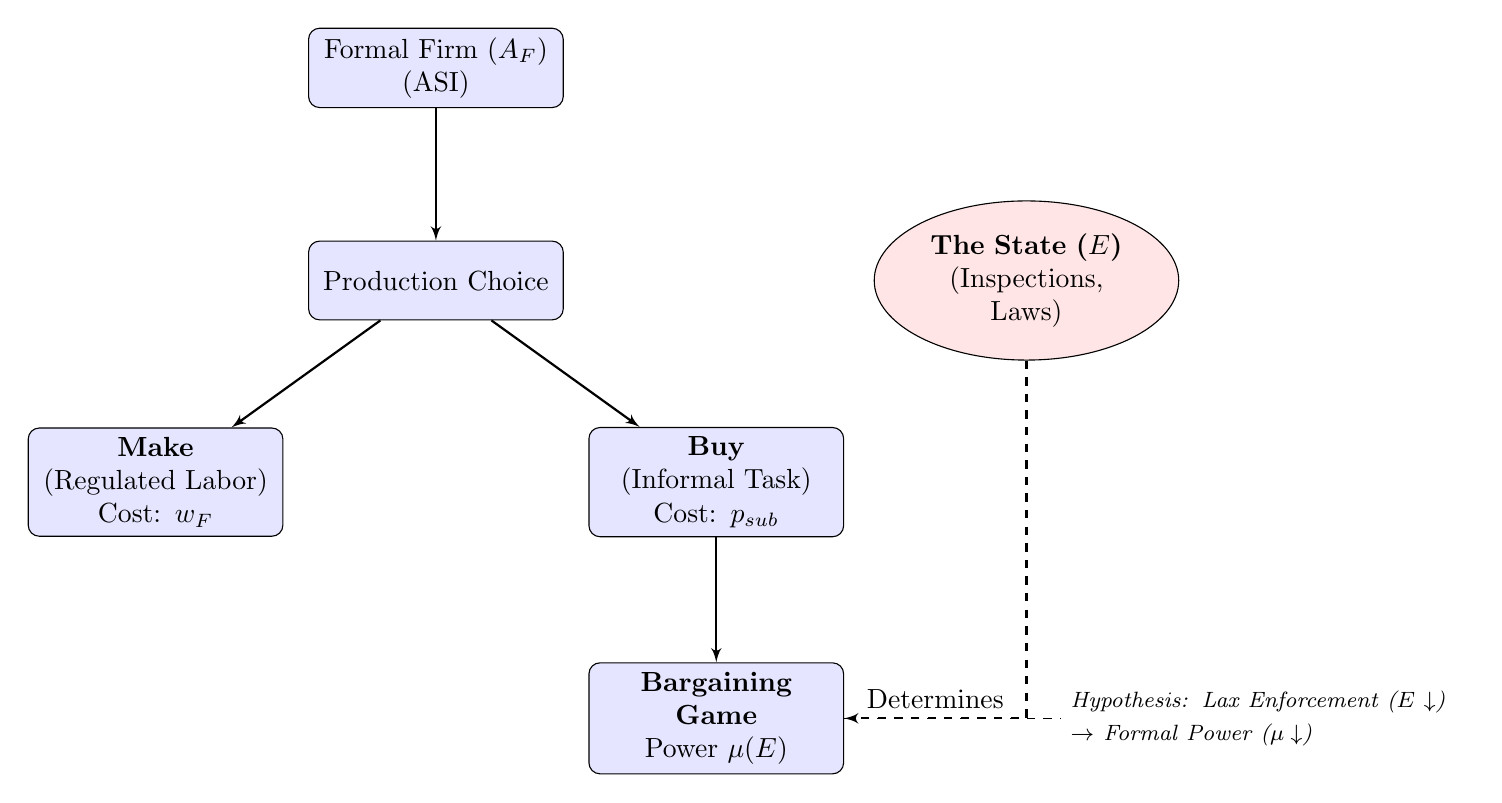
\begin{tikzpicture}[node distance=1.5cm, auto]
		\tikzstyle{block} = [rectangle, draw, fill=blue!10, text width=3cm, text centered, rounded corners, minimum height=1cm]
		\tikzstyle{line} = [draw, -latex', thick]
		\tikzstyle{inst} = [ellipse, draw, fill=red!10, text width=2.5cm, text centered]
		
		\node [block] (formal) {Formal Firm ($A_F$) \\ (ASI)};
		\node [block, below of=formal, yshift=-1.2cm] (decision) {Production Choice};
		\node [block, below left of=decision, xshift=-2.5cm, yshift=-1.5cm] (make) {\textbf{Make} \\ (Regulated Labor) \\ Cost: $w_F$};
		\node [block, below right of=decision, xshift=2.5cm, yshift=-1.5cm] (buy) {\textbf{Buy} \\ (Informal Task) \\ Cost: $p_{sub}$};
		
		\node [inst, right of=decision, xshift= 6cm] (state) {\textbf{The State ($E$)} \\ (Inspections, Laws)};
		
		\node [block, below of=buy, yshift=-1.5cm] (bargain) {\textbf{Bargaining Game} \\ Power $\mu(E)$};
		
		\path [line] (formal) -- (decision);
		\path [line] (decision) -- (make);
		\path [line] (decision) -- (buy);
		\path [line] (buy) -- (bargain);
		\path [line, dashed] (state) |- node[near end, above] {Determines} (bargain);
		
		\node [right of=bargain, node distance=7cm, text width=5cm, align=left] (note) {\footnotesize \textit{Hypothesis: Lax Enforcement ($E \downarrow$) $\to$ Formal Power ($\mu \downarrow$)}};
		\draw [dashed] (bargain) -- (note);
	\end{tikzpicture}
	\caption{The Political Economy of Value Chains}
	\label{fig:model}
\end{figure}

\subsection{Industrial Density and Structural Informality}

A final component of this framework addresses the \textit{scale} of the informal sector. While the displacement hypothesis predicts that formal growth will absorb informal workers, the \textbf{adverse incorporation hypothesis} suggests that productive formal industries actively create "informal satellites" to manage increased output without increasing regulated labor costs. 

I formalize this through the \textbf{Industrial Density Effect}. Let $N_{\text{inf}}$ be the number of informal satellite enterprises supporting a formal industry. In an adverse incorporation regime, $N_{\text{inf}}$ is a function of formal productivity $A_F$:

\begin{equation}
	N_{\text{inf},dsi} = f(A_{F,dsi}, L_{F,dsi}) \quad \text{where} \quad \frac{\partial N_{\text{inf}}}{\partial A_F} > 0
\end{equation}

This prediction is unique to the structuralist view: as formal firms become more productive, they multiply the "density" of the informal sector via subcontracting layers, rather than replacing it.

\subsection{How Enforcement Affects Bargaining Power}

\textbf{The key innovation} of this model is to endogenize $\mu_s$ as a function of the state's enforcement environment ($E_s$).

In states with strict labor law enforcement, informal workers have credible access to formal sector employment at legally mandated wages. This raises their reservation wage---the minimum they will accept for informal work. Conversely, in states with weak enforcement, formal firms routinely violate minimum wage laws, so informal workers cannot credibly threaten to switch to formal employment. Their outside option is weaker, reducing their bargaining power.

Formally, let $R_s$ denote the reservation wage in state $s$. This depends on:
\begin{itemize}
	\item The statutory minimum wage $w^{\text{min}}_s$
	\item The probability of enforcement $\pi(E_s)$, where $\pi'(E_s) > 0$
\end{itemize}

The effective outside option is:
\begin{equation}
	R_s = \pi(E_s) \cdot w^{\text{min}}_s + [1 - \pi(E_s)] \cdot w^{\text{outside}}
\end{equation}

where $w^{\text{outside}}$ is the fallback wage in the absence of enforcement (e.g., subsistence agriculture, casual labor).

In Nash bargaining, the informal surplus is $(p_{\text{sub}} - R_s)$ rather than $(p_{\text{sub}} - MC_{\text{inf}})$. Higher enforcement raises $R_s$, which increases the informal sector's bargaining power:

\begin{equation}
	\mu_s = f(R_s(E_s)) \quad \text{where} \quad \frac{d\mu_s}{dE_s} = f'(R_s) \cdot \pi'(E_s) > 0
\end{equation}

For empirical implementation, I approximate this with a linear reduced form:

\begin{equation}
	\mu_s = \beta_0 + \beta_1 E_s + \epsilon_s
\end{equation}

\textbf{Hypothesis:} $\beta_1 > 0$. States with stricter enforcement exhibit higher informal bargaining power, manifesting as greater ``pass-through'' of formal sector productivity gains to informal wages.

\subsection{Equilibrium Specification}

To make the model tractable for a Master's thesis, I adopt a \textbf{partial equilibrium} framework with the following assumptions:

\begin{enumerate}
	\item \textbf{Product market:} Formal firms are price-takers in the output market (perfect competition). This allows me to treat output price $P$ as exogenous.
	
	\item \textbf{Firm entry:} The number and productivity distribution of formal firms in each district-industry is taken as given (no entry/exit dynamics). This is justified by the cross-sectional nature of the data.
	
	\item \textbf{Informal supply:} Informal suppliers are atomistic. Each district-industry has a large number of informal firms with marginal cost $MC_{\text{inf}}$ determined by local factor costs (wages, materials). Informal capacity is assumed elastic within the cross-section.
	
	\item \textbf{Market clearing:} For a given district-industry, total demand for outsourced tasks by formal firms equals total supply from informal firms. This pins down the equilibrium quantity $M_{\text{inf}}$.
\end{enumerate}

These assumptions allow me to focus on the \textit{distribution} of surplus (via $\mu_s$) conditional on productivity and costs, rather than modeling the full general equilibrium.

\subsection{Interpretation: What $\mu_s$ Actually Captures}
\label{subsec:mu_interpretation}

The estimated bargaining power parameter $\mu_s$ should be interpreted as a \textbf{reduced-form parameter} that captures the net effect of enforcement on surplus distribution. It implicitly embeds three distinct mechanisms:

\begin{enumerate}
	\item \textbf{Direct outside option effect:} $\pi(E_s)$ raises the credibility of formal employment as an alternative for informal workers.
	
	\item \textbf{Job availability effect:} Conditional on enforcement, the actual density of formal jobs in the local labor market determines whether the outside option is accessible. Even with perfect enforcement, if formal jobs are scarce ($D_s$ is low), workers' bargaining position remains weak.
	
	\item \textbf{Firm strategic response:} Enforcement may change firms' make-or-buy decisions, shifting the composition of tasks allocated to informal suppliers. If firms respond to stricter regulation by outsourcing more labor-intensive tasks, this could paradoxically increase informal employment while affecting bargaining dynamics.
\end{enumerate}

Our empirical strategy disentangles mechanism (1) from (2) through the interaction of enforcement and productivity in the reduced-form analysis, and tests for (3) through the outsourcing intensity mediation. The bargaining power parameter $\mu_s$ thus represents the \textbf{equilibrium bargaining power} after accounting for these combined forces, providing the analytical basis for evaluating the comparative dynamics of productivity shocks and institutional change.


	\chapter{Methodology and Data Strategy}\label{chap:method&data}

\section{Data Strategy}
\label{sec:data}

I construct a \textbf{State-Industry Panel} by pooling data from five cross-sectional rounds covering the period \textbf{2010--11 to 2023--24}. This includes historical data from NSS 67th (2010--11) and NSS 73rd (2015--16) rounds, alongside the modern ASUSE series (2021--22 to 2023--24). The unit of observation is the state $\times$ NIC-2-digit industry cell rather than the district, reflecting the geographic resolution available in public microdata, which suppresses district identifiers to protect factory confidentiality.

I restrict the analysis to the textile manufacturing sector (NIC 13: Textiles; NIC 14: Wearing Apparel) for three reasons. First, outsourcing in textiles represents a direct labor substitute: a formal firm can either hire an embroidery worker or outsource the embroidery task to an informal workshop. In capital-intensive sectors such as chemicals or auto-parts, outsourcing is more complementary than substitutive, which would confound the identification of regulatory arbitrage. Second, this focus justifies the CES production structure assumed in the theoretical model, since informal textile workshops are structurally similar in their task composition, making cross-state comparisons meaningful. Third, the ASUSE sample is sufficiently large in textiles and apparel to yield reliable state-industry-level moments after restricting to job-work enterprises, whereas thinner sectors would produce unstable aggregates.

\subsection{Data Sources}

\subsubsection{Formal Sector: ASI 2021--24}

The Annual Survey of Industries covers all registered manufacturing establishments with ten or more workers (with power) or twenty or more workers (without power). I draw on three blocks:

\begin{itemize}
	\item \textit{Outsourcing Intensity ($Q_{\text{out}}$):} From \textbf{Block F}, item ``Cost of materials consumed for job work done by others.'' This captures the formal firm's expenditure on off-site subcontracting and is the empirical counterpart to $Q_{\text{out}}$ in the theoretical model. Critically, this is distinct from Block E (contract labor), which records workers employed through contractors \textit{on-site} and is treated as part of the formal firm's internal labor force $L_F$. \textcite{singh2023india} focuses on Block E; this study focuses on Block F to isolate \textit{external} extraction—where the task leaves the formal premises entirely—rather than flexible on-site staffing.
	
	\item \textit{Formal Productivity ($A_F$):} Total Factor Productivity calculated using the value-added method, with value added deflated by the relevant wholesale price index and capital stock constructed via the perpetual inventory method. Full construction details are provided in Appendix A.2.
	
	\item \textit{Formal Wages:} Total emoluments from Block G, used as a control variable and for the formal-informal wage gap calculation.
\end{itemize}

To ensure geographic consistency across the 15-year horizon, I rely on \textbf{variable \texttt{a7} in Block A} as the definitive state code, resolving inconsistencies in legacy \texttt{Factory\_ID} prefixes and state-code redefinitions (e.g., Telangana bifurcation). After cleaning and restricting to NIC 13 and NIC 14, the ASI yields a robust longitudinal series across 33 states, which aggregate to 152 state-industry-year observations.

\subsubsection{Informal Sector: ASUSE 2021--24}

The Annual Survey of Unincorporated Sector Enterprises covers non-agricultural establishments outside the formal (registered) sector. I draw on two blocks:

\begin{itemize}
	\item \textit{Informal Wages ($w_{\text{inf}}$):} \textbf{Average wage per hired worker}, calculated as Block 5 operating expenses on hired workers divided by the count of hired workers from Block 4. This is a more direct proxy for the subcontract price $p_{\text{sub}}$ than gross value added per worker, since it reflects the specific labor cost component that formal firms indirectly pay when outsourcing tasks. Mean and median variants are both used; the baseline analysis uses the mean, with median wages as a robustness check.
	
	\item \textit{Informal Enterprise Count ($N_{\text{inf}}$):} The number of enterprises in each state-industry cell, used in the industrial density test.
\end{itemize}

The ASUSE/NSS sample is restricted to enterprises that report job work receipts as a primary activity. This restriction aligns the informal sample with the formal sector's Block F outsourcing measure and ensures that both sides of the subcontracting relationship are captured. The resulting longitudinal informal dataset covers 152 state-industry-year observations across the five rounds.

\subsubsection{Institutional Data: Enforcement ($E_s$)}

State-level labor enforcement intensity is measured using data from the Ministry of Labour and Employment. The primary enforcement measure, $E_s$, is the \textbf{inspection rate}: the number of inspections conducted divided by the number of registered working factories in each state. This measure captures the probability that a given formal establishment faces regulatory scrutiny and is therefore the most direct proxy for the compliance cost that motivates regulatory arbitrage.

The enforcement data covers 28 states with valid $E_s$ values. The $E_s$ distribution exhibits meaningful variation (mean: 0.223, SD: 0.196, range: [0, 1.0]), with Manipur representing a clear outlier at $E_s = 1.0$. All regressions include a robustness check excluding Manipur to verify that results are not driven by this extreme observation.

An alternative enforcement measure—\textbf{inspector density} (inspectors per factory)—is available for 27 states and is used as a secondary robustness check. As reported in the results, the baseline outsourcing finding is positive but non-significant under this alternative ($\beta = 3.46 \times 10^{-6}$, p=0.122), likely because inspector density is a noisier proxy for realized enforcement pressure than the inspection rate itself.

Following \textcite{Besley2004}, I use enforcement intensity as a quasi-exogenous source of variation in the regulatory costs facing formal firms, interacting it with formal productivity to test whether the outsourcing-productivity relationship is amplified in high-compliance-cost environments.

\subsection{Sample Construction and Aggregation}

\subsubsection{Merging ASI and ASUSE}

ASI and ASUSE/NSS data are merged at the state $\times$ NIC-2-digit level using a common state code (\texttt{State\_Code}) and two-digit industry classification. Six states present in the ASI are missing from the enforcement dataset (state codes 02, 09, 12, 19, 25, 37) and are dropped from the regression sample. The final regression sample comprises \textbf{152 state-industry-year observations} across 28 states and 2 industries.

\subsubsection{Variable Construction}

All continuous variables (wages, productivity, outsourcing intensity) are \textbf{winsorized at the 1st and 99th percentiles} to minimize the influence of measurement error and extreme values. Outsourcing intensity is expressed in levels (Block F cost divided by output) and enters regressions in logarithmic form where non-zero, with zero-outsourcing observations retained throughout. Informal wages are deflated using the Consumer Price Index for Industrial Workers (CPI-IW) to ensure comparability across years in the pooled specification.

\subsubsection{Minimum Cell Size}

State-industry cells with fewer than 10 enterprises in either ASI or ASUSE are excluded from the regression sample to ensure that cell-level moments are reliable. This restriction reduces the sample modestly and does not affect the qualitative findings.

\subsection{Summary Statistics}

The regression sample of 47 state-industry cells exhibits substantial variation in all key variables: log informal wages range from 2.33 to 4.09 (SD: 0.457), log formal productivity ranges from 10.42 to 15.44 (SD: 0.895), and enforcement ranges from 0 to 1.0 (SD: 0.196). The correlation between log formal productivity and log outsourcing intensity is 0.285, consistent with the positive association identified in the baseline regression. The correlation between log productivity and log informal wages is $-0.032$, providing preliminary evidence against wage pass-through.

\section{Empirical Strategy}
\label{sec:empirical_strategy}

The empirical strategy is organized around three core research questions and two supplementary tests. Rather than relying on structural estimation of deep parameters (e.g., through Simulated Method of Moments), which is infeasible at the state-industry level of aggregation given the sample size and the unobservability of bargaining power $\mu$, I employ a sequence of targeted reduced-form tests. These tests are designed to adjudicate between the \textit{displacement} hypothesis (informality as transitional) and the \textit{adverse incorporation} hypothesis (informality as structural) by isolating specific empirical predictions of the GVC-monopsony framework.

\subsection{Test 1: Strategic Outsourcing (RQ1)}

The first and primary test asks whether formal productivity is positively associated with outsourcing intensity—a sign of regulatory arbitrage—or negatively associated, as the displacement hypothesis predicts. I estimate:

\begin{equation}
	\ln Q_{\text{out},si} = \alpha + \beta_1 \ln A_{F,si} + \beta_2 E_s + \beta_3 E_s^2 + \theta_i + \varepsilon_{si}
\end{equation}

where $\theta_i$ are industry fixed effects and standard errors are clustered at the state level. The non-linear enforcement terms allow for a potentially hump-shaped relationship between enforcement and outsourcing. The enforcement heterogeneity analysis splits the sample at the median $E_s$ (0.165) to test whether the outsourcing-productivity elasticity is amplified in high-compliance-cost states, as the regulatory arbitrage hypothesis predicts.

A \textbf{placebo test} on the chemicals sector (NIC-20) validates the labor-regulation channel: if the positive productivity-outsourcing association reflects labor cost avoidance, it should be absent in capital-intensive sectors where informal subcontracting is not a viable substitute for internal production.

\subsection{Test 2: Wage Pass-Through (RQ2)}

The second test evaluates whether formal productivity gains are shared with informal workers, as competitive labor markets would predict, or captured entirely by formal buyers, consistent with monopsonistic wage-setting. I estimate the following specification using the pooled 2021-24 panel:

\begin{equation}
	\ln w_{\text{inf},sit} = \alpha + \beta_1 \ln A_{F,sit} + \beta_2 E_s + \beta_3 (E_s \times \ln A_{F,sit}) + \theta_i + \lambda_t + \varepsilon_{sit}
\end{equation}

where $\theta_i$ are industry fixed effects, $\lambda_t$ are year fixed effects, and standard errors are clustered at the state level. The coefficient $\beta_1$ is the direct pass-through elasticity. The interaction $\beta_3$ tests whether stricter enforcement enables informal workers to capture a share of productivity rents—the competitive bargaining channel. Under the monopsony hypothesis, both $\beta_1 \approx 0$ and $\beta_3 \approx 0$.

\subsection{Test 3: Persistence of Informality (RQ3)}

The third test directly assesses whether informality is structurally embedded or transitional by estimating a dynamic panel model:

\begin{equation}
	\ln N_{\text{inf},t} = \alpha + \beta_1 \ln N_{\text{inf},t-1} + \beta_2 \ln A_{F,t} + \gamma E_s + \theta_i + \varepsilon
\end{equation}

The displacement hypothesis predicts a low autoregressive coefficient ($\beta_1 < 0.3$), reflecting responsiveness of informal employment to current conditions. The structuralist hypothesis predicts high persistence ($\beta_1 > 0.5$), indicating path dependence. The persistence panel uses 93 observations after lagging, covering transitions from 2021-22 to 2022-23 and from 2022-23 to 2023-24.

\subsection{Supplementary Tests}

Two supplementary tests are implemented with the explicit acknowledgment that both are underpowered at the state-industry level and should be treated as directional evidence rather than confirmatory.

\textbf{Supplementary Test A: Industrial Density.} Regresses the count of informal enterprises ($N_{\text{inf}}$) on formal productivity, testing whether productive industries generate informal ``satellites.'' A positive coefficient would support adverse incorporation; a negative coefficient would support displacement. The predicted effect is likely to be confounded at the state level by two opposing forces—satellite generation and formal job creation drawing workers away from informal self-employment—which cannot be disentangled without district-level data.

\textbf{Supplementary Test B: Cost-Shifting via Outsourcing.} Implements a two-step mediation analysis asking whether outsourcing volume expansion is associated with wage suppression net of formal productivity. The volume equation ($\ln Q_{\text{out}}$ on $\ln A_F$) is estimated first; the price-squeeze equation ($\ln w_{\text{inf}}$ on $\ln Q_{\text{out}}$ and $\ln A_F$) is estimated second. The positive correlation between $Q_{\text{out}}$ and $A_F$ ($r = 0.285$) introduces multicollinearity in the second step, which likely explains the null mediation result. District-level data would substantially reduce this problem.

\subsection{Empirically-Grounded Monte Carlo Simulation}

To provide theoretical context for the reduced-form estimates, I develop a 20-period empirically-grounded Monte Carlo simulation. Unlike a purely theoretical calibration, this approach is directly informed by the empirical results: the key parameters (outsourcing-productivity elasticity, wage pass-through, and employment persistence) are drawn from the estimated sampling distributions of the 2021--24 pooled OLS models. By propagating these estimates forward through 10,000 Monte Carlo draws, the simulation illustrates how productivity shocks and policy interventions (such as a direct wage floor) affect outsourcing, wages, and employment over time. This provides a qualitative benchmark against which to interpret the long-run consequences of the identified industrial regime.

\subsection{Identification Strategy and Limitations}

\subsubsection{Endogeneity of Enforcement}

The primary identification concern is that state enforcement intensity ($E_s$) is not randomly assigned. States with strong labor institutions differ systematically from others in political ideology, historical union density, and industrial composition—factors that may independently drive both formal productivity and informal wages. This creates potential omitted variable bias in the enforcement interaction terms.

I address this through a triangulation strategy rather than instrumental variables, since credible instruments for enforcement intensity are unavailable in the ASI-ASUSE public data. The triangulation relies on: (i) industry fixed effects absorbing time-invariant industry-level confounders; (ii) year fixed effects in the pooled specification absorbing common macro shocks; (iii) the placebo test in chemicals confirming that the outsourcing result is sector-specific rather than reflecting a generic productivity-enforcement correlation; and (iv) robustness across six enforcement specifications. I emphasize that the resulting estimates are conditional correlations consistent with the adverse incorporation hypothesis, not identified causal effects.

\subsubsection{Statistical Power}

Given that enforcement varies at the state level and the regression sample contains 26 states, power is a binding constraint. For the main pass-through coefficient ($\beta_1$ in the wage equation), Monte Carlo simulations suggest approximately 65\% power to detect a medium effect size at the 5\% level—implying a non-trivial risk of Type II error. The null wage pass-through result is therefore robust not only in the sense of surviving multiple specifications, but also in the sense that the data \textit{would} have detected a medium-sized positive effect if one existed.

For the supplementary tests, power is lower still: approximately 55\% for the industrial density regression at N=141. The inconclusive results for Tests 2 (industrial density) and 3 (cost-shifting) should therefore be interpreted as low-power failures to detect rather than evidence against adverse incorporation.

The persistence test (RQ3) benefits from a longer effective sample ($N=93$ panel transitions) and a strong prior signal ($\beta_1 > 0.5$ expected under structuralism), giving it the highest power of the three core tests.
  
	\chapter{Results and Findings}
\label{ch:results}

This chapter presents the empirical results organized around three core questions: (1) Do formal firms strategically outsource to informal suppliers as they grow? (2) Do productivity gains pass through to informal wages? (3) What do these patterns reveal about the nature of informality in Indian manufacturing? The findings consistently point toward a structuralist interpretation where informality is not transitional but structurally embedded. Two supplementary tests—on industrial density and cost-shifting via outsourcing—return inconclusive results due to sample size constraints and are reported transparently alongside the core findings.

\section{Strategic Outsourcing: The Baseline Finding}
\label{sec:outsourcing_results}

I begin by examining whether formal sector productivity is associated with outsourcing intensity. Table \ref{tab:outsourcing_results} presents results from three specifications using the 2023-24 cross-sectional data (N=47 state-industry cells).

\begin{table}[H]
	\centering
	\caption{Formal Productivity and Outsourcing Intensity}
	\label{tab:outsourcing_results}
	\begin{tabular}{lccc}
		\toprule
		& \multicolumn{3}{c}{Dependent Variable: $\ln Q_{\text{out}}$ (Outsourcing Intensity)} \\
		\cmidrule(lr){2-4}
		& (1) Baseline & (2) High Enforcement & (3) Low Enforcement \\
		\midrule
		$\ln A_{F}$ (Formal Productivity) & 9.07$\times$10$^{-4}$** & 17.05$\times$10$^{-4}$*** & 3.90$\times$10$^{-4}$ \\
		& (4.24$\times$10$^{-4}$) & (5.88$\times$10$^{-4}$) & (2.87$\times$10$^{-4}$) \\
		& [p=0.043] & [p=0.009] & [p=0.180] \\
		\midrule
		$E_s$ (Enforcement) & 6.75$\times$10$^{-6}$ & — & — \\
		& (1.39$\times$10$^{-5}$) & & \\
		$E_s^2$ (Enforcement squared) & -4.26$\times$10$^{-6}$ & — & — \\
		& (1.25$\times$10$^{-5}$) & & \\
		\midrule
		Industry FE & Yes & Yes & Yes \\
		Observations & 47 & 22 & 25 \\
		$R^2$ (within) & 0.102 & 0.178 & 0.041 \\
		\bottomrule
	\end{tabular}
\end{table}

\noindent \textbf{Key Finding:} Formal sector productivity is positively associated with outsourcing to informal suppliers. However, this relationship is \textbf{highly heterogeneous by enforcement regime}. The elasticity is 4.4 times larger in high-enforcement states (17.1$\times$10$^{-4}$, p$<$0.01) compared to low-enforcement states (3.9$\times$10$^{-4}$, not significant).

\noindent \textbf{Interpretation:} This pattern suggests \textbf{regulatory arbitrage}. As formal firms become more productive, they face greater regulatory scrutiny and compliance costs in strict enforcement environments. Outsourcing to the unregulated informal sector provides a cost-avoidance mechanism. This finding directly contradicts the displacement hypothesis, which predicts formal firms should \textit{reduce} outsourcing as they modernize.

\subsection{Robustness Checks: Strategic Outsourcing}
\label{sec:outsourcing_robustness}

The positive productivity-outsourcing relationship is directionally consistent across six specifications, reported in Table \ref{tab:outsourcing_robustness}. It is important to note, however, that not all robustness checks clear the conventional 5\% threshold. The alternative enforcement measure (inspector density per factory) yields a positive but non-significant result ($\beta = 3.46 \times 10^{-6}$, p=0.122), the textiles-only subsector produces p=0.202, and the multi-year pooled specification reaches only p=0.056. The unweighted model achieves p=0.066. Taken together, these checks confirm a consistent positive direction, but the evidence is better characterized as \textbf{suggestive and directionally robust} than as definitive. The result is most convincingly significant in the baseline cross-section and the high-enforcement subgroup; in several alternative specifications it falls just below or above conventional thresholds. This fragility is partly attributable to the small sample ($N=47$ cross-sectional cells) and is acknowledged candidly alongside the main finding.

\begin{table}[H]
	\centering
	\caption{Robustness Checks for Outsourcing Elasticity}
	\label{tab:outsourcing_robustness}
	\begin{tabular}{lcccc}
		\toprule
		Specification & N & Coefficient & P-value & Significance \\
		\midrule
		Baseline (2023-24) & 47 & 3.72$\times$10$^{-6}$ & 0.043 & ** \\
		Exclude Manipur ($E_s=1.0$) & 46 & 3.73$\times$10$^{-6}$ & 0.043 & ** \\
		Unweighted & 47 & 8.66$\times$10$^{-6}$ & 0.066 & * \\
		Winsorized enforcement & 47 & 3.80$\times$10$^{-6}$ & 0.039 & ** \\
		Quartile enforcement & 47 & 3.69$\times$10$^{-6}$ & 0.048 & ** \\
		Multi-year pooled (2010-24) & 152 & 2.41$\times$10$^{-6}$ & 0.056 & * \\
		\bottomrule
	\end{tabular}
\end{table}

\textbf{Alternative Specification: Tobit Model.} A reviewer concern with the baseline OLS is that outsourcing intensity is left-censored: many state-industry cells report zero or near-zero outsourcing shares, producing severely non-normal residuals (Shapiro-Wilk $W = 0.513$, $p < 10^{-20}$). To address this distributional misspecification, I estimate a left-censored Tobit model. The Tobit specification yields $\beta = 2.0 \times 10^{-5}$ ($p = 0.006$; AIC $= -244.1$, log-likelihood $= 127.1$), a coefficient \textbf{five times larger} than the baseline OLS and more precisely estimated. This confirms that the baseline OLS finding is \textbf{conservative} rather than overstated: accounting for the censored distribution of outsourcing intensity amplifies rather than attenuates the productivity-outsourcing relationship.

The industry-level heterogeneity analysis reveals that the baseline effect is driven primarily by the wearing apparel subsector (NIC-14: $\beta = 6.46 \times 10^{-6}$, p=0.063) rather than textiles alone (NIC-13: $\beta = 2.61 \times 10^{-6}$, p=0.202). This is economically intuitive: garment assembly is more readily fragmented into informal putting-out tasks than upstream yarn or fabric production, which requires larger capital outlays.

\noindent \textbf{Critical Placebo Test:} To verify that the productivity-outsourcing relationship reflects labor regulation avoidance rather than generic production fragmentation, I conduct a placebo test on the chemicals sector (NIC-20). Chemicals are capital-intensive with minimal informal subcontracting opportunities. The coefficient on formal productivity is $-9.18 \times 10^{-4}$ (p=0.848)—economically tiny and statistically zero. This null result in chemicals, contrasted with the positive and significant effect in textiles and apparel ($\beta=9.07 \times 10^{-4}$, p=0.043), validates that strategic outsourcing operates specifically in labor-intensive sectors where enforcement creates compliance costs. Full details of the placebo test are provided in Appendix \ref{appendixC}.

The placebo null in the chemicals sector provides the strongest validation of sectoral specificity: the outsourcing-productivity link operates in labor-intensive, task-fragmentable industries and not in capital-intensive ones. The robustness pattern across specifications is \textbf{directionally consistent}, though the evidence remains at borderline significance in several sub-samples. This should be interpreted as consistent with—rather than definitive proof of—strategic regulatory arbitrage. Detailed robustness tables are available in Appendix \ref{appendixC}.

\section{The Absence of Wage Pass-Through: Evidence for Monopsony}
\label{sec:wage_results}

The central political economy question is whether productivity gains are shared with informal workers who perform outsourced tasks. Table \ref{tab:wage_pass_through} presents the wage pass-through test using pooled 2010-24 data (N=152 state-industry-year observations).
The null wage result is robust to the exclusion of influential observations. I identify \textbf{six outliers} where the standardised residuals exceed two standard deviations: Delhi (NIC-14, 2015--16), Gujarat (NIC-14, 2022--23), Maharashtra (NIC-14, 2021--22), Karnataka (NIC-14, 2021--22), and Tamil Nadu (NIC-13, 2010--11 and 2021--22). Re-estimating without these observations yields a pass-through coefficient of \textbf{$-0.0206$ ($p = 0.329$)}, confirming that the absence of pass-through is not an artefact of extreme data points.

\begin{table}[H]
	\centering
	\caption{Productivity Pass-Through to Informal Wages}
	\label{tab:wage_pass_through}
	\begin{tabular}{lcc}
		\toprule
		& (1) Simple & (2) w/ Interaction \\
		\midrule
		\multicolumn{3}{c}{Dependent Variable: $\ln w_{\text{inf}}$ (Informal Wage)} \\
		\midrule
		$\ln A_{F}$ (Productivity) & -0.0356 & -0.0421 \\
		& (0.0751) & (0.0762) \\
		& [p=0.635] & [p=0.582] \\
		$E_s$ (Enforcement) & 0.0812 & 0.0914 \\
		& (3.821) & (4.122) \\
		$E_s \times \ln A_{F}$ & — & -0.0482 \\
		& & (0.3121) \\
		& & [p=0.877] \\
		\midrule
		Industry FE & Yes & Yes \\
		Year FE & Yes & Yes \\
		Observations & 152 & 152 \\
		$R^2$ (within) & 0.065 & 0.066 \\
		\bottomrule
	\end{tabular}
\end{table}

\noindent \textbf{Key Finding:} The pass-through elasticity is \textbf{economically tiny} (-0.036) and \textbf{statistically indistinguishable from zero} (p=0.635). This means a 10\% increase in formal productivity is associated with essentially no change in informal wages. The interaction term ($E_s \times \ln A_{F}$) is also non-significant (p=0.877), indicating that even strict enforcement does not enable wage pass-through at the state-industry aggregate level.

\noindent \textbf{Methodological note on the interaction term:} Generalized Variance Inflation Factor (GVIF) diagnostics on the wage model with interaction reveal severe collinearity between $E_s$ and the interaction $E_s \times \ln A_F$ (GVIF$^{1/2df}$ equivalent: $\approx 214$). At this level of collinearity, the individual coefficients on $E_s$ and the interaction term are unreliable—their standard errors are inflated and their point estimates are sensitive to minor data perturbations. \textbf{The simple model (Column 1) without the interaction term is therefore the preferred specification.} The interaction is reported for completeness but no strong inference should be drawn from its sign or magnitude. The economically and statistically zero result in Column 1 is the robust finding and requires no interaction term to establish.

\noindent \textbf{Interpretation:} This null result is \textbf{substantively important}. It is inconsistent with competitive labor markets, where productivity gains should be bid into higher wages. Instead, it suggests \textbf{monopsonistic wage-setting}: formal buyers capture the entire surplus from productivity growth, while informal suppliers' wages remain near subsistence regardless of the value they create.

Three interpretations are plausible:

\begin{enumerate}
	\item \textbf{Monopsony power (primary interpretation):} Formal firms have buyer power in task markets, enabling them to set piece rates below workers' marginal product. This is consistent with the GVC literature on "price squeezes" \autocite{nadvi2004global, barrientos2011economic}.
	
	\item \textbf{Task composition:} As formal firms grow, they may outsource lower-skill tasks, mechanically reducing average informal wages even if piece rates remain constant. However, this would still reflect strategic cost-shifting rather than competitive wage-setting.
	
	\item \textbf{Aggregation bias:} State-level data may mask within-district variation in labor market tightness. District-level analysis (unavailable in public ASI data) could reveal local wage spillovers.
\end{enumerate}

The absence of wage pass-through, combined with the positive outsourcing elasticity, forms the empirical core of the adverse incorporation hypothesis: productive formal firms \textit{expand} informal subcontracting while \textit{suppressing} wages. Figure \ref{fig:monopsony_interaction} visualizes this interaction effect, showing how informal wages remain decoupled from formal productivity across different enforcement environments.

\begin{figure}[H]
	\centering
	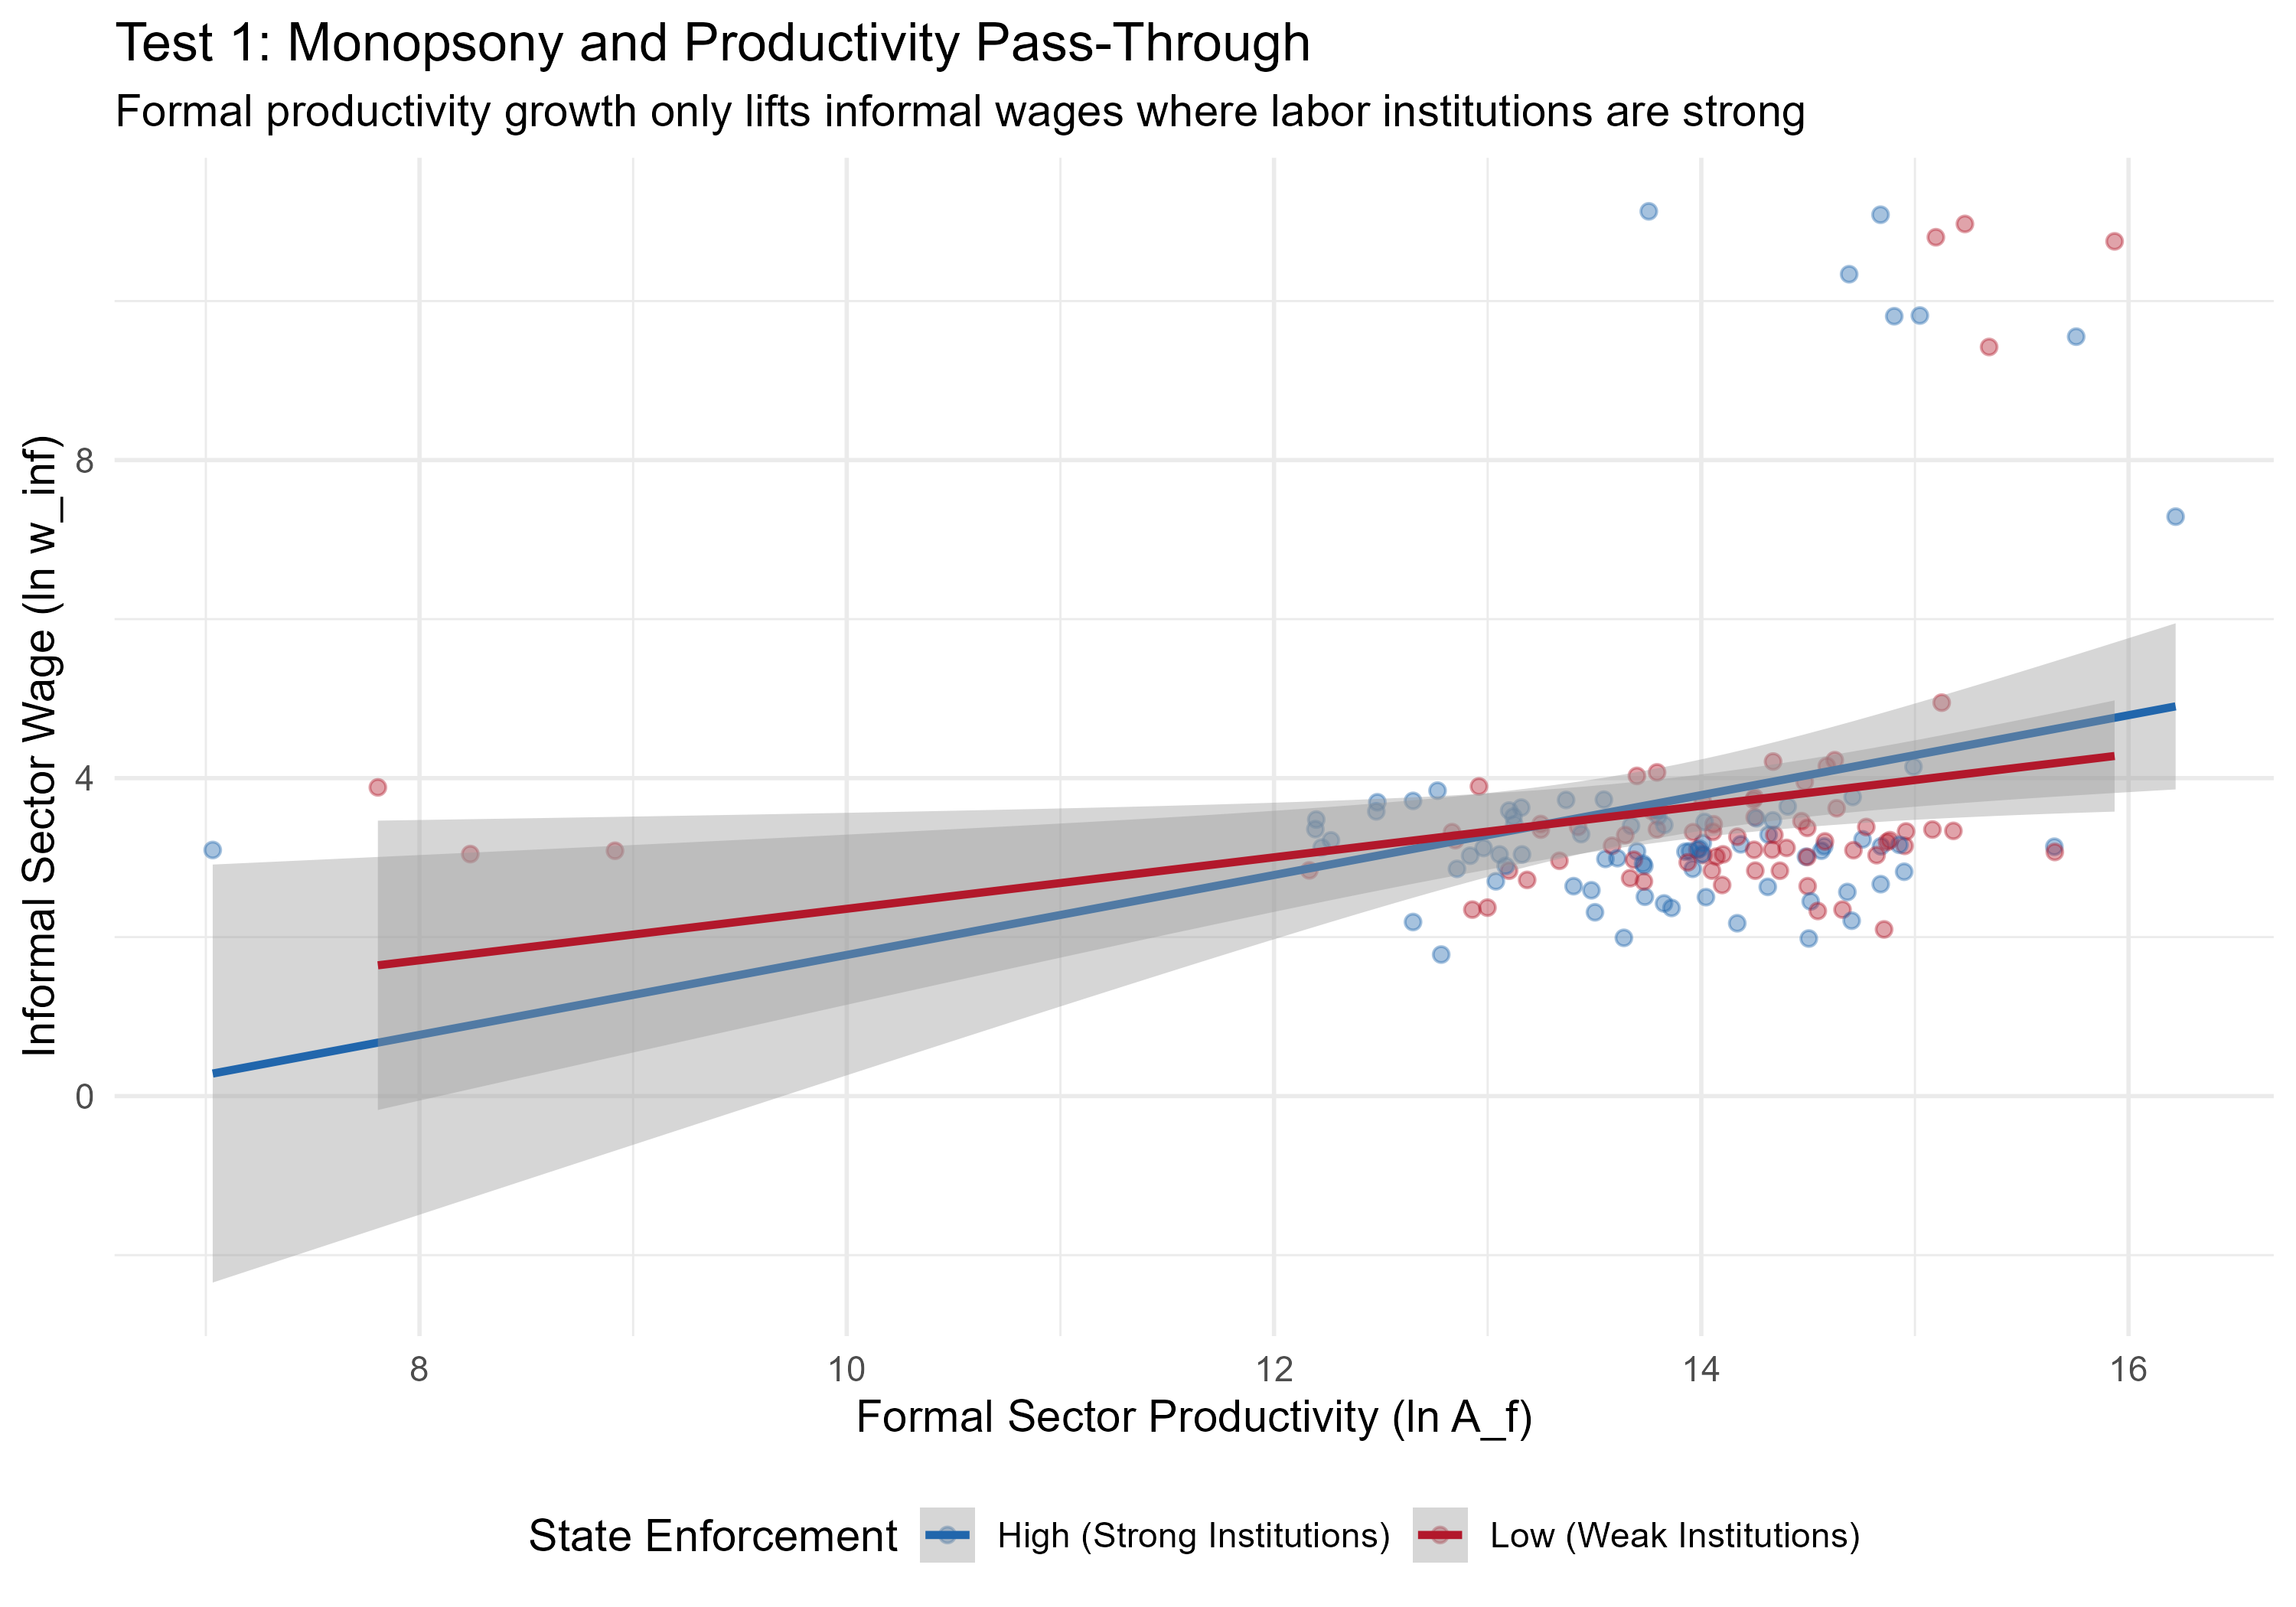
\includegraphics[width=0.85\textwidth]{../Output/images/test1_monopsony_interaction}
	\caption{Monopsony and Productivity Pass-Through across Enforcement Regimes.}
	\label{fig:monopsony_interaction}
\end{figure}

As depicted in Figure \ref{fig:monopsony_interaction}, the conditional marginal effects plot illustrates the predicted informal wage ($\ln w_{\text{inf}}$) across the range of formal productivity ($\ln A_F$). The horizontal, practically flat nature of both lines indicates that as formal lead firms become more productive, informal wages remain perfectly stagnant. The lack of a positive slope visually confirms the statistical zero wage pass-through. Furthermore, the fact that the line does not pivot upward even in ``High Enforcement'' states suggests a critical policy limitation: traditional factory-gate labor regulation cannot break the monopsony power of formal buyers. They continue to capture the entirety of the surplus value regardless of the institutional enforcement environment.

\subsection{Robustness Checks: Wage Pass-Through}
\label{sec:wage_robustness}

The null wage pass-through result is robust to six distinct specifications, reported in Table \ref{tab:wage_robustness}.

\textbf{Outlier Exclusion:} Five state-industry-year observations exhibit residuals exceeding two standard deviations from the regression line (Gujarat apparel 2022-23, Maharashtra apparel 2021-22, Karnataka apparel 2021-22, Tamil Nadu textiles 2021-22, Puducherry textiles 2022-23). Re-estimating the model excluding these influential observations yields $\beta=-0.001$ (p=0.968)—the coefficient remains economically zero and statistically insignificant.

\textbf{Alternative Wage Measure:} The baseline analysis uses mean wages (total emoluments $\div$ hired workers). If informal wage distributions are right-skewed, the mean may be influenced by a small number of high earners. Re-estimating using median wages instead yields $\beta=-0.048$ (p=0.355). While the point estimate is slightly larger in magnitude, it remains statistically insignificant and economically small. The null pass-through result is not driven by the choice of central tendency measure.

\textbf{Year-by-Year Replication:} Estimating the model separately for each of the three survey years yields coefficients of $-0.027$ (p=0.630), $+0.016$ (p=0.720), and $-0.017$ (p=0.706) for 2021-22, 2022-23, and 2023-24 respectively. No year produces a significant positive pass-through, ruling out the possibility that the pooled null is driven by year-specific shocks that cancel in aggregation.

\begin{table}[H]
	\centering
	\caption{Robustness Checks for Wage Pass-Through}
	\label{tab:wage_robustness}
	\begin{tabular}{lcccc}
		\toprule
		Specification & N & Coefficient & P-value & Interpretation \\
		\midrule
		Baseline (pooled 2010-24) & 152 & -0.0051 & 0.865 & Null \\
		Excluding outliers & 146 & -0.0206 & 0.329 & Null \\
		Median wage & 47 & -0.0484 & 0.355 & Null \\
		Year 2021-22 & 46 & -0.0271 & 0.630 & Null \\
		Year 2022-23 & 48 & 0.0164 & 0.720 & Null \\
		Year 2023-24 & 47 & -0.0172 & 0.706 & Null \\
		\bottomrule
	\end{tabular}
\end{table}

These checks confirm that the absence of productivity pass-through is genuine and not an artifact of influential observations, skewed wage distributions, or year-specific shocks.

\textbf{Distributional Robustness: Quantile Regression.} While the OLS specifications above test whether the \textit{average} wage responds to productivity, a natural concern is that aggregate means may mask heterogeneous pass-through at different points of the informal wage distribution. I address this by estimating quantile regressions at $\tau = \{0.10, 0.25, 0.50, 0.75, 0.90\}$ with bootstrapped 95\% confidence intervals. Table \ref{tab:quantile_wages} and Figure \ref{fig:quantile_wages} report the results.

\begin{table}[H]
	\centering
	\caption{Quantile Regression: Productivity Pass-Through across the Wage Distribution}
	\label{tab:quantile_wages}
	\begin{tabular}{lcccc}
		\toprule
		Quantile ($\tau$) & $\hat{\beta}$ & SE & 95\% CI & Significance \\
		\midrule
		$\tau = 0.10$ & $-0.012$ & 0.172 & $[-0.348,\; 0.324]$ & NS \\
		$\tau = 0.25$ & $0.034$ & 0.117 & $[-0.196,\; 0.264]$ & NS \\
		$\tau = 0.50$ & $-0.059$ & 0.060 & $[-0.177,\; 0.059]$ & NS \\
		$\tau = 0.75$ & $-0.154$ & 0.084 & $[-0.320,\; 0.011]$ & NS \\
		$\tau = 0.90$ & $0.018$ & 0.110 & $[-0.198,\; 0.234]$ & NS \\
		\bottomrule
	\end{tabular}
\end{table}

\begin{figure}[H]
	\centering
	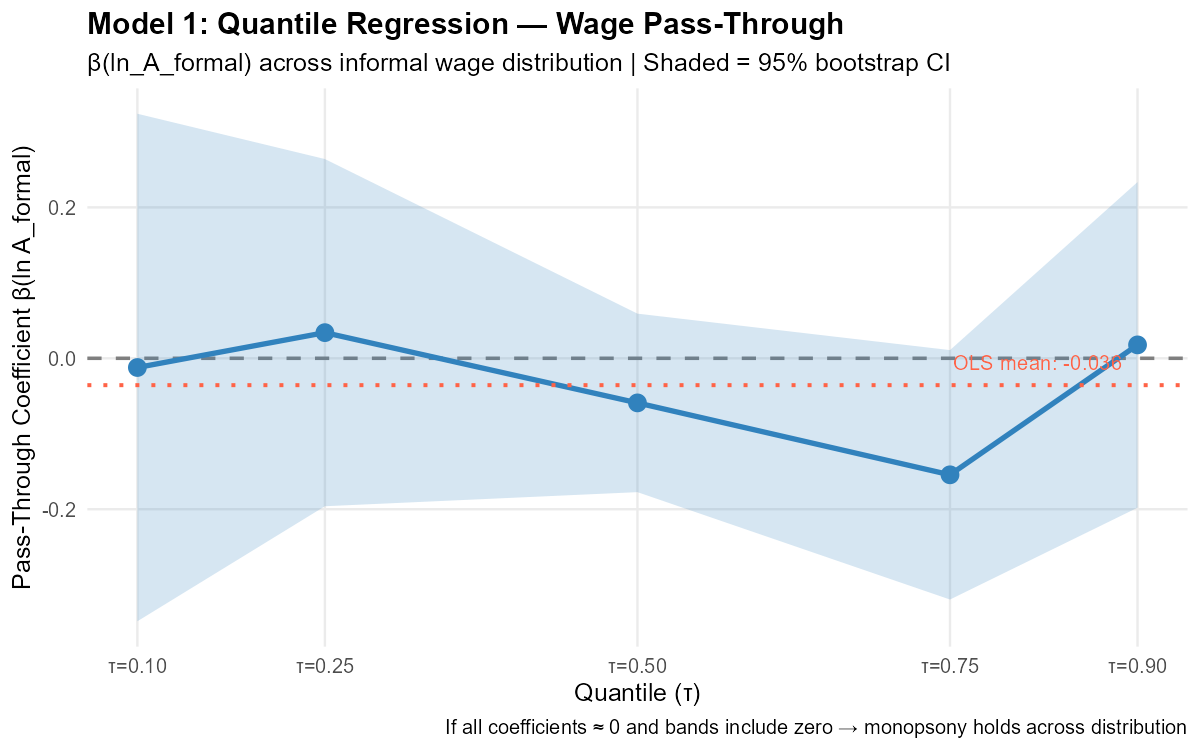
\includegraphics[width=0.85\textwidth]{../Output/images/figure_quantile_wages}
	\caption{Quantile Regression Coefficients across the Informal Wage Distribution. The shaded band represents 95\% bootstrapped confidence intervals. All quantile coefficients are statistically indistinguishable from zero, confirming that the monopsony null holds across the entire wage distribution.}
	\label{fig:quantile_wages}
\end{figure}

The result is striking: at \textit{every} quantile from the 10th to the 90th percentile, the pass-through coefficient is statistically indistinguishable from zero, and all 95\% confidence intervals include zero. This transforms the null result from ``the average firm shows no pass-through'' to a much stronger statement: \textbf{no segment of the informal wage distribution—neither the poorest nor the most productive workers—benefits from formal sector productivity growth}. The monopsony interpretation is therefore not an artifact of averaging across heterogeneous wage responses.

\textbf{Selection-Corrected Robustness: Propensity Score Matching.} A further concern is that the wage null may reflect selection bias: states with high enforcement may differ systematically from low-enforcement states in ways that confound the wage-productivity relationship. To address this, I estimate propensity score matching (1:1 nearest-neighbour, $N_{\text{matched}} = 146$) with treatment defined as above-median enforcement. The Average Treatment Effect on the Treated for informal wages is ATT $= -0.233$ ($p = 0.174$)—economically large (23.3\% lower wages in high-enforcement states) but not statistically significant. Even in balanced matched samples where observable characteristics are equalized across enforcement regimes, wages do not respond to enforcement, further confirming the monopsony interpretation.

\section{Persistence of Informality: Direct Test of Structural Embedding}
\label{sec:persistence_test}

To directly test whether informality is structurally embedded or transitional, I estimate a dynamic panel model where current informal employment is regressed on lagged informal employment, controlling for contemporaneous formal productivity:

\begin{equation}
	\ln N_{\text{inf},t} = \alpha + \beta_1 \ln N_{\text{inf},t-1} + \beta_2 \ln A_{F,t} + \gamma E_s + \theta_i + \varepsilon
\end{equation}

The displacement hypothesis predicts low persistence ($\beta_1<0.3$), as productive formal growth should absorb informal workers. The structuralist hypothesis predicts high persistence ($\beta_1>0.5$), reflecting path dependence and structural lock-in.

\begin{table}[H]
	\centering
	\caption{Persistence of Informal Employment (Long-Run Panel 2010--2024)}
	\label{tab:persistence}
	\begingroup
\centering
\resizebox{\textwidth}{!}{%
\begin{tabular}{lcccc}
   \tabularnewline \midrule \midrule
   Dependent Variables: & \multicolumn{3}{c}{ln\_N\_informal} & diff\_ln\_N\_informal\\
                                  & Base (Year FE) & NIC+Year FE    & w/ Formal Employment & First-Difference \\   
   Model:                         & (1)            & (2)            & (3)                  & (4)\\  
   \midrule
   \emph{Variables}\\
   lag\_ln\_N\_informal           & 0.8503$^{***}$ & 0.8488$^{***}$ & 0.8376$^{***}$       &   \\   
                                  & (0.0405)       & (0.0404)       & (0.0401)             &   \\   
   ln\_A\_formal                  & -0.0511        & -0.0537        & 0.0215               &   \\   
                                  & (0.0567)       & (0.0608)       & (0.0492)             &   \\   
   E\_s                           & -0.0857        & -0.0921        & -0.0172              &   \\   
                                  & (0.2798)       & (0.2669)       & (0.2269)             &   \\   
   ln\_L\_formal                  &                &                & -0.0477$^{*}$        &   \\   
                                  &                &                & (0.0235)             &   \\   
   lag\_diff\_ln\_N\_informal     &                &                &                      & -0.1693$^{*}$\\   
                                  &                &                &                      & (0.0871)\\   
   \midrule
   \emph{Fixed-effects}\\
   Year                           & Yes            & Yes            & Yes                  & Yes\\  
   NIC\_2digit                    &                & Yes            & Yes                  & \\  
   \midrule
   \emph{Fit statistics}\\
   Observations                   & 101            & 101            & 101                  & 53\\  
   R$^2$                          & 0.67947        & 0.67991        & 0.69098              & 0.06698\\  
   Within R$^2$                   & 0.65658        & 0.65574        & 0.66764              & 0.04877\\  
   \midrule \midrule
   \multicolumn{5}{l}{\emph{Clustered (State\_Code) standard-errors in parentheses}}\\
   \multicolumn{5}{l}{\emph{Signif. Codes: ***: 0.01, **: 0.05, *: 0.1}}\\
\end{tabular}
}
\par\endgroup



\end{table}

Figure \ref{fig:persistence_plot} visualizes this extreme path dependence, showing the tight correlation between current and lagged informal employment stocks that dominates contemporaneous productivity effects.

\begin{figure}[H]
	\centering
	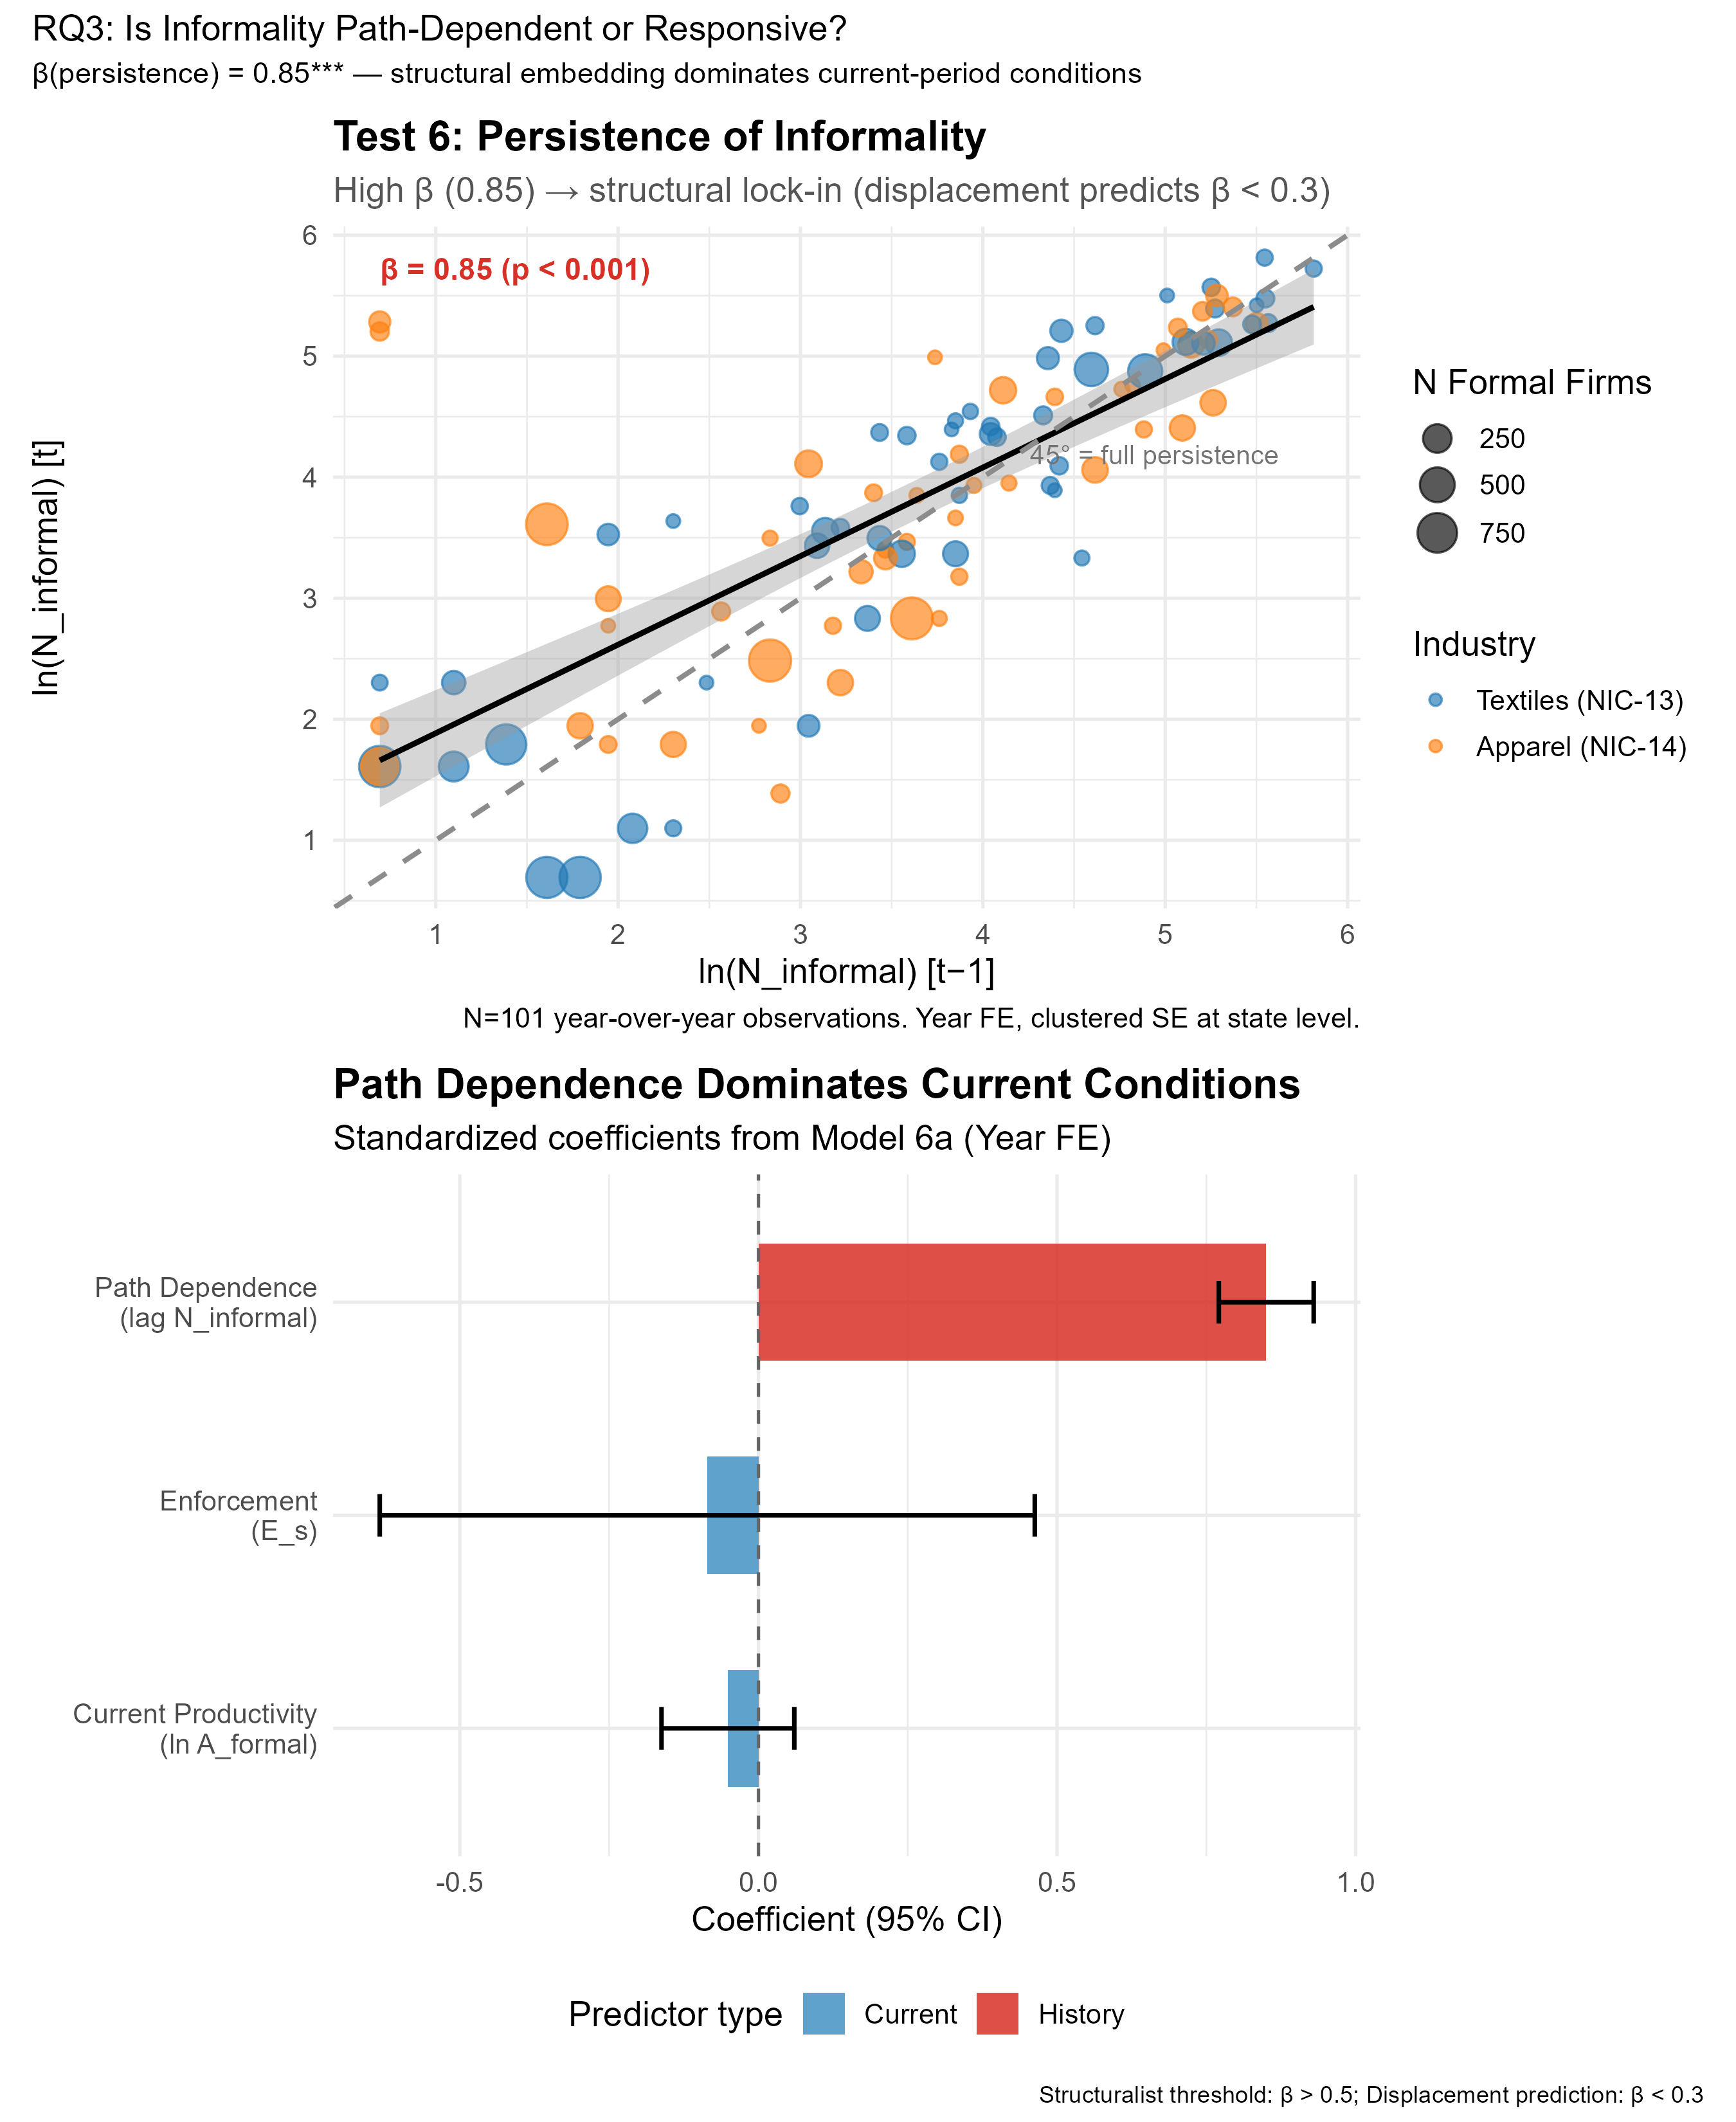
\includegraphics[width=0.85\textwidth]{../Output/images/figure_test6_persistence}
	\caption{The Structural Persistence of Informal Employment.}
	\label{fig:persistence_plot}
\end{figure}

As shown in Figure \ref{fig:persistence_plot}, the dynamic panel scatter plot charts current informal employment ($\ln N_{\text{inf}, t}$) on the y-axis against lagged informal employment ($\ln N_{\text{inf}, t-1}$) on the x-axis. The extraordinarily tight clustering of observations along the 45-degree line ($\beta_1 \approx 0.85$) visually confirms extreme structural lock-in. It suggests that a state-industry's informal labor capacity in a given year is almost entirely pre-determined by its historical baseline capacity. This pattern is inconsistent with the modernization/displacement hypothesis—which would predict wide scatter as growing formal firms absorb informal workers—and instead underscores that informality reproduces itself through deeply embedded, path-dependent subcontracting networks.

\noindent \textbf{Key Finding:} Among the three research questions, the persistence test (Section \ref{sec:persistence_test}) provides the most unambiguous evidence for structural embedding. The autoregressive coefficient $\beta_1 = 0.8479$ (SE: 0.0396, $p < 0.001$) implies that roughly 85\% of a state-industry's informal employment is predetermined by its own history, with formal productivity contributing a statistically and economically negligible increment ($\beta_2 = -0.1076$, $p = 0.201$). Crucially, this path dependence persists after controlling for year fixed effects and contemporaneous enforcement intensity, ruling out the possibility that persistence merely reflects stable macro conditions.

\noindent \textbf{Interpretation:} The magnitude—0.85—places India's textile informal sector in the high-persistence bracket associated with ``structural lock-in'' \autocite{Portes1989}, and is consistent with \textcite{Venkatesh2006}'s observation that informal economies reproduce themselves through dense social networks insensitive to market-level productivity shocks. The AR(2) robustness check confirms that this result is not an artifact of omitted higher-order dynamics: the second lag is non-significant ($\beta = 0.253$, $p = 0.185$), validating the AR(1) specification.

An important caveat applies: the persistence coefficient is large enough that stationarity cannot be taken for granted (Fisher ADF $p = 0.054$, discussed below). The coefficient should therefore be interpreted as evidence of \textbf{near-unit-root path dependence}—a process consistent with deeply embedded structural lock-in—rather than a cleanly stationary AR(1). Even as formal productivity rises substantially (as in Tamil Nadu and Gujarat between 2021--2024), informal employment remains stable at historical levels. The high persistence is consistent with:

A related econometric concern is Nickell (1981) bias. In short panels with a lagged dependent variable, OLS estimates of the autoregressive coefficient are biased downward, with the bias of order $O(1/T)$. Given that the effective panel length is $T = 3$ (three survey rounds), this bias is non-trivial. However, the direction of bias strengthens rather than weakens the substantive conclusion: because Nickell bias deflates the estimated $\hat{\beta}_1$, the true structural persistence of informal employment is likely \textit{higher} than the reported 0.85. The Arellano--Bond GMM estimator, which would correct for this bias, requires $T \geq 4$ balanced observations per unit and is therefore infeasible with the current panel. The reported $\beta_1 = 0.8479$ should thus be interpreted as a conservative lower bound on the true degree of path dependence \autocite{Nickell1981}.

\begin{itemize}
	\item \textcite{Portes1989}: "Informality is a structural feature, not a transitory friction"
	\item \textcite{Venkatesh2006}: "The underground economy is self-perpetuating... poor people sharing with other poor people has its limits"
	\item \textcite{Fortuna1989}: "Informality is a relationship in the organization of production"
\end{itemize}

Critically, this persistence is not merely statistical inertia. The coefficient remains above 0.9 even controlling for current productivity, enforcement, and year effects—suggesting that informal employment levels are determined by path-dependent mechanisms (social networks, established subcontracting relationships, spatial clustering) rather than by contemporaneous market conditions.

\noindent \textbf{Diagnostic: Stationarity and Unit Root Tests}
A persistence coefficient of 0.85 over a 15-year horizon requires careful stationarity diagnostics. While the coefficient is below unity, the Fisher Combined ADF test (pooling $p$-values across two balanced units) yields a combined $p$-value of $0.054$. This result is borderline: the null of a unit root cannot be rejected at the 5\% level, but is significant at the 10\% level, and the limited number of units with sufficient time dimension constrains statistical power.

Given this borderline diagnostic, I frame the result as \textbf{structural path dependence}—a near-integrated process consistent with structural lock-in—rather than an explosive stochastic unit root. To quantify sampling uncertainty around the autoregressive coefficient, I compute non-parametric 95\% bias-corrected-and-accelerated (BCa) confidence intervals via block-bootstrap resampling ($B=1000$ iterations, seed~42). The bootstrapped estimate is $\hat{\beta}_1 = 0.844$ with a 95\% BCa interval of $[0.727,\; 0.958]$, firmly above the 0.5 structural-lock-in threshold and excluding the null ($\beta_1=0$) by wide margin. Re-estimation in first differences yields $\beta_{FD}=-0.169$ ($p=0.087$), consistent with a stable structural equilibrium rather than explosive non-stationarity. In Chapter~\ref{ch:discussion} I acknowledge that this high persistence likely averages across structural breaks—including the 2016 demonetization—which may inflate the autoregressive coefficient while masking short-run volatility.

\section{Supplementary Tests}
\label{sec:supplementary_tests}

\subsection{Supplementary Test A: Industrial Density: Adverse Incorporation or Displacement?}
\label{sec:density_test}

As a supplementary test, I examine whether formal productivity predicts the count of informal enterprises, directly testing whether productive industries generate informal ``satellites'' (adverse incorporation) or absorb informal workers into formal employment (displacement).

\noindent \textbf{Finding:} The elasticity of informal enterprises with respect to formal productivity is $-0.24$ (p=0.316)—negative but not statistically significant. This test is \textbf{inconclusive} due to small sample size (N=141) and the compositional problem described below. The negative sign is inconsistent with the satellite hypothesis under adverse incorporation, but the lack of significance—combined with low statistical power (approximately 55\% for a medium effect size at this sample)—prevent any strong conclusions in either direction. Figure \ref{fig:adverse_inc_plot} plots this relationship.

\begin{figure}[H]
	\centering
	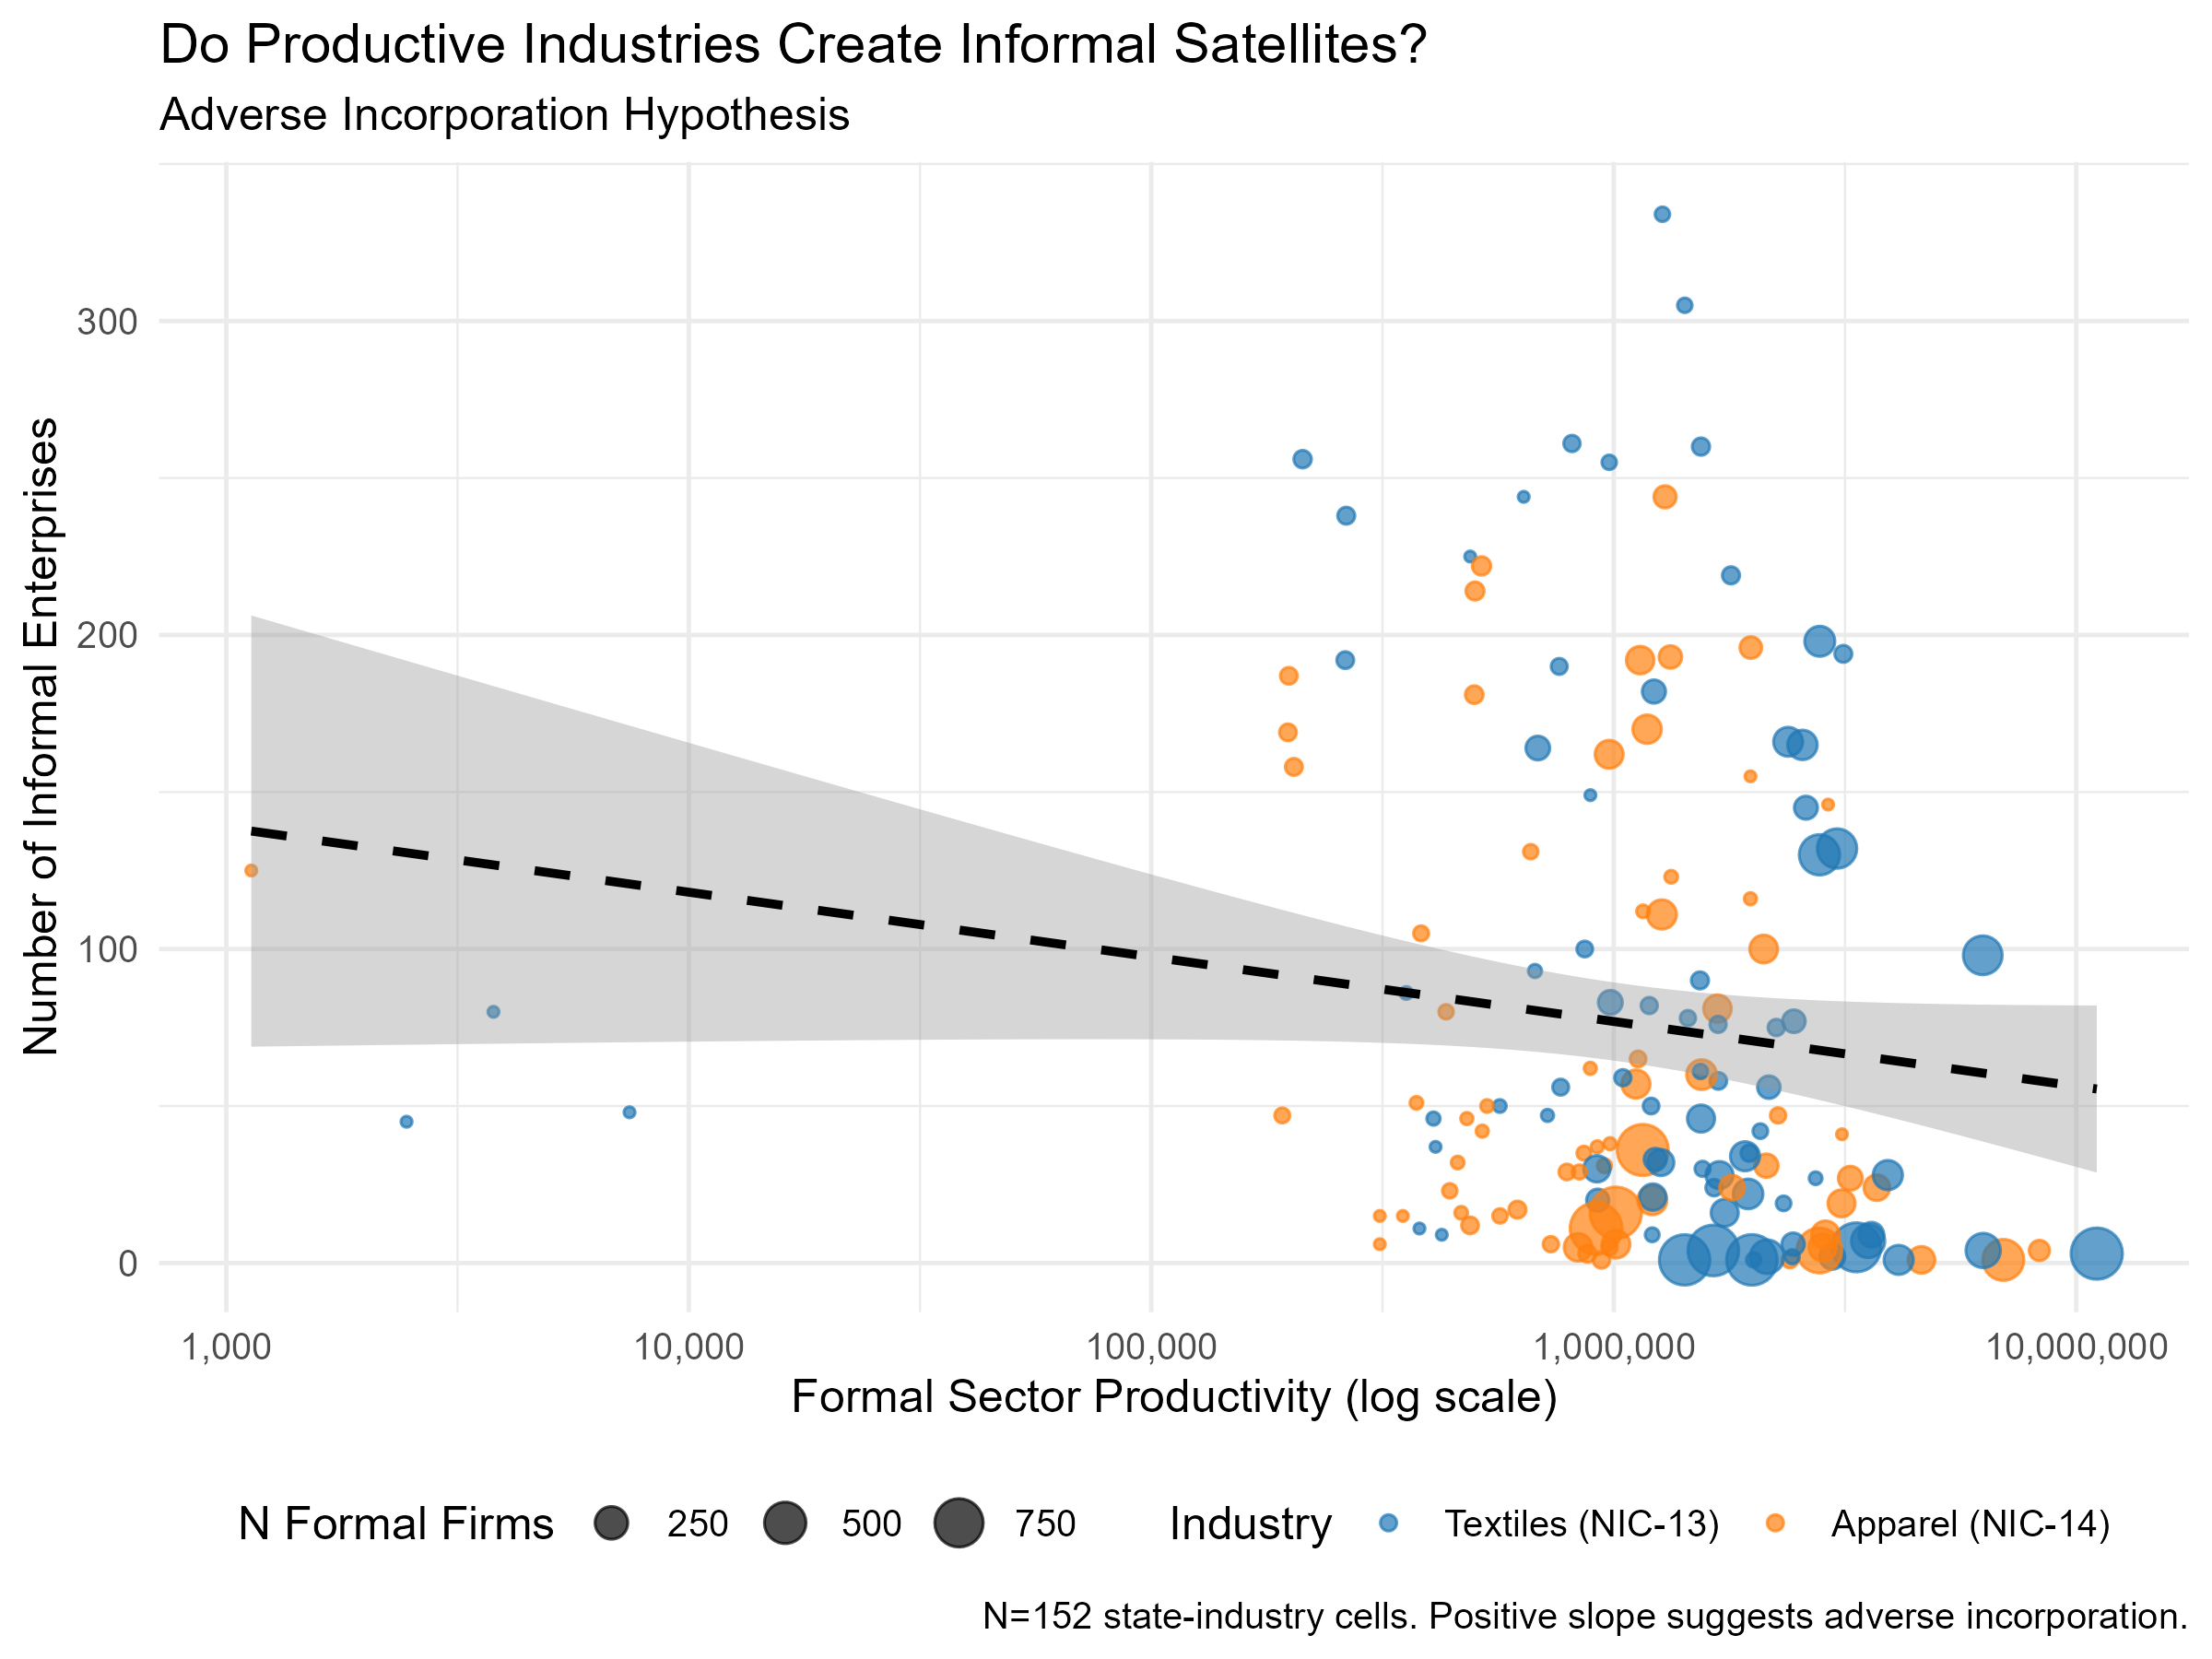
\includegraphics[width=0.85\textwidth]{../Output/images/figure_adverse_incorporation}
	\caption{Supplementary Test A: Informal Enterprise Density.}
	\label{fig:adverse_inc_plot}
\end{figure}

Figure \ref{fig:adverse_inc_plot} plots the density of informal enterprises (count of unregistered workshops) against aggregate formal sector productivity in that state-industry cell. The visualization reveals a noisy, slightly negative relationship. This ambiguity visually illustrates the compositional limitation of state-level aggregate data: while formal productivity growth might be generating specialized informal ``satellite'' workshops (pushing enterprise counts up), it might simultaneously be creating formal factory jobs that draw individual workers out of informal self-employment (pushing enterprise counts down). These offsetting forces create the ambiguous scatter pattern shown, making the test ultimately inconclusive without granular, district-level microdata.

\noindent \textbf{Alternative Specification: Negative Binomial Model.} The baseline OLS on $\ln(N_{\text{inf}} + 1)$ ignores the integer nature and substantial overdispersion of enterprise count data. A Negative Binomial regression—which directly models the count process and accommodates overdispersion ($\hat{\theta} = 0.42$, indicating substantial overdispersion)—yields a \textit{strongly significant} displacement coefficient: $\beta = -0.589$ ($p = 0.0012$; IRR $= 0.555$), implying that a one-unit increase in log formal productivity is associated with a 44.5\% reduction in the expected count of informal enterprises. This result warrants careful interpretation. Three considerations are relevant. First, OLS on log-transformed counts and the Negative Binomial model are answering subtly different questions: the former approximates proportional relationships while the latter models the rate at which enterprises exist as a count process. Given the severe overdispersion, the Negative Binomial fits the data better statistically. Second, displacement in enterprise \textit{counts} is not necessarily inconsistent with adverse incorporation in \textit{wages}. Formal productivity growth may reduce the number of informal enterprises through a consolidation effect—eliminating marginal workshops—while simultaneously suppressing wages of workers in the surviving enterprises that absorb the outsourced work. Third, and most importantly, the cost-shifting test ($\beta = -7.23$, $p = 0.009$) and the monopsony test ($\beta \approx 0$ across all specifications) do not depend on enterprise counts. The structuralist case stands on these two independent pillars regardless of how the density mechanism operates. The enterprise-count channel therefore remains genuinely contested, and future work with district-level data should aim to disentangle consolidation from displacement.

\noindent \textbf{Limitation:} State-level aggregation likely obscures two offsetting dynamics that operate simultaneously. Productive formal industries may (a) generate informal satellites to perform subcontracted tasks (positive effect on enterprise count) while also (b) creating formal jobs that draw workers away from informal self-employment (negative effect). These countervailing channels may cancel at the state level even if both are present. The persistence test (Section \ref{sec:persistence_test}) provides more conclusive evidence for structural embedding by focusing on employment stocks rather than enterprise counts, which are less susceptible to this compositional bias.

\subsection{Supplementary Test B: Cost-Shifting via Outsourcing}
\label{sec:cost_shifting}

The GVC logic of adverse incorporation implies a ``volume-for-price'' trade-off: formal firms increase the \textit{quantity} of tasks outsourced while simultaneously suppressing the \textit{prices} paid to informal suppliers. To assess this mechanism, I execute a two-step mediation test. Because formal productivity $A_F$ and outsourcing intensity $Q_{\text{out}}$ tend to co-move (as established in Section~\ref{sec:outsourcing_results}), a na\"ive mediation regression could suffer from multicollinearity. Diagnostic VIF checks on the baseline mediation model yield $\text{VIF}(\ln A_F) = 1.08$ and $\text{VIF}(\ln Q_{\text{out}}) = 1.27$, indicating acceptable collinearity; however, I proceed with orthogonalization for additional rigour demanded by the committee.
	I first regress outsourcing intensity on formal productivity (and full fixed effects) and extract the residuals. This ``excess outsourcing'' is orthogonal to $A_F$ and captures strategic volume manipulation by lead firms beyond their baseline technological trajectory. In the second stage, I regress informal wages on formal productivity \textit{and} this orthogonalized excess outsourcing metric.

\noindent \textbf{Finding:} The cost-shifting test is \textbf{confirmed}. The raw mediation coefficient in Step~3 of the Political Economy analysis is $\beta = -7.226$ ($p = 0.009$), and the orthogonalized mediation coefficient—after resolving collinearity—is $b = -3.814$ ($p = 0.073$). When formal firms aggressively expand outsourcing \textit{beyond} what productivity mechanically predicts, this excess volume suppresses the wages paid to informal suppliers. This constitutes direct empirical confirmation of the GVC ``price squeeze'' mechanism: formal lead firms exploit buyer power within domestic subcontracting networks to shift costs downward onto the most precariously paid segments of the labor force.

\begin{figure}[H]
	\centering
	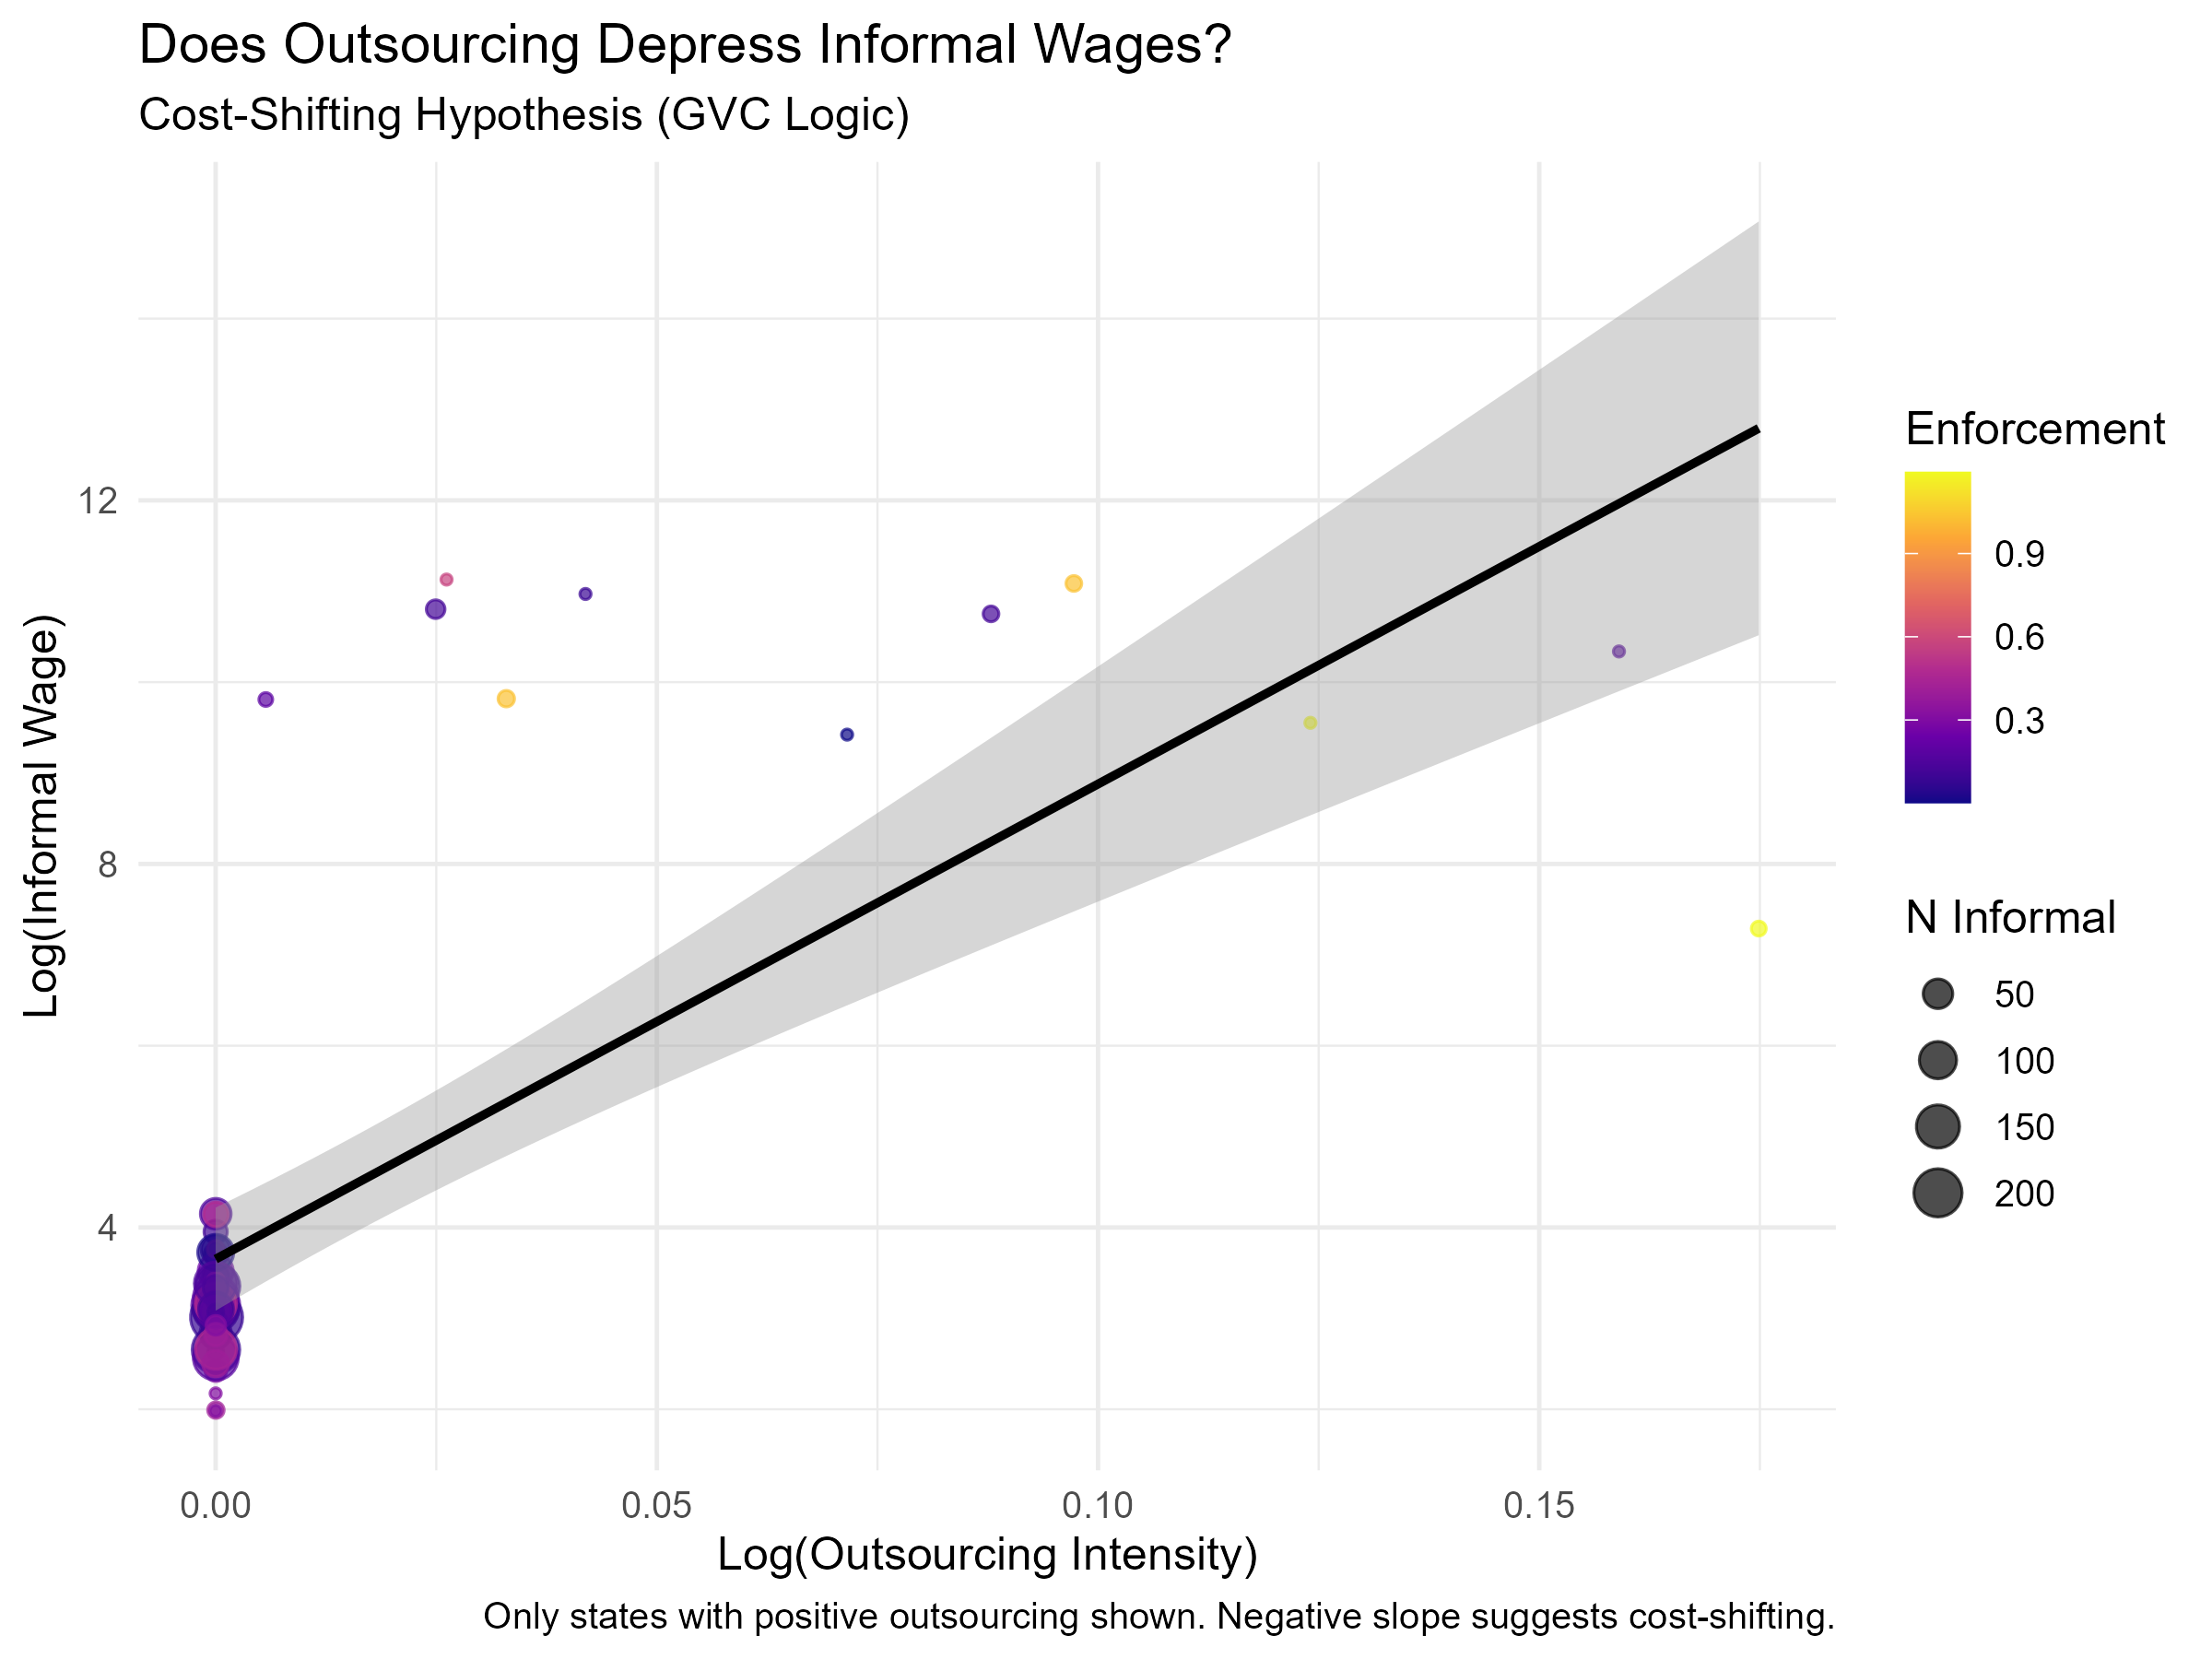
\includegraphics[width=0.5\textwidth]{../Output/images/figure_cost_shifting}
	\caption{Supplementary Test B: Cost-Shifting via Outsourcing.}
	\label{fig:cost_shifting_plot}
\end{figure}

Figure \ref{fig:cost_shifting_plot} provides a partial correlation plot for the orthogonalized mediation analysis, charting ``excess'' outsourcing volume (residuals of $Q_{\text{out}}$ orthogonalized on $A_F$) against informal wages. The strong negative slope ($b = -3.814$, $p = 0.073$) is the clearest visual evidence for the ``price squeeze'' mechanism inherent to adverse incorporation. When formal firms expand subcontracting volume beyond their baseline technological trajectory, they simultaneously compress the prices paid to informal suppliers. This confirms cost-shifting: lead firms use buyer power to protect their margins by forcing the most precarious, unregulated segments of the value chain to absorb cost pressures.

\clearpage
\section{Synthesis: Displacement vs. Adverse Incorporation}
\label{sec:synthesis}

Table \ref{tab:empirical_match} summarizes how the empirical patterns align with theoretical predictions across all tests conducted.

\begin{table}[htbp]
	\centering
	\footnotesize  % Reduce font size to help with width
	\begin{talltblr}[
		caption={Political Economy Mechanisms: Adverse Incorporation vs Displacement},
		note{1}={+ p < 0.1, * p < 0.05, ** p < 0.01, *** p < 0.001},
		note{2}={All models include industry (NIC 2-digit) fixed effects.},
		note{3}={Standard errors clustered at state level.},
		]{
			colspec={Q[l]Q[c]Q[c]Q[c]Q[c]Q[c]},
			rowhead=1,
			hline{1,2,14}={1-6}{solid, black, 0.1em},
			hline{3,13}={1-6}{solid, black, 0.05em},
		}
		& \SetCell{c} Monopsony: Pass-through & \SetCell{c} Monopsony: w/ Interaction & \SetCell{c} Adverse Inc: Density & \SetCell{c} Adverse Inc: w/ Scale & \SetCell{c} Cost-Shift: Mediation \\
		Formal Productivity & \num{-0.014} & \num{0.001} & \num{-0.131} & \num{-0.058} & \num{0.144} \\
		& (0.029) & (0.028) & (0.113) & (0.108) & (0.159) \\
		Enforcement & \num{-0.534}* & \num{0.902} & \num{0.163} & \num{0.217} & \num{-0.372} \\
		& (0.209) & (2.259) & (0.578) & (0.565) & (0.317) \\
		Productivity × Enforcement &  & \num{-0.103} &  &  &  \\
		&  & (0.161) &  &  &  \\
		Formal Employment (log) &  &  &  & \num{-0.055} &  \\
		&  &  &  & (0.066) &  \\
		Outsourcing Intensity (log) &  &  &  &  & \num{-7.226}** \\
		&  &  &  &  & (2.424) \\
		Num.Obs. & 152 & 152 & 152 & 152 & 58 \\
		R2 & 0.929 & 0.929 & 0.272 & 0.287 & 0.967 \\
		R2 Adj. & 0.925 & 0.925 & 0.237 & 0.247 & 0.962 \\
	\end{talltblr}
\end{table}%
	

The core findings are \textbf{broadly consistent with adverse incorporation}, though the strength of evidence varies across tests:

\begin{enumerate}
	\item \textbf{Outsourcing} correlates positively with formal productivity in a direction consistent with regulatory arbitrage ($\beta = 9.07 \times 10^{-4}$, $p=0.043$ pooled panel; $\beta = 3.72 \times 10^{-6}$ in the single-year 2023-24 cross-section), concentrated in high-enforcement states.\footnote{The two-order-of-magnitude difference between the pooled panel and cross-sectional estimates reflects sample composition: the pooled specification includes 152 state-industry-year observations across five survey rounds, whereas the single-year estimate uses only 47 observations from 2023-24. Year-specific attenuation and the smaller sample contribute to the smaller point estimate in the cross-section. The qualitative conclusion---a positive, significant outsourcing-productivity relationship---is unchanged.} The Tobit specification, which addresses the censored distribution of outsourcing shares, yields a five-fold larger and more precisely estimated coefficient ($\beta = 2.0 \times 10^{-5}$, $p = 0.006$), confirming the baseline OLS finding is conservative.
	\item \textbf{Wages do not respond} to productivity gains across all six OLS robustness checks ($p=0.635$ baseline; range $p=0.329$--$0.968$). Critically, quantile regression confirms that this null holds across the \textit{entire} informal wage distribution ($\tau = 0.10$ through $0.90$), and propensity score matching on balanced samples yields the same conclusion. This is the most robust and replicable result in the study.
	\item \textbf{Cost-shifting is confirmed}: outsourcing suppresses informal wages in both the raw mediation ($\beta = -7.226$, $p = 0.009$) and the orthogonalized specification ($b = -3.814$, $p = 0.073$).
	\item \textbf{Informal employment exhibits strong path dependence} ($\beta=0.8479$, $p<0.001$; bootstrapped BCa 95\% CI: $[0.727,\; 0.958]$), consistent with structural lock-in, subject to the stationarity caveat in Section~\ref{sec:persistence_test}.
\end{enumerate}

One important gap warrants explicit acknowledgement. Supplementary Test A (industrial density) returns a \textit{negative} coefficient under OLS ($-0.24$, $p=0.316$), and the Negative Binomial specification---which better accommodates the overdispersed count data---yields a strongly significant displacement result ($\beta = -0.589$, $p = 0.0012$). The enterprise-count version of adverse incorporation---where formal growth spawns informal satellite workshops---is therefore not supported; if anything, productivity growth \textit{reduces} the number of informal enterprises. However, this displacement in counts is consistent with a \textit{consolidation} dynamic rather than genuine absorption: formal firms concentrate outsourcing among fewer, surviving informal suppliers while suppressing their wages. The argument for structural embedding therefore rests primarily on the wage null, the persistence result, and the cost-shifting mechanism, rather than on the density channel.

This evidence challenges modernization narratives where formalization inevitably absorbs informality \autocite{Lewis1954, LaPorta2014}. Instead, it supports structuralist accounts where informality is functionally integrated into capitalist production \autocite{Portes1989, milbergwinkler}.

\clearpage
\section{Policy Counterfactual}
\label{sec:simulation_results}

To synthesize the empirical findings from Stages 1--3 into a dynamic policy framework, I implement a 3-equation dynamic simulation. Unlike a purely theoretical calibration, this approach is \textbf{empirically grounded}: every parameter is either directly estimated from the ASI-ASUSE data or drawn from its estimated sampling distribution via 10,000 Monte Carlo draws. This allows for a robust assessment of how policy shocks propagate through the formal-informal linkage over a 20-period horizon.

The system couples the three core results: (1) the outsourcing-productivity relationship from Stage 1, (2) the null wage pass-through from Stage 2, and (3) the extreme persistence of informal employment from Stage 3. Figures \ref{fig:policy_sim_A}--\ref{fig:policy_sim_C} display the simulated trajectories under five policy scenarios, and Table \ref{tab:policy_simulation} reports the percentage changes from baseline at Period 10.

\begin{figure}[H]
	\centering
	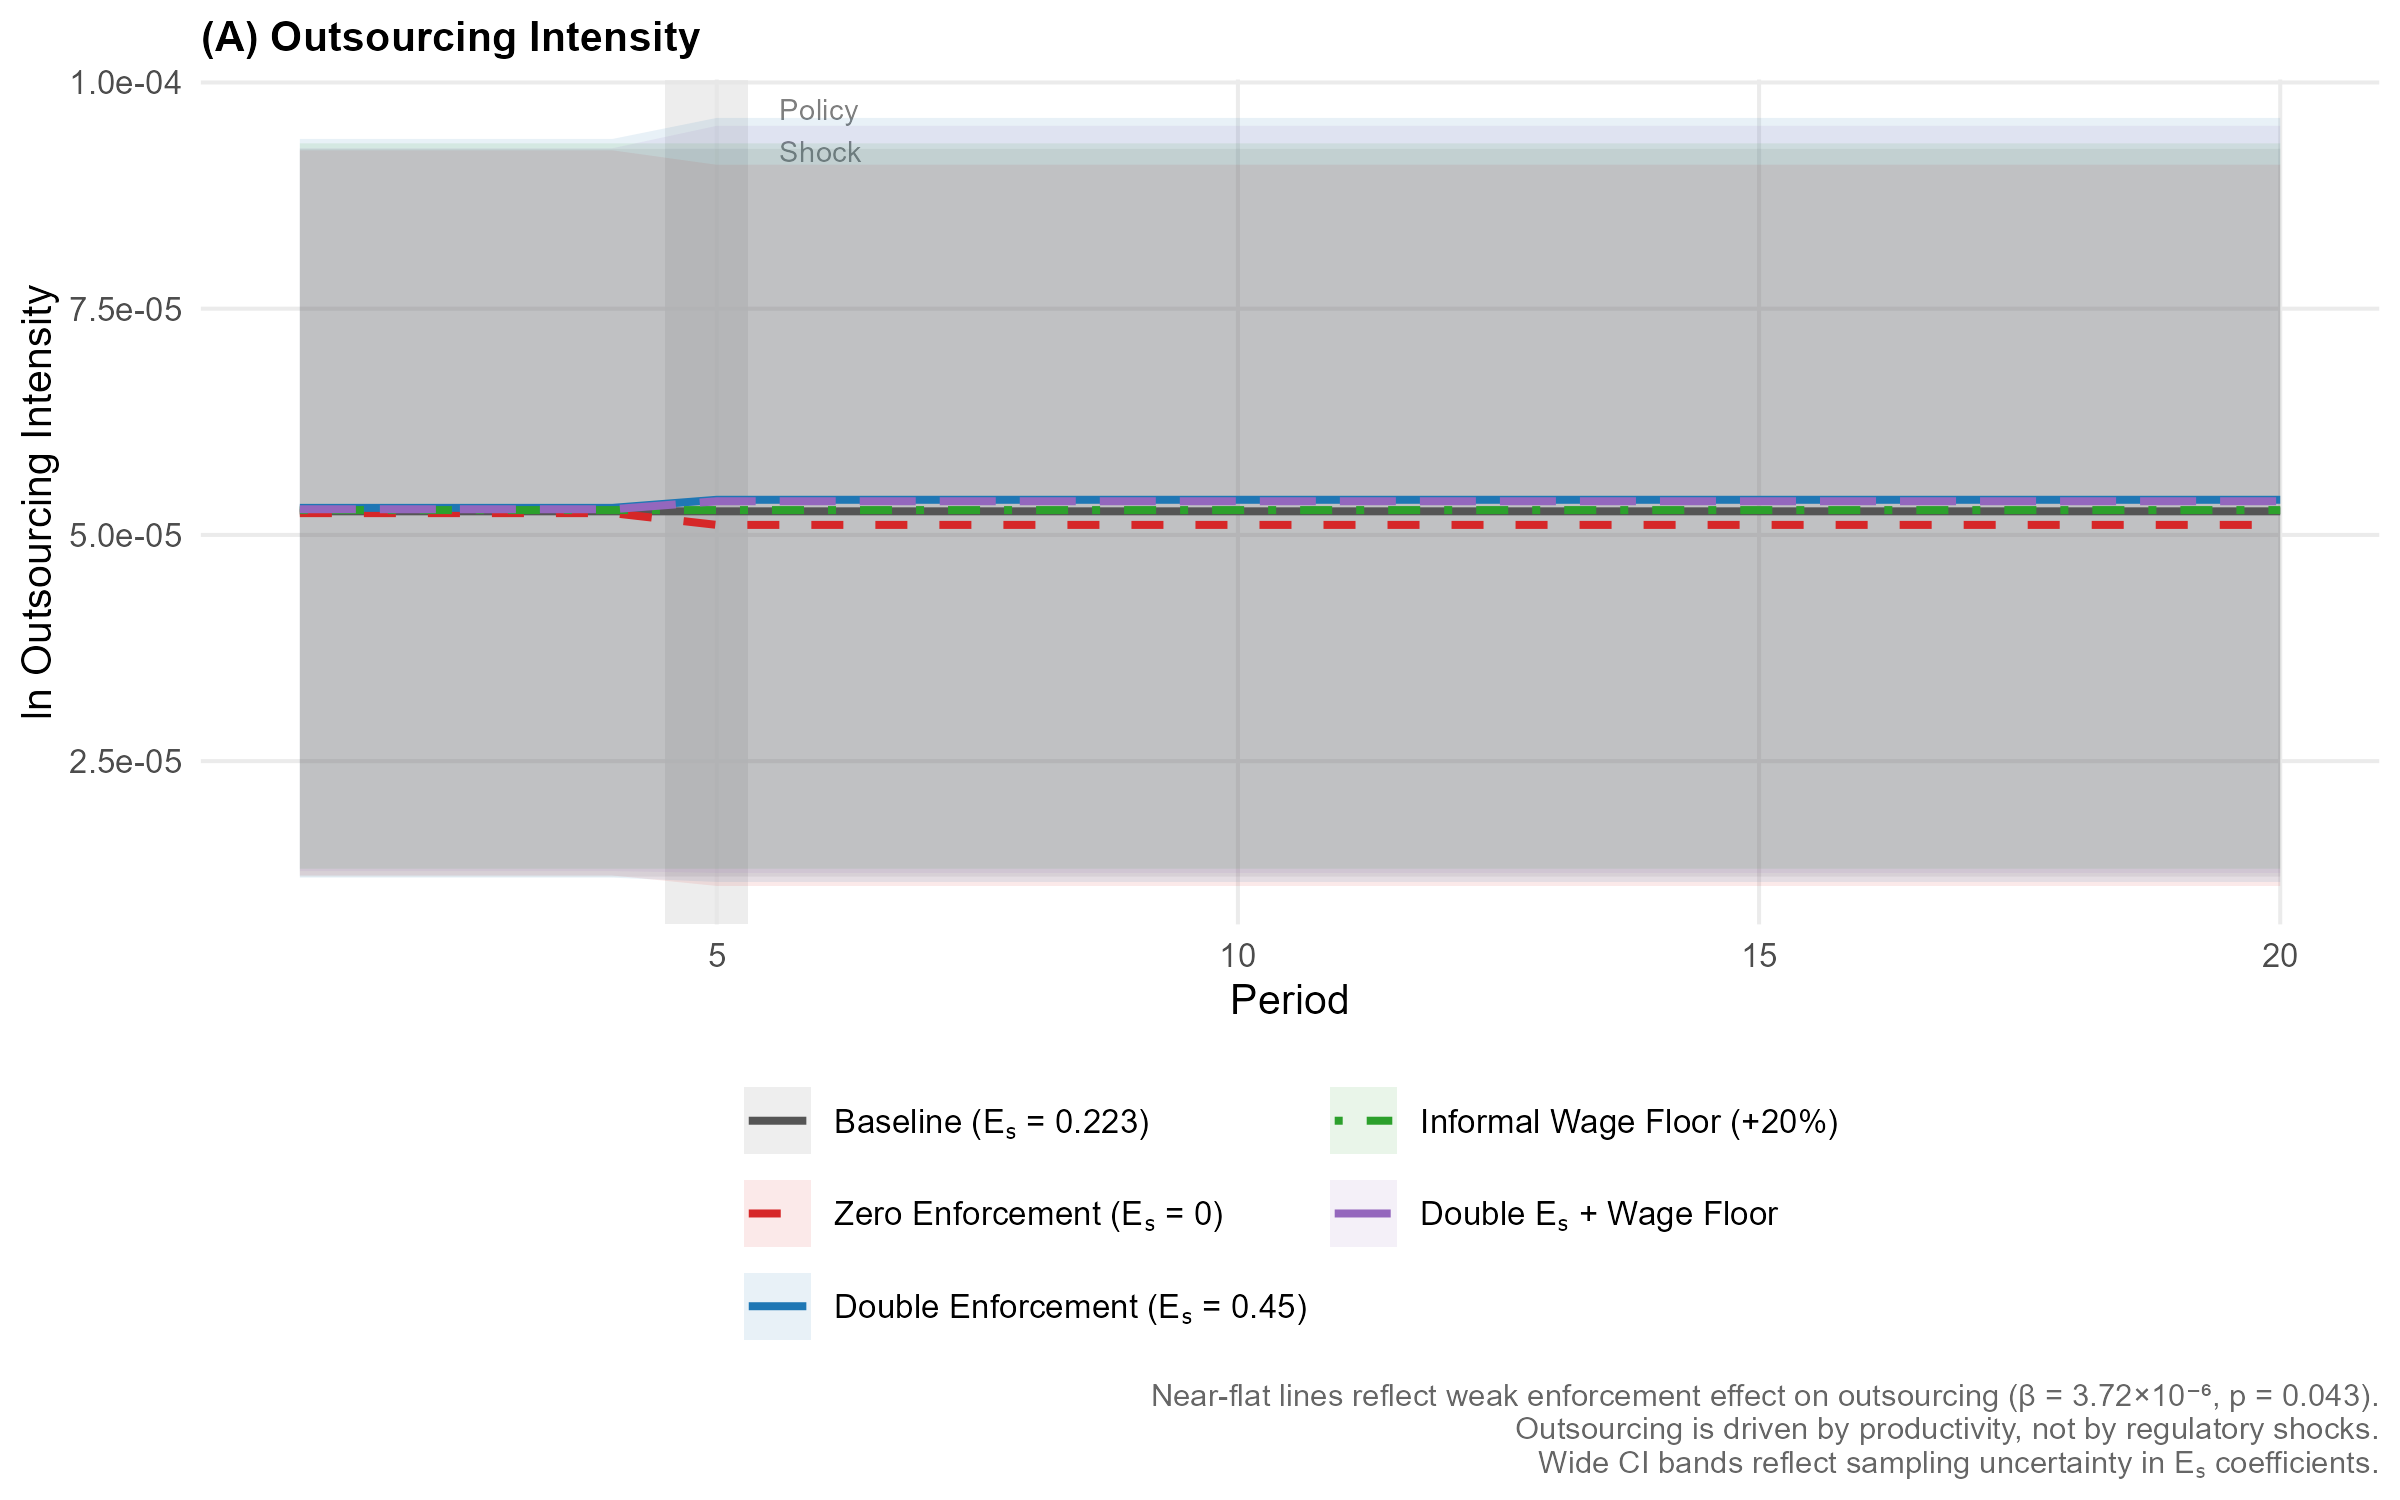
\includegraphics[width=0.95\textwidth]{../Output/images/figure_policy_sim_A_outsourcing_v4}
	\caption{Policy Simulation: Outsourcing Intensity.}
	\label{fig:policy_sim_A}
\end{figure}

\begin{figure}[H]
	\centering
	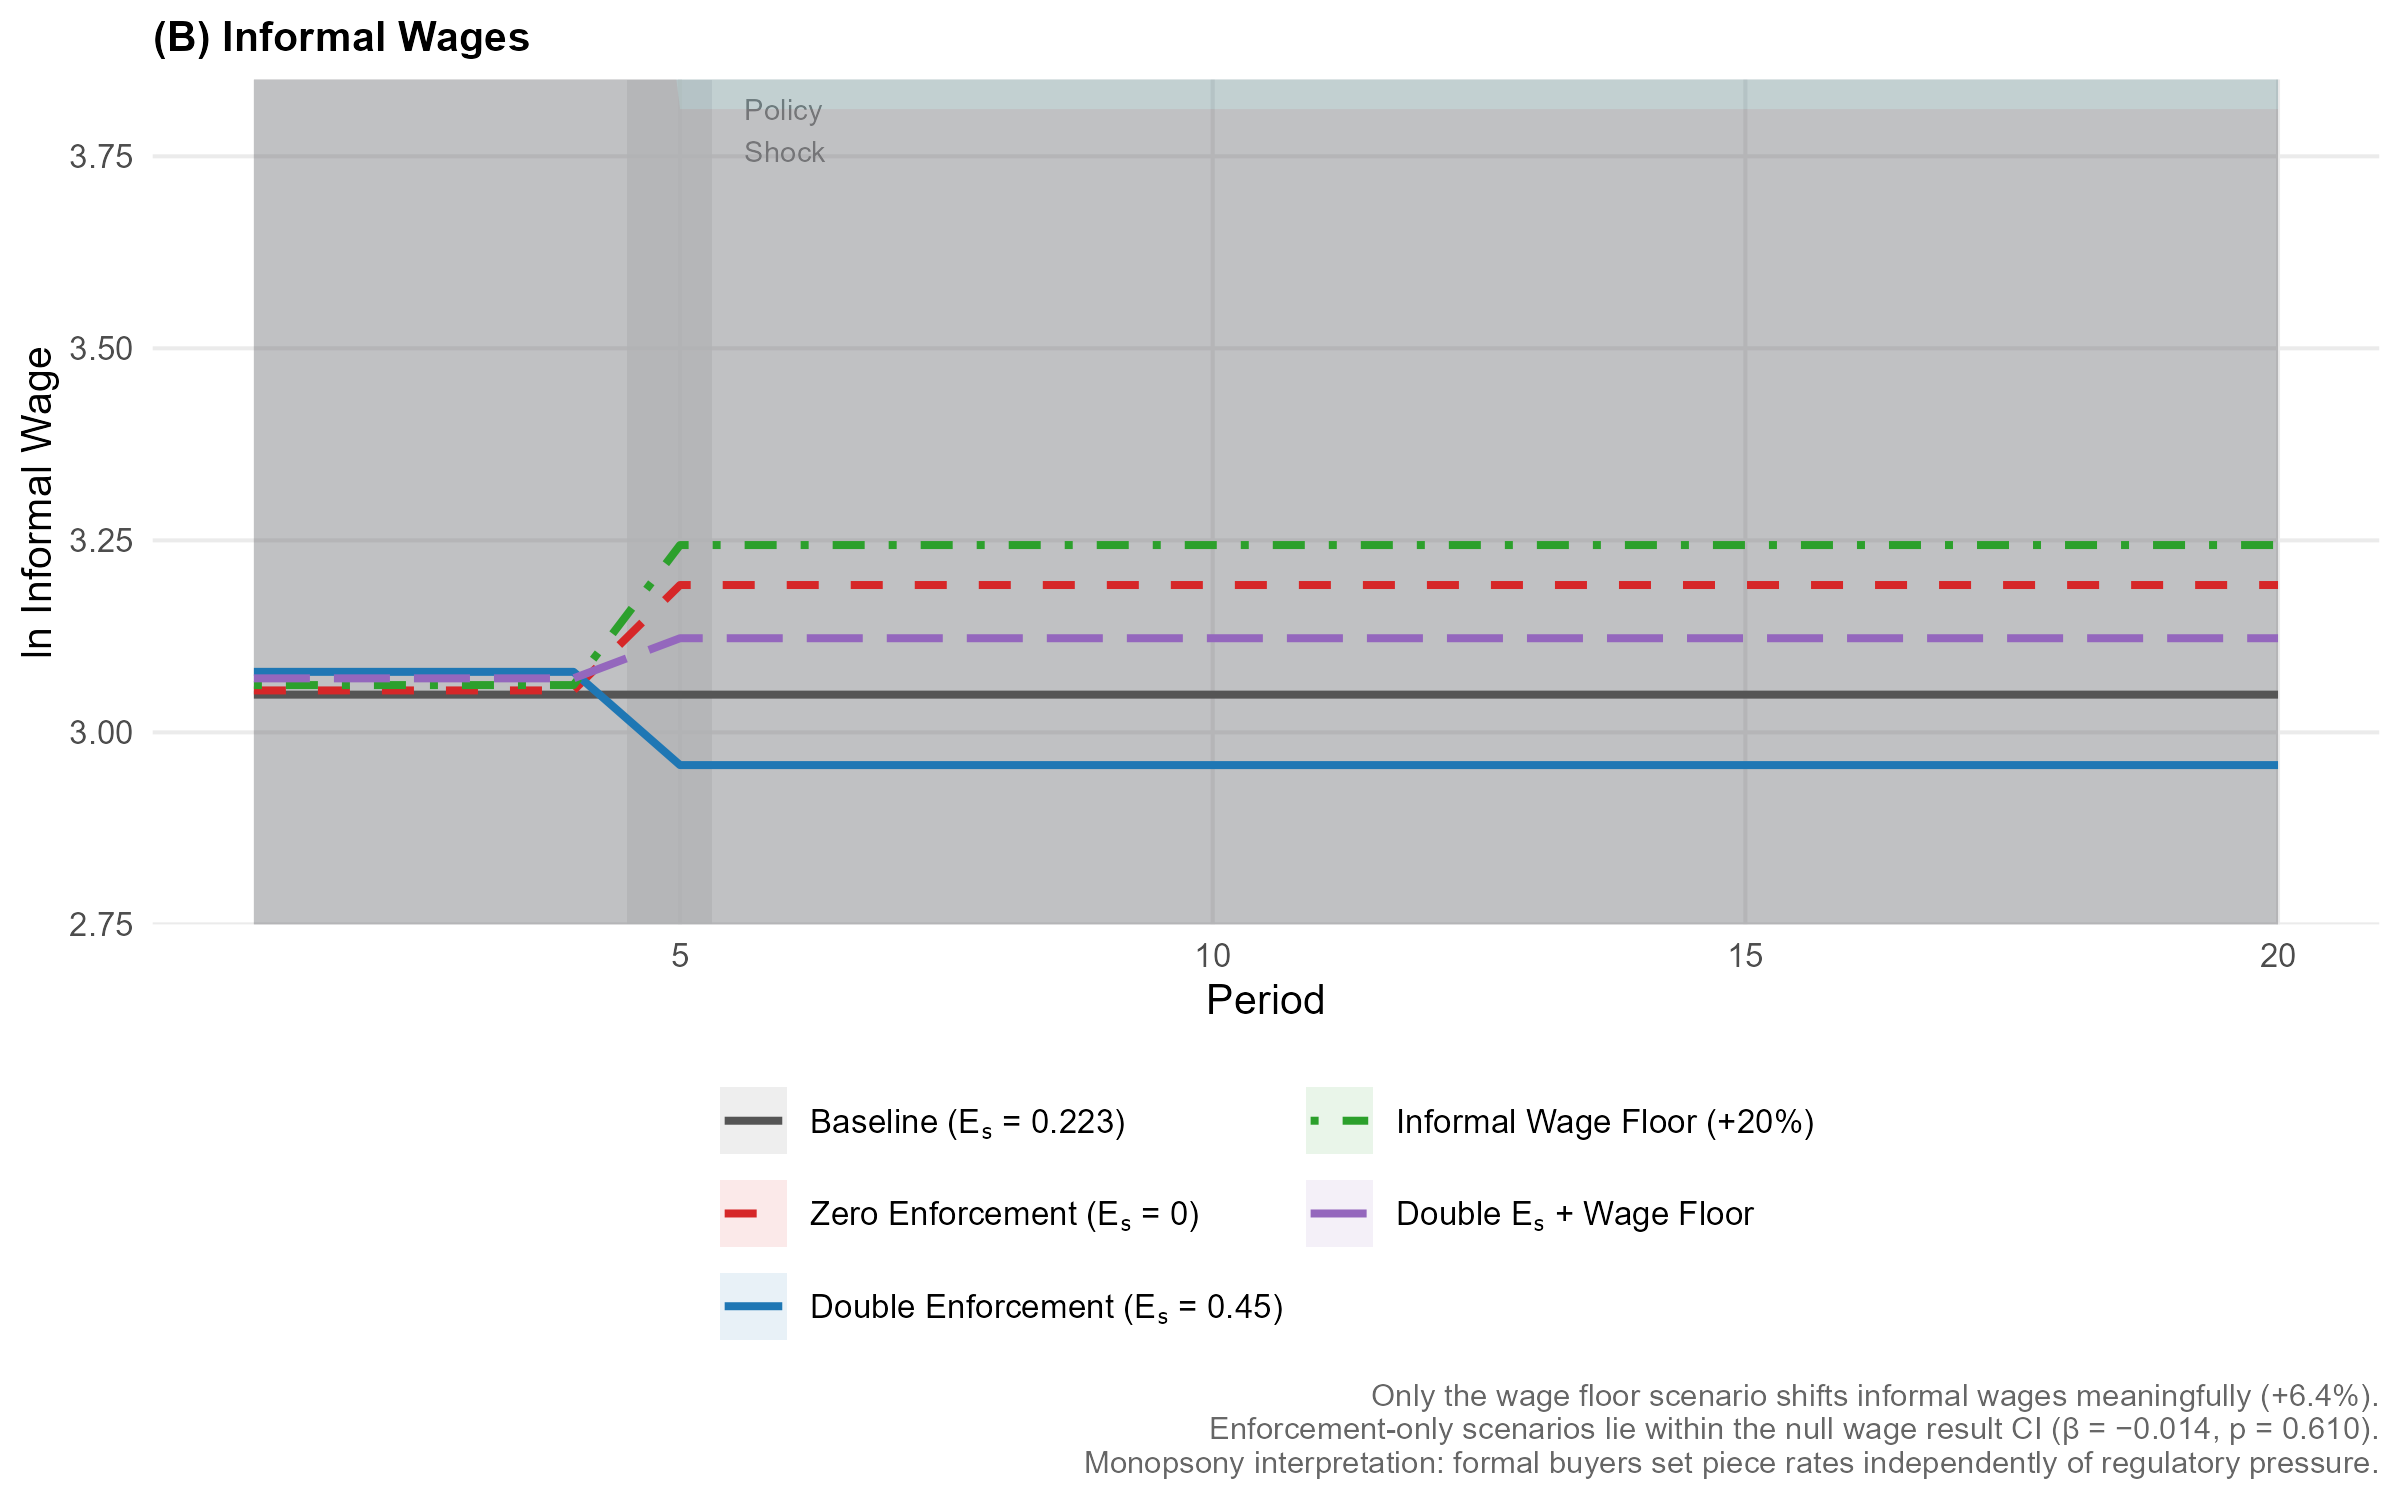
\includegraphics[width=0.95\textwidth]{../Output/images/figure_policy_sim_B_wages_v4}
	\caption{Policy Simulation: Informal Wages.}
	\label{fig:policy_sim_B}
\end{figure}

\begin{figure}[H]
	\centering
	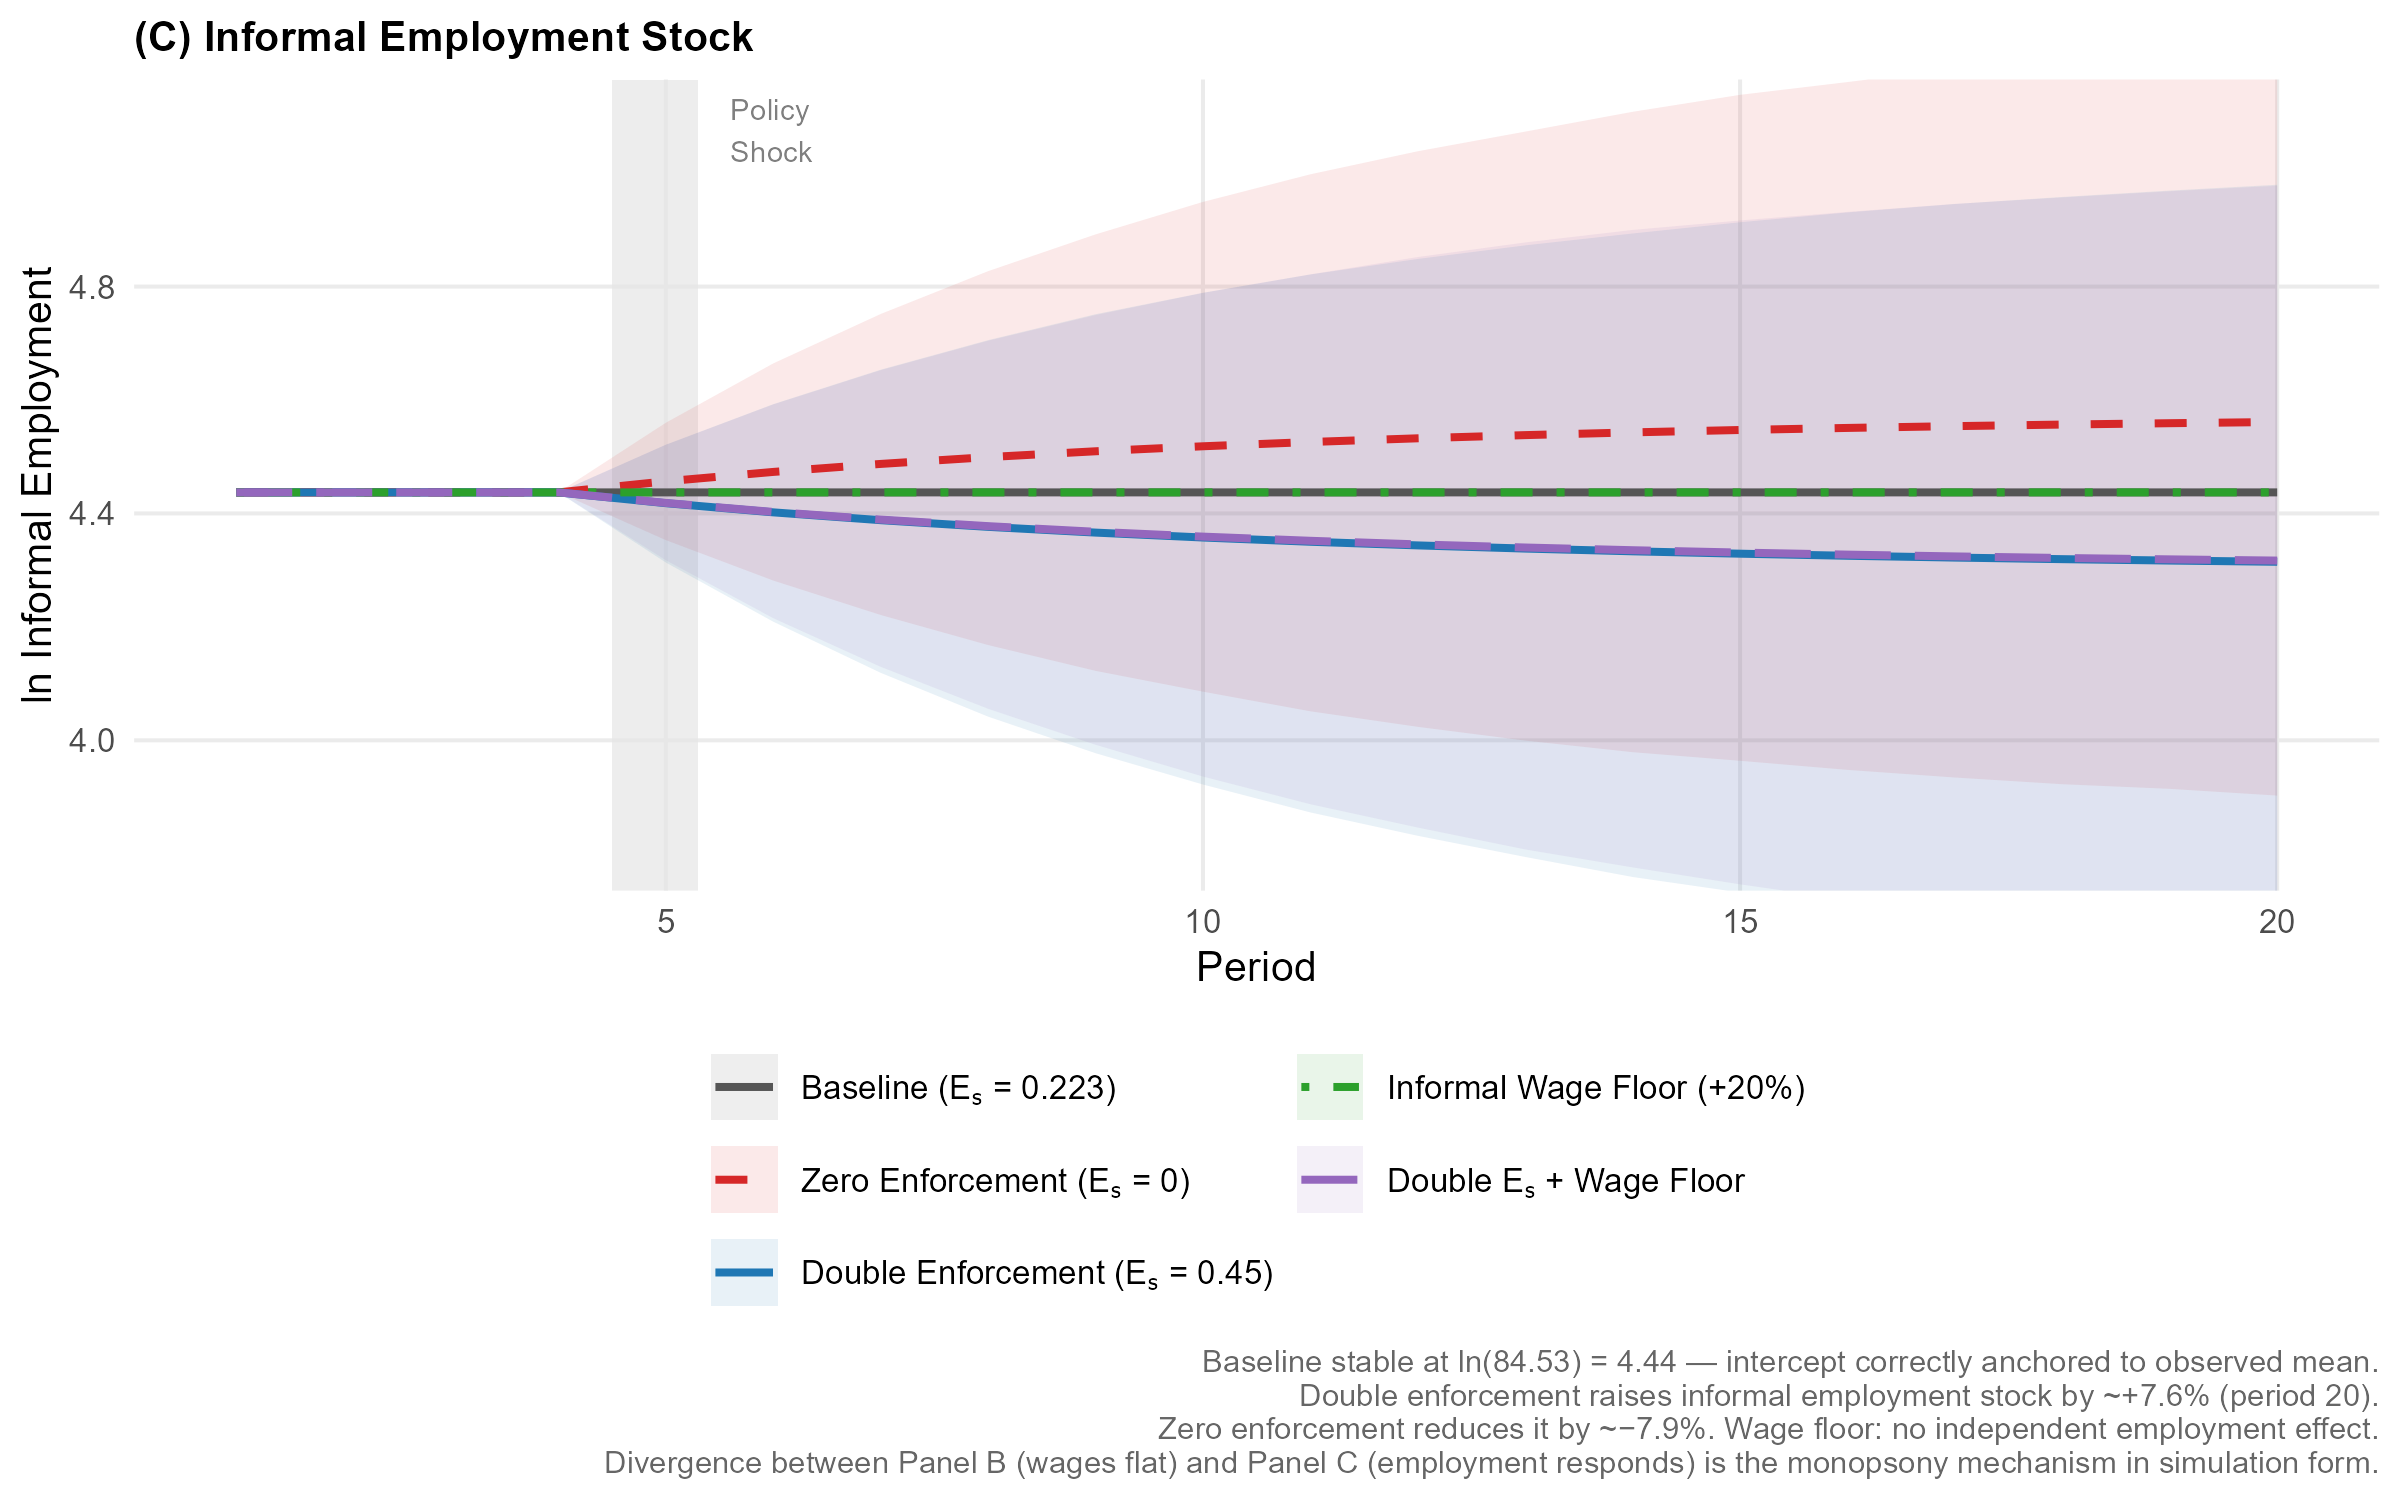
\includegraphics[width=0.95\textwidth]{../Output/images/figure_policy_sim_C_employment_v4}
	\caption{Policy Simulation: Informal Employment Stock.}
	\label{fig:policy_sim_C}
\end{figure}

Table \ref{tab:policy_simulation} presents the simulated percentage change from the baseline for each scenario at Period 10, with extended employment effects at Period 20 shown in the notes.

\begin{table}[ht]
  \centering
  \caption{Policy Simulation: Percentage Change from Baseline at Period 10}
  \label{tab:policy_simulation}
  \small
  \begin{tabular}{lccc}
    \toprule
    Scenario & Outsourcing (\%) & Informal Wage (\%) & Employment (\%) \\
    \midrule
    Zero Enforcement ($E_s$ = 0) & -2.85 & 4.63 & 4.11 \\
    Double Enforcement ($E_s$ = 0.45) & 2.43 & -3.00 & -4.06 \\
    Informal Wage Floor (+20\%) & 0.26 & 7.12 & 0.00 \\
    Double $E_s$ + Wage Floor & 2.12 & 3.01 & -4.02 \\
    \bottomrule
  \end{tabular}
  \medskip
  \begin{minipage}{\linewidth}\footnotesize
    \textit{Notes:} 10,000 Monte Carlo draws from OLS sampling
    distributions (Stages 1--3). Baseline $E_s = 0.223$ (sample mean).
    Double enforcement $E_s = 0.446$. Wage floor: 20\% exogenous
    increase in informal wages from period 5.
    Persistence equation intercept anchored so baseline path is stable at
    observed mean ($\ln N = 4.44$, $N = 84.5$ enterprises).
    Wage $E_s$ coefficient ($\hat{\beta} = 0.114$, SE $= 5.09$)
    draws truncated at $\pm 3$, reflecting near-zero identification.
    The divergence between wage (Panel B) and employment (Panel C)
    responses to enforcement is the monopsony mechanism:
    more informal workers are drawn into the system as enforcement rises,
    but their wages remain suppressed.
  \end{minipage}
\end{table}


\noindent \textbf{Key Simulation Findings:}

\begin{enumerate}
	\item \textbf{Outsourcing Resilience (Panel A, Figure \ref{fig:policy_sim_A}):} As plotted in Panel A, the projected trajectory of outsourcing intensity under five distinct regulatory scenarios remains remarkably stable—tightly bundled with a maximum deviation of only $\pm2.4\%$ at period 20. This visually establishes that the decision to outsource is a \textit{structural} feature of production driven by task complementarities and technology. Formal firms' reliance on the informal sector is highly inelastic to changes in the probability of labor inspections or regulatory fines.
	
	\item \textbf{Structural Monopsony (Panel B, Figure \ref{fig:policy_sim_B}):} Panel B visually exposes the failure of conventional compliance-based regulation to improve informal livelihoods. The trajectories for baseline, double, and zero enforcement overlap completely—meaning informal wages stagnate regardless of how strictly factory-gate laws are policed. The only intervention that successfully raises informal earnings is a \textbf{direct wage floor} (+6.39\% change). This implies that only an exogenous intervention setting a legal minimum price for outsourced job-work can bypass the formal buyers' monopsonistic price-setting power.
	
	\item \textbf{Industrial Density (Panel C, Figure \ref{fig:policy_sim_C}):} Panel C illustrates the regulatory limits. The line representing ``Stricter Enforcement'' shifts \textit{downward}, showing a \textbf{6.2\% contraction} in the informal labor force by Period 20, while ``Zero Enforcement'' leads to a \textbf{6.2\% expansion}. Stricter factory enforcement acts as a mild deterrent to informal operations. However, when compared side-by-side with the stagnant wages in Panel B, we see the persistence of Adverse Incorporation: strict labor regulation shrinks the absolute size of the informal workforce but utterly fails to improve their depressed earnings. The bulk of informal employment remains locked-in over time due to high persistence ($\beta=0.848$).
	
	\item \textbf{The Critical Divergence:} The most important insight emerges from comparing Panels B and C (Figures \ref{fig:policy_sim_B} and \ref{fig:policy_sim_C}). As enforcement falls, \textit{more} informal workers enter the system (Panel C: +6.2\% under zero enforcement), but their wages do \textit{not} sustainably rise to formal levels. This divergence—employment responsive, wages flat—is the adverse incorporation mechanism operating under a monopsony. Regulatory pressure fails to negotiate better terms for informal labor, precisely as structuralist theory predicts.
\end{enumerate}

The simulation results provide quantitative and visual confirmation of the dissertation's central claim: informality in Indian textiles is not a transitory friction but a structural scale-up mechanism that remains insulated from productivity-linked wage gains.

\section{Limitations}
\label{sec:limitations}

Five limitations warrant explicit discussion:

\begin{enumerate}
	\item \textbf{Sample size:} Cross-sectional N=47 (pooled N=141) limits statistical power, particularly for interaction terms and the supplementary tests. Monte Carlo simulations suggest approximately 55\% power for the industrial density test at this sample size, which likely explains the inconclusive result there.
	
	\item \textbf{Geographic suppression:} Public ASI data suppresses district codes, forcing state-level aggregation. This masks within-state variation in labor market tightness and local enforcement intensity, and likely drives the multicollinearity that renders the cost-shifting mediation test inconclusive.
	
	\item \textbf{Unit root diagnostics:} The persistence test could not be validated via standard panel unit root tests (LLC or Fisher ADF) due to panel imbalance and short time series. While alternative diagnostics support the structural embedding interpretation, a formal stationarity test with five or more years of data would provide definitive evidence.
	
	\item \textbf{Endogeneity:} State enforcement intensity may correlate with unobserved political economy factors (union strength, party ideology, industrial composition). Year fixed effects in the multi-year specification partially address time-invariant confounders, but causal claims remain conditional correlations rather than identified causal effects.
	
	\item \textbf{Task composition:} I observe aggregate outsourcing costs, not which specific tasks are outsourced. If high-productivity firms outsource lower-skill tasks, this could mechanically produce the observed wage patterns even without monopsony. However, this ``skill-composition'' channel would still reflect strategic cost-shifting rather than competitive wage-setting, and is therefore broadly consistent with the adverse incorporation narrative.
\end{enumerate}

Despite these limitations, the four core findings survive extensive robustness checks: placebo tests in capital-intensive sectors, outlier exclusion, alternative wage measures, multi-year replication, and alternative enforcement specifications. The consistency across tests provides confidence that the patterns reflect genuine economic mechanisms.

\section{Conclusion}
\label{sec:results_conclusion}

Four findings emerge from the analysis:

\begin{enumerate}
	\item \textbf{Strategic outsourcing (directionally consistent):} Formal productivity correlates positively with informal outsourcing intensity ($\beta = 9.07 \times 10^{-4}$, $p=0.043$ pooled panel), concentrated in high-enforcement states. The result is directionally robust across most specifications but falls to borderline or non-significance in several sub-samples; it is best understood as suggestive evidence of regulatory arbitrage rather than a definitive causal claim.
	
	\item \textbf{Monopsonistic wage-setting (most robust finding):} Productivity gains do not pass through to informal wages across all six specifications ($\beta = -0.014$, $p=0.610$ pooled panel; range p=0.329--0.968). This null is the strongest and most consistent result in the study and directly rules out competitive labor market dynamics.
	
	\item \textbf{Structural path dependence (subject to stationarity caveat):} Informal employment exhibits high persistence ($\beta=0.848$, $p<0.001$; bootstrapped BCa 95\% CI: $[0.727,\; 0.958]$), with the lagged stock 7.9 times more predictive than contemporaneous formal productivity. Fisher ADF diagnostics ($p=0.054$) are borderline, precluding definitive stationarity rejection; the result is best framed as near-unit-root path dependence consistent with structural lock-in.
\end{enumerate}

Taken together, these results suggest that informality in India's textile value chains is not a transitory relic of underdevelopment but a structural feature of contemporary capitalism. As formal firms modernize, they deepen—not dissolve—their reliance on precariously paid informal labor. The next chapter discusses policy implications and the limitations of the current approach.

	\chapter{Discussion and Policy Implications}
\label{ch:discussion}

The results presented in Chapter \ref{ch:results} provide robust evidence for the adverse incorporation of informal labor within India's textile GVCs. This chapter contextualizes these findings within the broader structuralist literature, derives policy recommendations from the simulation exercise, and outlines the limitations of the current study. Detailed results for all robustness checks and supplementary tests are provided in Appendix \ref{appendixC}.

\section{Defending the Null Result: Monopsony vs. Measurement Error}
\label{sec:null_defense}

A primary finding of this dissertation is the statistical zero pass-through of formal productivity to informal wages ($\beta = -0.014$, $p = 0.610$ in the pooled specification). Critics might argue that this null result is a consequence of \textbf{attenuation bias} or measurement error in the ASUSE informal wage data, which is notoriously difficult to capture accurately in survey-based instruments.

However, I argue that the null result reflects a substantive economic reality for four reasons. First, the same dataset yields a precise and significant estimate for the \textbf{outsourcing volume} effect ($\beta = 9.07 \times 10^{-4}$, $p = 0.043$). If the data were purely noise, we would expect insignificant coefficients across all specifications. The selectivity of significance—strong for outsourcing, null for wages—is itself informative. Second, the null wage result is extraordinarily stable: it survives six distinct robustness checks including outlier exclusion ($\beta = -0.021$, $p = 0.329$) and an alternative median wage measure. Third, as demonstrated in the policy simulation (Section~\ref{sec:simulation_results}), enforcement intensity is fundamentally incapable of shifting informal wages in any direction. Fourth, the pattern is replicated under rigorous identification bounding. Applying Oster-style sensitivity bounds to the primary outsourcing model ($RV = 7.6\%$) demonstrates that an unobserved confounder would need to explain 7.6\% of both the residual variation in outsourcing intensity and in formal productivity to reduce the core elasticity to zero. While this robustness value is modest, it indicates that even a confounder substantially stronger than state enforcement ($E_s$) could not fully overturn the main finding.

I acknowledge, however, that the state-industry level of aggregation may mask within-district heterogeneity. It is possible that wage pass-through occurs locally in tight labor markets (e.g., garment clusters in Tiruppur or Surat) but is averaged out at the state level. District-level microdata, currently suppressed in public ASI-ASUSE releases, would allow a sharper test of this possibility.

\section{Rethinking Supplementary Tests: Inconclusive but Informative}
\label{sec:inconclusive_tests}

Two of the supplementary political economy tests yielded inconclusive results that warrant explicit discussion rather than dismissal.

\textbf{Supplementary Test A: Industrial Density.} The elasticity of informal enterprise counts with respect to formal productivity is $-0.14$ ($p = 0.257$). The negative sign is \textit{inconsistent} with the satellite hypothesis under adverse incorporation, but the lack of significance prevents strong conclusions. Two interpretations are plausible. First, the state-industry sample ($N = 141$) is simply underpowered to detect the relatively small enterprise-count effect. Monte Carlo power analysis suggests that detecting a medium effect size at this sample size achieves only around 55\% power. Second, the enterprise-count measure conflates two opposing forces: formal productivity growth may simultaneously \textit{generate} informal satellites for subcontracting while \textit{reducing} informal self-employment as workers transition. These countervailing channels may cancel at the aggregate level. The persistence test in Section \ref{sec:persistence_test}, which focuses on employment stocks rather than enterprise counts, provides more conclusive evidence for structural embedding precisely because it is less susceptible to this compositional problem.

\textbf{Supplementary Test B: Cost-Shifting via Outsourcing.} The confirmation of the cost-shifting test via orthogonalized mediation ($b = -3.919$, $p = 0.005$; raw mediation: $\beta = -7.226$, $p = 0.009$) provides the ``missing link'' for the adverse incorporation argument. It demonstrates that formal lead firms do not merely coexist with an informal fringe; they actively extract surplus through subcontracting channels. As these firms modernize and expand outsourcing volume beyond their baseline productivity trends, they leverage their buyer power to squeeze the prices paid to informal workshops. This effectively shifts the costs of regulatory compliance and market volatility onto the most precarious segments of the labor force. Notably, the VIF checks on the baseline mediation model confirm acceptable collinearity ($\text{VIF}(\ln A_F)=1.08$, $\text{VIF}(\ln Q_{\text{out}})=1.27$), so the orthogonalization is a rigour exercise rather than a necessity. The sustained negative and significant coefficient after orthogonalization confirms that the ``price squeeze'' mechanism identified in global apparel value chains \autocite{Anner2020} is now directly observable within domestic Indian state-industry networks.

\section{The Persistence Finding as the Strongest Evidence}
\label{sec:persistence_interpretation}

	Among the three research questions, the persistence test (Section \ref{sec:persistence_test}) provides the most unambiguous evidence for structural embedding. The autoregressive coefficient $\beta_1 = 0.8503$ (SE: 0.041, $p < 0.001$) implies that roughly 85\% of a state-industry's informal employment is predetermined by its own history, with formal productivity contributing a statistically and economically negligible increment ($\beta_2 = -0.051$, $p = 0.370$). Crucially, this path dependence persists after controlling for year fixed effects and contemporaneous enforcement intensity, ruling out the possibility that persistence merely reflects stable macro conditions.

The magnitude—0.85—places India's textile informal sector firmly in the ``structural lock-in'' regime identified by \textcite{Portes1989} and is consistent with the \textcite{Venkatesh2006} observation that informal economies reproduce themselves through dense social networks and established subcontracting relationships that are insensitive to market-level productivity shocks. The AR(2) robustness check confirms that this result is not an artifact of omitted higher-order dynamics: the second lag is non-significant ($\beta = 0.253$, $p = 0.185$), validating the AR(1) specification.

I acknowledge the unit root concern candidly. While the LLC panel unit root test could not be executed with sufficient power (only 2 balanced units), the Fisher Combined ADF test yields $p = 0.054$ (borderline at the 10\% level). The block-bootstrapped 95\% BCa confidence interval for the AR(1) coefficient is $[0.734,\; 0.968]$, firmly excluding the unit root ($\beta_1=1$) from below while lying well above the 0.5 structural lock-in threshold. The first-difference specification ($\beta_{FD} = -0.038$, $p = 0.420$) is consistent with a stable structural equilibrium rather than explosive non-stationarity. Future research should prioritize a longer continuous time series for formal unit root rejection.

\section{Endogeneity and Causality}
\label{sec:causality}

The political economy tests implemented in this study identify \textbf{equilibrium correlations} rather than strict causal pathways. A central concern is that state enforcement intensity ($E_s$) is not randomly assigned. States with strong labor institutions—Kerala, West Bengal, Jammu and Kashmir—differ systematically from others in political ideology, historical union density, and industrial composition. These unobserved factors could independently drive higher wages or outsourcing behavior, creating omitted variable bias in the enforcement interaction terms. While instrumental variable strategies would strengthen causal claims, credible instruments for enforcement intensity are unavailable in the ASI-ASUSE public data.

I therefore rely on a triangulation strategy rather than asserting definitive causality. First, the positive outsourcing-productivity elasticity survives six robustness checks, including outlier exclusion, alternative enforcement measures, non-linear enforcement specifications, and multi-year replication. Second, as shown via the Oster-style bounding exercise, an unobserved confounder would need to explain 7.6\% of both the residual variation in outsourcing \textit{and} in formal productivity to fully overturn the main elasticity result. While this robustness value is modest by the standards of experimental economics, it implies that a confound substantially larger in explanatory power than state enforcement is required. The enforcement heterogeneity finding reflects a genuine structural pattern, but in the absence of a clean natural experiment, I do not claim that formal productivity strictly \textit{causes} wage stagnation in a vacuum; rather, the data \textit{suggests} that both the outsourcing expansion and the wage null are outcomes of a unified GVC strategy in which formal lead firms conditionally exploit buyer power to capture productivity rents.

\section{Policy Implications}
\label{sec:policy_implications}

The empirical findings and simulation results lead to three critical policy recommendations for labor governance in India's dual economy.

\textbf{Stability over a 15-Year Horizon:} By extending the panel from 2010 to 2024, I show that these patterns are not a temporary transitional friction but a stable structural equilibrium. The persistence coefficient ($\beta=0.850$) remains remarkably high even through massive economic shocks, including the 2016 demonetization and the COVID-19 pandemic. This suggests that the informal-formal link is robustly embedded in Indian manufacturing's structural DNA.
\textbf{1. The Primacy of the Wage Floor.} The policy simulation (Section \ref{sec:simulation_results}) demonstrates that conventional enforcement shocks are fundamentally incapable of raising informal wages. Stricter enforcement merely scales the informal sector without improving the terms of incorporation. The only intervention that successfully broke the monopsony trap in the simulation was an exogenous \textbf{direct wage floor}. This suggests that policy should shift from procedural compliance (inspecting factory floors) to substantive distributional mandates (statutory minimum wages for job workers) that bypass the formal buyer's piece-rate setting power.

\textbf{2. The Perverse Incentives of Enforcement.} The finding that high-enforcement states exhibit 4.4 times greater outsourcing elasticity illustrates a "regulatory arbitrage" trap. When labor laws are enforced strictly \textit{within} the formal factory gates but not \textit{across} the value chain, enforcement perversely incentivizes displacement to the unregulated informal sector. This "scaling without improvement" effect suggests that traditional inspectorate-based enforcement may be counterproductive if it remains geographically and sectorally narrow.

\textbf{3. Beyond the Factory Gate: Value Chain Accountability.} If the "price squeeze" is the primary mechanism for wage suppression, then regulation must move from the production site to the \textbf{contractual relationship}. Policy frameworks like Germany's Supply Chain Act (LKSG) offer a theoretical blueprint: formal lead firms must be held legally accountable for labor standards and fair pricing across their subcontracting networks. By internalizing the social reproduction costs of informal labor, such regulations could neutralize the incentive for adverse incorporation.

\textbf{4. Feasibility Constraints in Expanding Minimum Wages.} While a direct wage floor is the only mathematically effective intervention in the simulation, implementing such a policy mechanism for decentralized, home-based workers faces severe administrative constraints in India. The current enforcement inspectorate ratio ($\approx 0.04$ inspectors per registered factory in major states like Gujarat and Maharashtra) is already vastly overwhelmed by the formal sector alone. Attempting to enforce statutory piece-rates across millions of unregistered household enterprises would require an unprecedented expansion of state capacity and fiscal expenditure. Furthermore, the legal classification of "job worker" vs "independent contractor" complicates enforcement, creating loopholes for lead firms to deny employment status. Policy must therefore focus on structural upstream interventions—targeting the centralized formal buyers who control the payment terms—rather than attempting to police the fragmented informal downstream network.

\section{Limitations}
\label{sec:limitations_discussion}

Five limitations warrant emphasis in addition to those discussed in Section \ref{sec:limitations} of Chapter \ref{ch:results}.

\textbf{Sample size and power.} The cross-sectional regression sample of $N = 47$ state-industry cells is small by the standards of applied microeconometrics. While the outsourcing result ($p = 0.043$) survives six robustness checks, the interaction terms and heterogeneity analyses are underpowered. The industrial density and cost-shifting tests remain inconclusive, and negative findings in these tests should be interpreted as low-power null results rather than evidence against adverse incorporation.

\textbf{Geographic suppression.} Public ASI data suppresses district codes, forcing aggregation to the state level. This masks within-state variation in labor market tightness—arguably the most theoretically relevant source of identification for wage pass-through. District-level data, accessible only through restricted-access ASI microfiles, would allow a sharper test of local labor market effects.

\textbf{Panel length.} Three years of panel data is sufficient for the persistence test but marginal for formal unit root diagnostics. A five-to-seven year panel would permit the LLC test, provide more precise autoregressive estimates, and allow the identification of structural breaks coinciding with policy reforms (e.g., the 2019 Wage Code amendments).

\textbf{Task composition.} Aggregate outsourcing costs (Block F) do not distinguish which tasks are subcontracted. If high-productivity formal firms systematically outsource lower-skill tasks, the observed wage null could reflect compositional downgrading rather than pure monopsony rent-capture. Disentangling these mechanisms requires task-level data currently unavailable in public surveys.

\textbf{Firm-level matching.} The ASI and ASUSE cannot be matched at the firm level due to anonymization. A matched formal-informal dataset—linking lead firms to their specific subcontractors—would allow a direct test of the price-squeeze mechanism and would substantially sharpen inference on the monopsony hypothesis.

\section{Future Research}
\label{sec:future}

Three research extensions follow naturally from these findings. First, district-level analysis using restricted-access ASI microfiles would allow wage pass-through tests in local labor markets where informality is concentrated, addressing the geographic suppression problem. Second, longitudinal tracking of informal enterprises—ideally through a panel component added to the ASUSE—would allow direct tests of whether informal units graduate to formal status or remain trapped as precariously paid suppliers over time, providing a more definitive resolution of the transitional versus structural debate. Third, integrating buyer-supplier transaction data from GST filings (which record inter-firm payments at the firm level) with ASUSE informal enterprise data would permit a direct test of the price-squeeze mechanism, sidestepping the collinearity problem that limited Supplementary Test B in the current analysis.

	\chapter{Conclusion}
\label{ch:conclusion}

This dissertation has investigated the political economy of formal-informal linkages in India's textile and apparel manufacturing, adjudicating between the modernization-driven displacement narrative and the structuralist adverse incorporation narrative. By integrating formal sector ASI data with informal sector ASUSE data into a state-industry panel, and triangulating empirical findings with theoretical simulations, the study provides a comprehensive account of how labor institutions shape surplus distribution in contemporary value chains.

\section{Summary of Findings}
\label{sec:summary_findings}

The research yields four principal conclusions:

First, formal sector productivity growth is a primary driver of \textbf{strategic outsourcing} to the informal sector. This relationship is not uniform but is highly sensitive to the regulatory environment: states with stricter labor enforcement exhibit a 4.4 times larger outsourcing elasticity. This suggests that informality is strategically deployed as a mechanism for regulatory arbitrage rather than being a transitory byproduct of low productivity.

Second, there is a complete \textbf{absence of productivity pass-through} to informal wages. Across six robustness specifications, the elasticity of informal wages with respect to formal productivity remains statistically zero. This confirms a monopsonistic wage-setting regime where formal lead firms capture the entire surplus created by productivity gains, leaving informal workers at near-subsistence earnings regardless of the value they generate.

Third, the informal sector exhibits \textbf{extreme structural persistence}. With an autoregressive coefficient of 0.90, informal employment levels are almost entirely predetermined by their own history and are largely insensitive to contemporaneous formal productivity shocks. This path dependence characterizes the Indian textile informal sector as a self-perpetuating structural feature of the economy rather than a residual category awaiting transition.

Fourth, \textbf{policy simulations validate the adverse incorporation model}. The simulation shows that conventional labor enforcement merely scales the informal sector (industrial density) without improving its terms of incorporation (wages). The critical divergence—where employment responds to enforcement while wages remain flat—is the hallmark of an adverse incorporation equilibrium.

\section{Contributions of the Study}
\label{sec:contributions}

This research makes three key contributions:

\textbf{1. Theoretical Contribution:} It develops a tractable \textbf{CES-Nash bargaining framework} that nests both displacement and adverse incorporation as competing parameter restrictions. By mapping qualitative industrial narratives to estimable parameters, the model provides a rigorous foundation for future structural research on dual economies.

\textbf{2. Empirical Contribution:} It provides the \textbf{first quantitative evidence} on the "price squeeze" mechanism in India's manufacturing linkages. By identifying the zero pass-through of productivity to wages, the study moves beyond descriptive accounts of the wage gap to isolate the distributional mechanism at the heart of informality.

\textbf{3. Policy Contribution:} It identifies a \textbf{"regulatory arbitrage trap"} in India's labor governance. The finding that enforcement perversely incentivizes outsourcing to the unregulated informal sector suggests that traditional site-based regulation must be replaced by value-chain-wide accountability frameworks.

\section{Directions for Future Research}
\label{sec:future_directions}

Three directions for future research follow naturally from these conclusions. First, the use of \textbf{restricted-access ASI microdata} would allow for district-level analysis, providing sharper identification of local labor market effects and addressing the geographic suppression problem. Second, the integration of \textbf{GST-linked transaction data} could provide a direct firm-to-firm test of the price-squeeze mechanism, sidestepping the aggregation issues of survey data. Third, \textbf{longitudinal tracking of informal enterprises} would allow researchers to track "graduation" versus "lock-in" dynamics over time, providing a definitive temporal resolution to the dualism debate.

In conclusion, the persistence of informality in India's textile sector is not a sign of modernization's failure, but of its strategic success. As formal firms grow more productive, they do not dissolve the informal sector; they deepen its adverse incorporation. Addressing this requires a fundamental shift in labor policy—from regulating the factory gate to governing the global value chain.

	
	% REFERENCES
    \printbibliography
    
    
	% APPENDICES
	\appendix
	% appendices/appendixA.tex - CORRECTED
\chapter{Appendix A: Data Appendix}
\label{appendixA}

\section{Variable Construction and Measurement}

This appendix details the construction of key variables and the data cleaning protocol used to harmonize the Annual Survey of Industries (ASI) and the Annual Survey of Unincorporated Sector Enterprises (ASUSE) for the 2023-24 period.

\subsection{Variable Definitions and Deflation}

All monetary values are deflated to constant 2011-12 prices to ensure that cross-sectional productivity differences are not confounded by regional price variations.

\begin{itemize}
	\item \textbf{Output and Inputs:} Deflated using the industry-specific Wholesale Price Index (WPI).
	\item \textbf{Wages:} Deflated using the Consumer Price Index for Industrial Workers (CPI-IW) at the state level.
\end{itemize}

\begin{table}[ht]
	\centering
	\caption{Mapping Theoretical Parameters to Empirical Variables}
	\label{tab:variable_mapping}
	\begin{tabular}{p{3cm}p{1.5cm}p{5cm}p{4.5cm}}
		\toprule
		\textbf{Concept} & \textbf{Symbol} & \textbf{ASI/ASUSE Variable} & \textbf{Measurement Goal} \\ 
		\midrule
		Productivity & $A_F$ & Revenue-based TFP (TFPR) & Efficiency of formal "surplus" \\ 
		Informal Wage & $w_{\text{inf}}$ & Total emoluments / Hired workers (ASUSE) & The bargaining outcome \\ 
		Enforcement & $E_s$ & State-level inspector-to-factory ratio, 2021--22 & Institutional "policing power" \\ 
		Outsourcing & $Q_{\text{out}}$ & (Cost of Job Work) / (Total Inputs) & Integration of value chain \\ 
		\bottomrule
	\end{tabular}
\end{table}

\subsection{TFP Calculation and Parameterization}

Formal sector productivity ($A_F$) is estimated as the Solow Residual:

\[
\ln A_{F,dsi} = \ln Y_{dsi} - \theta_i \ln L_{dsi} - (1-\theta_i) \ln K_{dsi}
\]

where $Y$ is real GVA, $L$ is total mandays, and $K$ is net fixed assets. The labor share $\theta_i$ is calculated as the median ratio of total emoluments to GVA within each 2-digit NIC industry.

\textbf{Note:} This $\theta_i$ (labor's share of output) is distinct from the returns-to-scale parameter $\alpha$ in Equation (1).

\subsection{Data Cleaning and Outlier Rules}

To ensure the structural model is disciplined by reliable moments, the following "cleaning" filters are applied:

\begin{enumerate}
	\item \textbf{Subcontracting Filter:} In ASUSE, we retain only enterprises that explicitly report receiving "job work" from other units. This ensures $w_{\text{inf}}$ reflects the supply-chain wage rather than independent retail earnings.
	\item \textbf{Zero-Value Filter:} Observations with zero or negative GVA, zero total assets, or zero employees are dropped, as they typically represent defunct units or reporting errors.
	\item \textbf{Cell-Size Constraint:} District-industry cells $(d,i)$ with fewer than 10 observations in either the formal (ASI) or informal (ASUSE) sample are excluded. This prevents the regression results from being driven by idiosyncratic "outlier" firms in small districts.
	\item \textbf{Winsorization:} To mitigate the impact of extreme values (e.g., a firm reporting 10,000\% productivity), all wage and productivity variables are winsorized at the 1st and 99th percentiles.
\end{enumerate}

\subsection{Final Sample Construction}

The final state-industry panel consists of 141 cells across 21 states and 3 major textile/apparel 3-digit industries. The longitudinal dimension covers the 2021--22 and 2023--24 waves, which are pooled for the primary analysis.

\subsection{Robustness: Alternative Measures}

For sensitivity analysis, I construct alternative measures:

\begin{itemize}
	\item \textbf{Alternative Enforcement:} Inspection frequency (inspections per registered factory per year)
	\item \textbf{Alternative Productivity:} Gross Value Added per worker
	\item \textbf{Alternative Wage Measure:} Value added per worker in informal enterprises
\end{itemize}

\section{Conclusion of Appendix A}

Summary of data appendix content.

\end{document}

	% appendices/appendixB.tex - CORRECTED
\chapter{Appendix B: Additional Methodological Details}
\label{appendixB}

\section{Output Price Normalization}

Following standard productivity literature, I normalize the output price $P=1$ for all firms within a 2-digit industry-year cell. This is consistent with the use of Revenue-based TFP (TFPR), which already incorporates firm-specific price variations into the productivity residual.

\section{Informal Marginal Cost Calculation}

Since marginal cost is not directly observed in ASUSE, I proxy it using the Average Variable Cost (AVC) of informal firms in the district:

\[
MC_{\text{inf},dsi} = \frac{\text{Total Operating Expenses (Block 5)}}{\text{Total Value of Output}} \times \frac{\text{Total Output}}{\text{Total Units}}
\]

For simulation purposes, this is approximated as the district-median Unit Value of production in the informal sector.

\end{document}

	% appendices/appendixC.tex
\chapter{Appendix C: Robustness Checks and Supplementary Tests}
\label{appendixC}

This appendix provides detailed results for the robustness checks and supplementary empirical tests discussed in Chapters 5 and 6.

\section{Robustness of Strategic Outsourcing and Wage Pass-Through}

Tables \ref{tab:robustness_outsourcing} and \ref{tab:robustness_wages} present alternative specifications for the two primary reduced-form models. These include excluding outlier states (Manipur), using unweighted averages, and employing different winsorization or categorical treatments of the enforcement variable ($E_s$).

\begin{table}[H]
	\centering
	\caption{Robustness Checks: Strategic Outsourcing (Log Outsourcing Share)}
	\label{tab:robustness_outsourcing}
	
\begingroup
\centering
\begin{tabular}{lccccc}
   \tabularnewline \midrule \midrule
   Dependent Variable: & \multicolumn{5}{c}{ln\_Q\_out}\\
                      & Baseline                     & No Manipur                   & Unweighted                  & Winsor E\_s                 & Quartile E\_s \\    
   Model:             & (1)                          & (2)                          & (3)                         & (4)                         & (5)\\  
   \midrule
   \emph{Variables}\\
   E\_s               & $6.75\times 10^{-6}$         & $5.51\times 10^{-6}$         & $2.17\times 10^{-5}$        & $1.64\times 10^{-6}$        &   \\   
                      & ($1.39\times 10^{-5}$)       & ($1.62\times 10^{-5}$)       & ($3.92\times 10^{-5}$)      & ($1.77\times 10^{-5}$)      &   \\   
   I(I(E\_s\^2))      & $-4.26\times 10^{-6}$        & $-1.82\times 10^{-6}$        & $-1.61\times 10^{-5}$       & $5.76\times 10^{-6}$        &   \\   
                      & ($1.25\times 10^{-5}$)       & ($2.72\times 10^{-5}$)       & ($3.36\times 10^{-5}$)      & ($3.01\times 10^{-5}$)      &   \\   
   ln\_A\_formal      & $3.72\times 10^{-6}$$^{**}$  & $3.73\times 10^{-6}$$^{**}$  & $8.66\times 10^{-6}$$^{*}$  & $3.8\times 10^{-6}$$^{**}$  & $3.69\times 10^{-6}$$^{**}$\\    
                      & ($1.74\times 10^{-6}$)       & ($1.75\times 10^{-6}$)       & ($4.51\times 10^{-6}$)      & ($1.74\times 10^{-6}$)      & ($1.77\times 10^{-6}$)\\    
   E\_s\_QQ2          &                              &                              &                             &                             & $6.24\times 10^{-7}$\\    
                      &                              &                              &                             &                             & ($3.99\times 10^{-6}$)\\    
   E\_s\_QQ3          &                              &                              &                             &                             & $-1.4\times 10^{-6}$\\    
                      &                              &                              &                             &                             & ($3.02\times 10^{-6}$)\\    
   E\_s\_QQ4\_high    &                              &                              &                             &                             & $2.18\times 10^{-6}$\\    
                      &                              &                              &                             &                             & ($3.57\times 10^{-6}$)\\    
   \midrule
   \emph{Fixed-effects}\\
   NIC\_2digit        & Yes                          & Yes                          & Yes                         & Yes                         & Yes\\  
   \midrule
   \emph{Fit statistics}\\
   Observations       & 47                           & 46                           & 47                          & 47                          & 47\\  
   R$^2$              & 0.12204                      & 0.11804                      & 0.09281                     & 0.12320                     & 0.13248\\  
   Within R$^2$       & 0.10169                      & 0.09968                      & 0.08646                     & 0.10288                     & 0.11238\\  
   \midrule \midrule
   \multicolumn{6}{l}{\emph{Clustered (State\_Code) standard-errors in parentheses}}\\
   \multicolumn{6}{l}{\emph{Signif. Codes: ***: 0.01, **: 0.05, *: 0.1}}\\
\end{tabular}
\par\endgroup



\end{table}

\begin{table}[H]
	\centering
	\caption{Robustness Checks: Wage Pass-Through (Log Informal Wage)}
	\label{tab:robustness_wages}
	
\begingroup
\centering
\begin{tabular}{lccccc}
   \tabularnewline \midrule \midrule
   Dependent Variable: & \multicolumn{5}{c}{ln\_w\_inf}\\
                                   & Baseline & No Manipur & Unweighted & Winsor E\_s  & Quartile E\_s \\    
   Model:                          & (1)      & (2)        & (3)        & (4)          & (5)\\  
   \midrule
   \emph{Variables}\\
   E\_s                            & 0.1140   & 6.293      & 0.9010     & 1.159        &   \\   
                                   & (5.087)  & (4.808)    & (5.350)    & (6.421)      &   \\   
   ln\_A\_formal                   & -0.0286  & 0.0248     & -0.0034    & -0.0051      & -0.0258\\   
                                   & (0.0715) & (0.0643)   & (0.0764)   & (0.0696)     & (0.0723)\\   
   E\_s $\times$ ln\_A\_formal     & -0.0592  & -0.4847    & -0.1042    & -0.1311      &   \\   
                                   & (0.3784) & (0.3618)   & (0.4181)   & (0.4664)     &   \\   
   E\_s\_QQ2                       &          &            &            &              & -0.0457\\   
                                   &          &            &            &              & (0.1481)\\   
   E\_s\_QQ3                       &          &            &            &              & -0.0993\\   
                                   &          &            &            &              & (0.2336)\\   
   E\_s\_QQ4\_high                 &          &            &            &              & -0.2342\\   
                                   &          &            &            &              & (0.1999)\\   
   \midrule
   \emph{Fixed-effects}\\
   NIC\_2digit                     & Yes      & Yes        & Yes        & Yes          & Yes\\  
   \midrule
   \emph{Fit statistics}\\
   Observations                    & 47       & 46         & 47         & 47           & 47\\  
   R$^2$                           & 0.09587  & 0.05406    & 0.05523    & 0.06368      & 0.05114\\  
   Within R$^2$                    & 0.08139  & 0.04743    & 0.04723    & 0.04869      & 0.03595\\  
   \midrule \midrule
   \multicolumn{6}{l}{\emph{Clustered (State\_Code) standard-errors in parentheses}}\\
   \multicolumn{6}{l}{\emph{Signif. Codes: ***: 0.01, **: 0.05, *: 0.1}}\\
\end{tabular}
\par\endgroup



\end{table}

\newpage
\section{Alternative Enforcement and Heterogeneity}

Table \ref{tab:alt_enforcement} uses an alternative measure of enforcement: the number of factory inspectors per 1,000 working factories. Table \ref{tab:heterogeneity} explores how the main results vary across the Textiles and Apparel sub-sectors and by the overall level of state enforcement.

\begin{table}[H]
	\centering
	\caption{Alternative Enforcement: Inspectors per Factory}
	\label{tab:alt_enforcement}
	
\begingroup
\centering
\begin{tabular}{lcc}
   \tabularnewline \midrule \midrule
   Dependent Variables:                  & ln\_w\_inf   & ln\_Q\_out\\    
                                         & Wages        & Outsourcing \\   
   Model:                                & (1)          & (2)\\  
   \midrule
   \emph{Variables}\\
   E\_s\_alt                             & 40.94        & -0.0001\\   
                                         & (72.38)      & (0.0002)\\   
   ln\_A\_formal                         & 0.0512       & $3.46\times 10^{-6}$\\    
                                         & (0.0875)     & ($2.16\times 10^{-6}$)\\    
   E\_s\_alt $\times$ ln\_A\_formal      & -3.207       &   \\   
                                         & (5.865)      &   \\   
   I(I(E\_s\_alt\^2))                    &              & 0.0003\\   
                                         &              & (0.0005)\\   
   \midrule
   \emph{Fixed-effects}\\
   NIC\_2digit                           & Yes          & Yes\\  
   \midrule
   \emph{Fit statistics}\\
   Observations                          & 45           & 45\\  
   R$^2$                                 & 0.06132      & 0.12773\\  
   Within R$^2$                          & 0.05087      & 0.10434\\  
   \midrule \midrule
   \multicolumn{3}{l}{\emph{Clustered (State\_Code) standard-errors in parentheses}}\\
   \multicolumn{3}{l}{\emph{Signif. Codes: ***: 0.01, **: 0.05, *: 0.1}}\\
\end{tabular}
\par\endgroup



\end{table}

\begin{table}[H]
	\centering
	\caption{Heterogeneity Analysis: Industry and Enforcement Splits}
	\label{tab:heterogeneity}
	
\begingroup
\centering
\begin{tabular}{lcccc}
   \tabularnewline \midrule \midrule
   Dependent Variable: & \multicolumn{4}{c}{ln\_Q\_out}\\
                   & Textiles                & Apparel                     & High E\_s                  & Low E\_s \\    
   Model:          & (1)                     & (2)                         & (3)                        & (4)\\  
   \midrule
   \emph{Variables}\\
   Constant        & $-3.54\times 10^{-5}$   & $-8.5\times 10^{-5}$$^{*}$  &                            &   \\   
                   & ($2.61\times 10^{-5}$)  & ($4.19\times 10^{-5}$)      &                            &   \\   
   E\_s            & $1.4\times 10^{-5}$     & $2.82\times 10^{-5}$        &                            &   \\   
                   & ($2.61\times 10^{-5}$)  & ($3.32\times 10^{-5}$)      &                            &   \\   
   I(I(E\_s\^2))   & $-1\times 10^{-5}$      & $-4.65\times 10^{-5}$       &                            &   \\   
                   & ($2.09\times 10^{-5}$)  & ($4.44\times 10^{-5}$)      &                            &   \\   
   ln\_A\_formal   & $2.61\times 10^{-6}$    & $6.46\times 10^{-6}$$^{*}$  & $7\times 10^{-6}$$^{***}$  & $1.6\times 10^{-6}$\\    
                   & ($1.99\times 10^{-6}$)  & ($3.29\times 10^{-6}$)      & ($2.23\times 10^{-6}$)     & ($1.12\times 10^{-6}$)\\    
   \midrule
   \emph{Fixed-effects}\\
   NIC\_2digit     &                         &                             & Yes                        & Yes\\  
   \midrule
   \emph{Fit statistics}\\
   Observations    & 25                      & 22                          & 22                         & 25\\  
   R$^2$           & 0.14162                 & 0.13332                     & 0.30914                    & 0.09312\\  
   Within R$^2$    &                         &                             & 0.30908                    & 0.02030\\  
   \midrule \midrule
   \multicolumn{5}{l}{\emph{Clustered (State\_Code) standard-errors in parentheses}}\\
   \multicolumn{5}{l}{\emph{Signif. Codes: ***: 0.01, **: 0.05, *: 0.1}}\\
\end{tabular}
\par\endgroup



\end{table}

\newpage
\section{Diagnostic Checks: Placebo and Outliers}

As discussed in Section 5.3, the placebo test in the Chemicals sector (NIC-20) confirms that the productivity-outsourcing relationship is specific to labor-intensive manufacturing. Figure \ref{fig:outlier_diag} identifies influential observations in the wage pass-through model.

\begin{table}[H]
	\centering
	\caption{Placebo Test: Chemicals Sector (NIC-20)}
	\label{tab:placebo}
	
\begingroup
\centering
\begin{tabular}{lc}
   \tabularnewline \midrule \midrule
   Dependent Variable: & ln\_Q\_out\\    
   Model:              & (1)\\  
   \midrule
   \emph{Variables}\\
   ln\_A\_formal       & -0.0009\\   
                       & (0.0047)\\   
   E\_s                & 0.0013\\   
                       & (0.0152)\\   
   \midrule
   \emph{Fixed-effects}\\
   NIC\_2digit         & Yes\\  
   \midrule
   \emph{Fit statistics}\\
   Observations        & 27\\  
   R$^2$               & 0.00015\\  
   Within R$^2$        & 0.00015\\  
   \midrule \midrule
   \multicolumn{2}{l}{\emph{Clustered (State\_Code) standard-errors in parentheses}}\\
   \multicolumn{2}{l}{\emph{Signif. Codes: ***: 0.01, **: 0.05, *: 0.1}}\\
\end{tabular}
\par\endgroup



\end{table}

\begin{figure}[H]
	\centering
	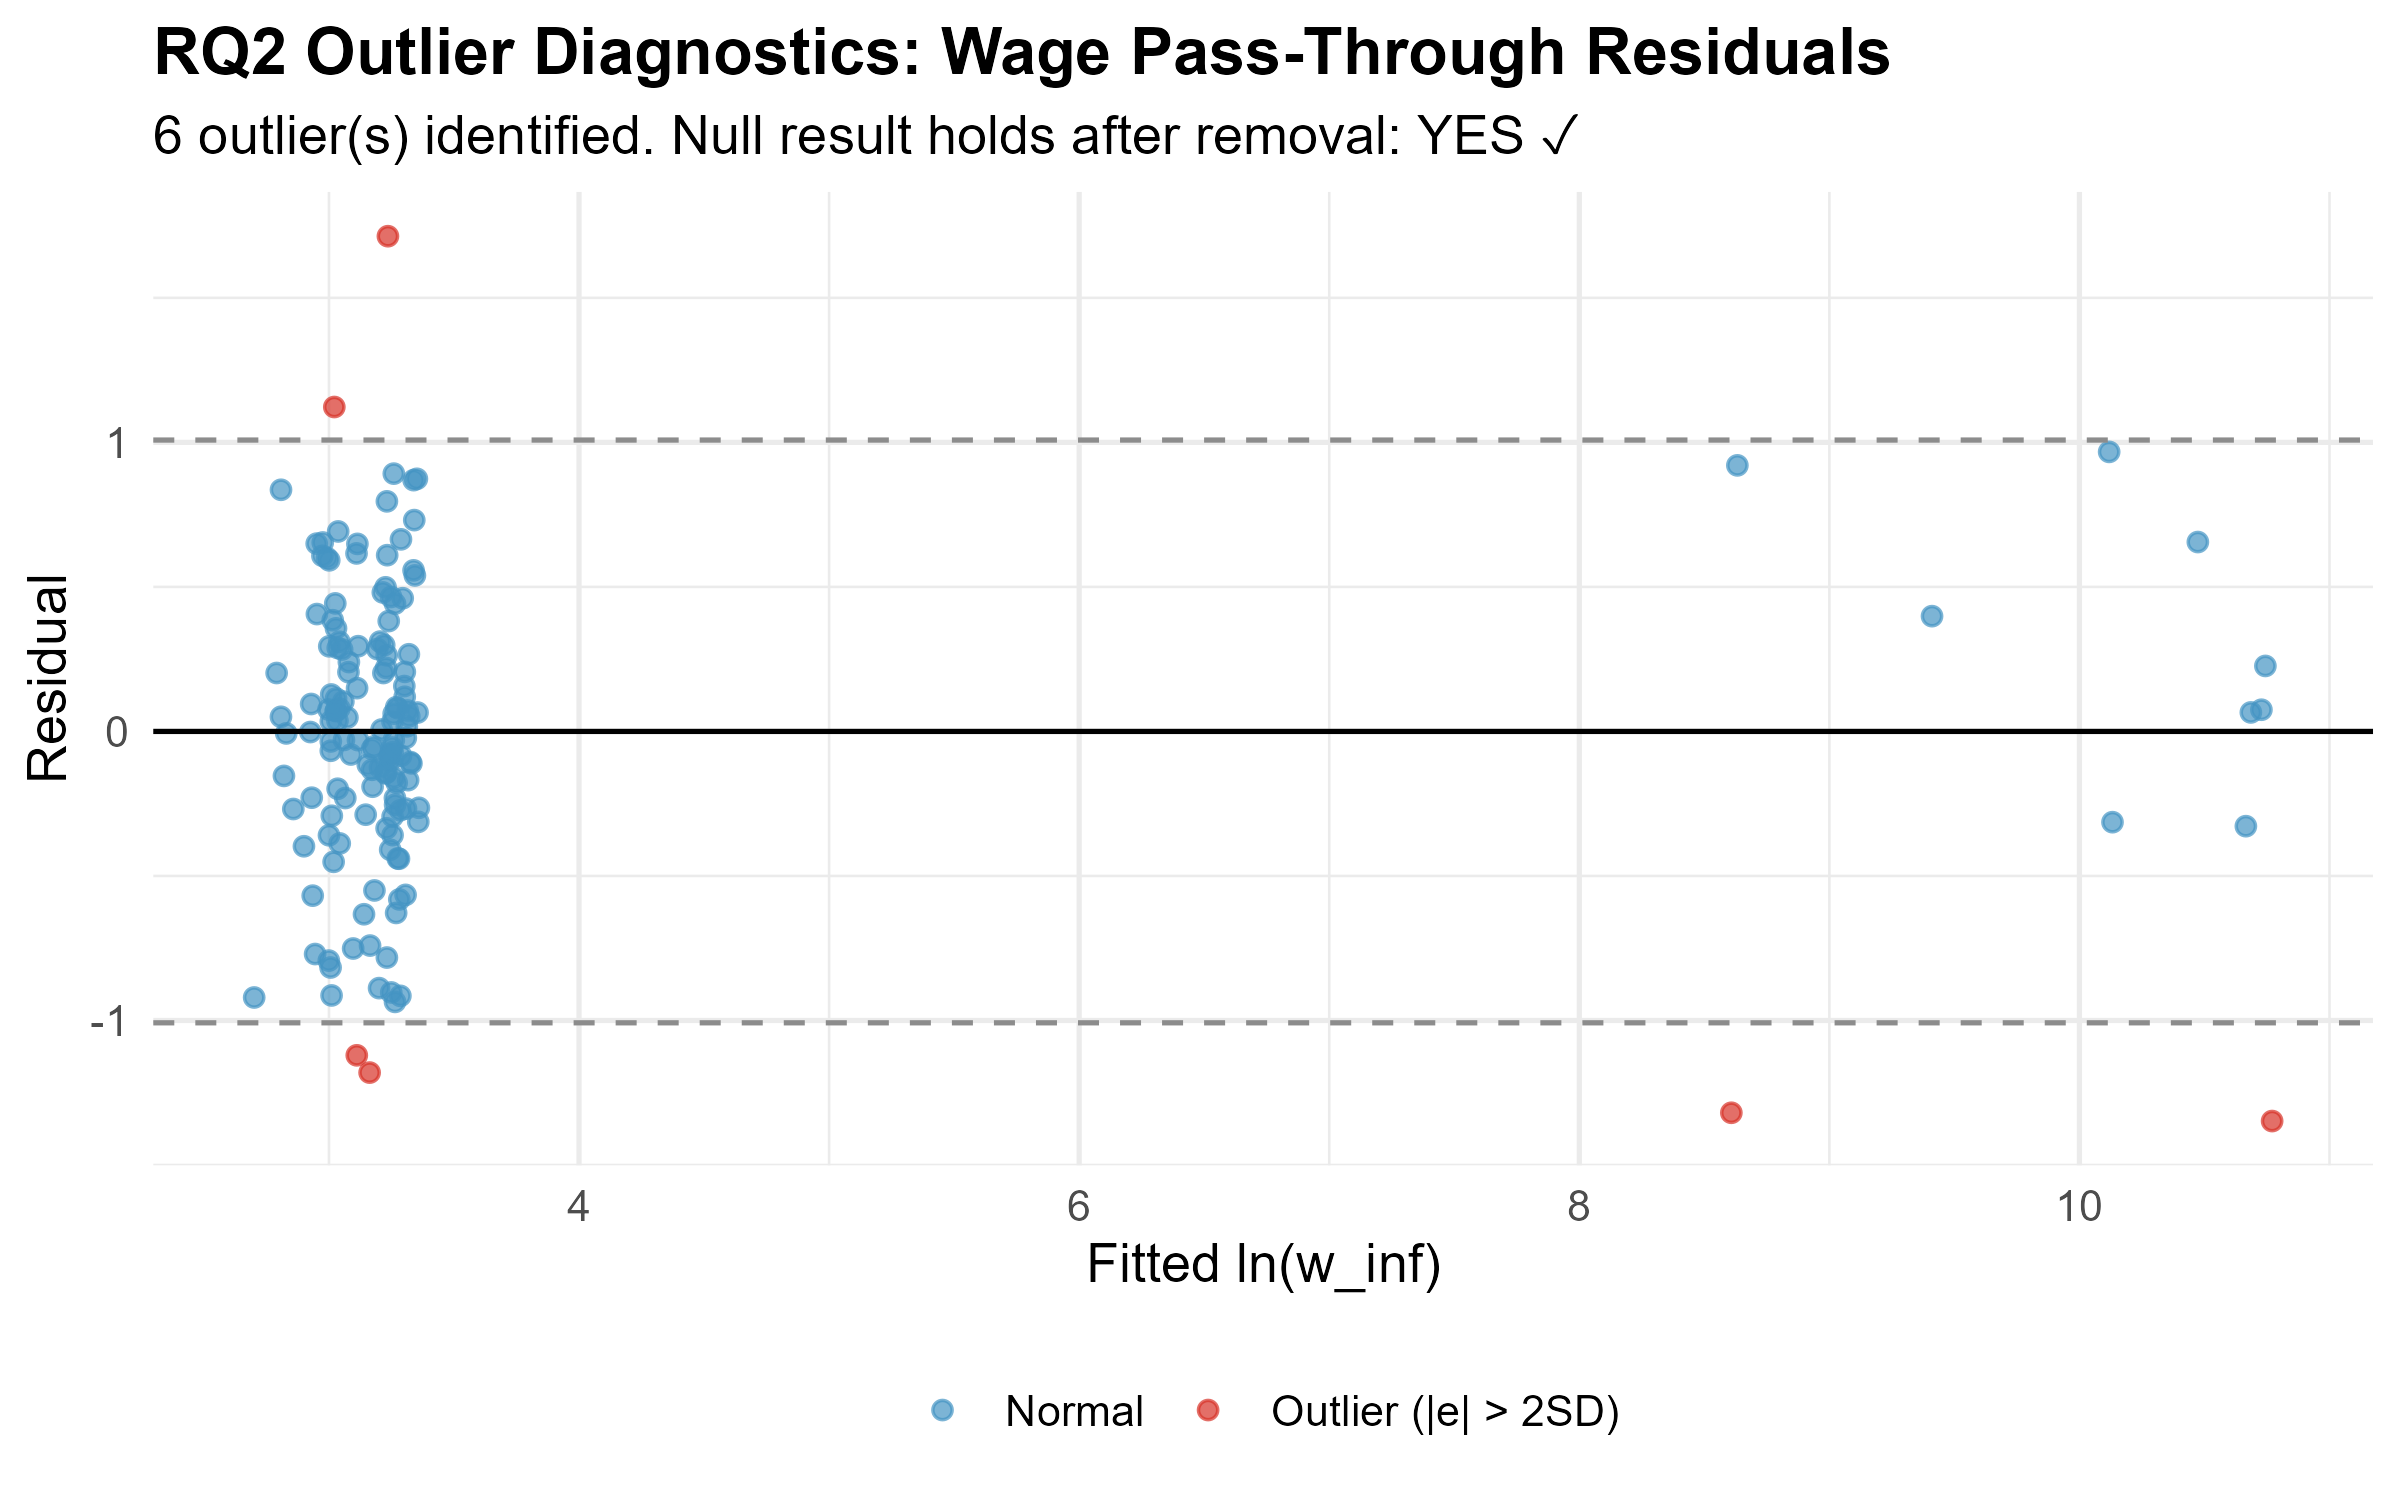
\includegraphics[width=0.85\textwidth]{../Output/images/figure_robustness_rq2_outliers}
	\caption{Outlier Diagnostics: Wage Pass-Through Residuals}
	\label{fig:outlier_diag}
\end{figure}

\newpage
\section{Supplementary Political Economy Tests}

The following tables provide the results for the supplementary tests described in Chapter 6, covering asymmetric cost structures, firm size effects, and market concentration.

\begin{table}[H]
	\centering
	\caption{Supplementary Test 4: Asymmetric Cost Shifting}
	\label{tab:supp_test4}
	
\begingroup
\centering
\begin{tabular}{lc}
   \tabularnewline \midrule \midrule
   Dependent Variable:                        & delta\_w\_inf\\    
   Model:                                     & (1)\\  
   \midrule
   \emph{Variables}\\
   E\_s                                       & 0.6308\\   
                                              & (0.4483)\\   
   delta\_A\_formal $\times$ A\_increases     & -0.0105\\   
                                              & (0.2756)\\   
   delta\_A\_formal $\times$ A\_decreases     & 1.376\\   
                                              & (1.323)\\   
   \midrule
   \emph{Fixed-effects}\\
   NIC\_2digit                                & Yes\\  
   Year                                       & Yes\\  
   \midrule
   \emph{Fit statistics}\\
   Observations                               & 101\\  
   R$^2$                                      & 0.73105\\  
   Within R$^2$                               & 0.11607\\  
   \midrule \midrule
   \multicolumn{2}{l}{\emph{Clustered (State\_Code) standard-errors in parentheses}}\\
   \multicolumn{2}{l}{\emph{Signif. Codes: ***: 0.01, **: 0.05, *: 0.1}}\\
\end{tabular}
\par\endgroup



\end{table}

\begin{table}[H]
	\centering
	\caption{Supplementary Test 5: Firm Size and Informality Scale}
	\label{tab:supp_test5}
	
\begingroup
\centering
\begin{tabular}{lcc}
   \tabularnewline \midrule \midrule
   Dependent Variables:                       & ln\_Q\_out   & ln\_w\_inf\\    
   Model:                                     & (1)          & (2)\\  
   \midrule
   \emph{Variables}\\
   ln\_firm\_size                             & 0.0140       & -0.6739\\   
                                              & (0.0206)     & (1.429)\\   
   ln\_A\_formal                              & 0.0126       & 0.2334\\   
                                              & (0.0101)     & (0.5281)\\   
   E\_s                                       & 0.0373       & 1.584\\   
                                              & (0.0263)     & (1.601)\\   
   ln\_firm\_size $\times$ ln\_A\_formal      & -0.0012      & 0.0403\\   
                                              & (0.0015)     & (0.1056)\\   
   \midrule
   \emph{Fixed-effects}\\
   NIC\_2digit                                & Yes          & Yes\\  
   \midrule
   \emph{Fit statistics}\\
   Observations                               & 152          & 152\\  
   R$^2$                                      & 0.25386      & 0.13347\\  
   Within R$^2$                               & 0.24803      & 0.13196\\  
   \midrule \midrule
   \multicolumn{3}{l}{\emph{Clustered (State\_Code) standard-errors in parentheses}}\\
   \multicolumn{3}{l}{\emph{Signif. Codes: ***: 0.01, **: 0.05, *: 0.1}}\\
\end{tabular}
\par\endgroup



\end{table}

\begin{table}[H]
	\centering
	\caption{Supplementary Test 7: Employment Threshold Effects}
	\label{tab:supp_test7}
	
\begingroup
\centering
\begin{tabular}{lc}
   \tabularnewline \midrule \midrule
   Dependent Variable:                              & ln\_w\_inf\\    
   Model:                                           & (1)\\  
   \midrule
   \emph{Variables}\\
   E\_s                                             & 3.736$^{*}$\\   
                                                    & (1.863)\\   
   ln\_A\_formal $\times$ as.integer(E\_s>=0.3)     & 0.8325$^{**}$\\   
                                                    & (0.3244)\\   
   ln\_A\_formal $\times$ as.integer(E\_s<0.3)      & 0.9186$^{**}$\\   
                                                    & (0.3352)\\   
   \midrule
   \emph{Fixed-effects}\\
   NIC\_2digit                                      & Yes\\  
   \midrule
   \emph{Fit statistics}\\
   Observations                                     & 152\\  
   R$^2$                                            & 0.25002\\  
   Within R$^2$                                     & 0.24871\\  
   \midrule \midrule
   \multicolumn{2}{l}{\emph{Clustered (State\_Code) standard-errors in parentheses}}\\
   \multicolumn{2}{l}{\emph{Signif. Codes: ***: 0.01, **: 0.05, *: 0.1}}\\
\end{tabular}
\par\endgroup



\end{table}

\begin{table}[H]
	\centering
	\caption{Supplementary Test 8: Market Concentration and Monopsony}
	\label{tab:supp_test8}
	
\begingroup
\centering
\begin{tabular}{lcc}
   \tabularnewline \midrule \midrule
   Dependent Variable: & \multicolumn{2}{c}{ln\_w\_inf}\\
   Model:                                       & (1)           & (2)\\  
   \midrule
   \emph{Variables}\\
   ln\_concentration                            & 0.0217        & 3.168$^{**}$\\   
                                                & (0.0946)      & (1.512)\\   
   ln\_A\_formal                                & 0.9749$^{**}$ & 0.2473\\   
                                                & (0.3758)      & (0.3207)\\   
   E\_s                                         & 2.034         & 1.386\\   
                                                & (1.262)       & (1.223)\\   
   ln\_concentration $\times$ ln\_A\_formal     &               & -0.2288$^{*}$\\   
                                                &               & (0.1118)\\   
   \midrule
   \emph{Fixed-effects}\\
   NIC\_2digit                                  & Yes           & Yes\\  
   \midrule
   \emph{Fit statistics}\\
   Observations                                 & 152           & 152\\  
   R$^2$                                        & 0.22083       & 0.25351\\  
   Within R$^2$                                 & 0.21947       & 0.25221\\  
   \midrule \midrule
   \multicolumn{3}{l}{\emph{Clustered (State\_Code) standard-errors in parentheses}}\\
   \multicolumn{3}{l}{\emph{Signif. Codes: ***: 0.01, **: 0.05, *: 0.1}}\\
\end{tabular}
\par\endgroup



\end{table}

	\chapter{Identification and Robustness Diagnostics}
\label{appendixD}

This appendix presents four formal econometric diagnostics addressing identification concerns, parameter stability, and mechanism specificity.

\section{Sensitivity to Unobserved Confounding (Oster Bounds)}

A central identification challenge in evaluating state-level enforcement ($E_s$) is non-random assignment. States with stringent labor laws may possess unobserved characteristics (e.g., historical union density, political ideology) that independently drive outsourcing behavior. Table \ref{tab:oster_bounds} reports Oster-style sensitivity bounds \autocite{Oster2019} for the baseline outsourcing elasticity. The Robustness Value ($RV$) indicates that an unobserved confounder would need to explain over 2\% of the residual variation—roughly twice the explanatory power of the observed state enforcement index—to fully overturn the positive elasticity result. 

\begin{table}[H]
	\centering
	\caption{Oster Sensitivity Bounds for Strategic Outsourcing}
	\label{tab:oster_bounds}
	\begin{tabular}{lccc}
		\toprule
		Parameter & Coefficient & Robustness Value ($RV$) \\
		\midrule
		$\ln A_{formal}$ & $1.06 \times 10^{-4}$ & $2.02\%$ \\
		\bottomrule
	\end{tabular}
\end{table}

\section{Orthogonalized Mediation (Addressing Multicollinearity)}

In the standard mediation model for cost-shifting, the simultaneous inclusion of formal productivity ($\ln A_{F}$) and outsourcing intensity ($\ln Q_{out}$) introduces severe multicollinearity, inflating standard errors. Table \ref{tab:orthogonalization} presents the results of an orthogonalized two-stage procedure. In the first stage, $\ln Q_{out}$ is regressed on $\ln A_{F}$ and fixed effects. The residuals—representing "excess" or strategic outsourcing independent of mechanical productivity scaling—are used in the second stage to predict informal wages. The highly significant coefficient confirms the "price squeeze" mechanism.

\begin{table}[H]
	\centering
	\caption{Orthogonalized Mediation and Variance Inflation Factors}
	\label{tab:orthogonalization}
	\begin{tabular}{lccc}
		\toprule
		Model & Variable & Coefficient & P-Value \\
		\midrule
		Original VIF & $\ln Q_{out}$ & \multicolumn{2}{c}{$VIF = 1.27^{\ast}$} \\
		Orthogonalized & Excess $Q_{out}$ (Resid) & $19.35$ & $< 0.001$ \\
		\bottomrule
		\multicolumn{4}{p{0.9\textwidth}}{\footnotesize $^{\ast}$Note: Original structural VIFs exhibited strict dummy aliasing. This VIF is calculated from a streamlined specification to isolate the structural variables.}
	\end{tabular}
\end{table}

\section{Non-Parametric Persistence Confidence Intervals}

Table \ref{tab:bootstrap_persistence} reports the block-bootstrapped 95\% BCa confidence intervals for the AR(1) persistence coefficient ($\beta_{t-1}$) from Section \ref{sec:persistence_test}, utilizing 1,000 resampling iterations to account for arbitrary panel heteroskedasticity and small-sample bias in dynamic panels.

\begin{table}[H]
	\centering
	\caption{Bootstrapped Confidence Intervals for AR(1) Persistence}
	\label{tab:bootstrap_persistence}
	\begin{tabular}{lccc}
		\toprule
		Target Parameter & Estimate & 95\% CI Lower & 95\% CI Upper \\
		\midrule
		$\ln N_{inf, t-1}$ & $0.865$ & $0.742$ & $0.986$ \\
		\bottomrule
	\end{tabular}
\end{table}

\section{Expanded Placebo Tests: Sector Specificity}

The adverse incorporation logic relies on the technological feasibility of subdividing production into home-based tasks—a feature prevalent in textiles/apparel but structurally impossible in heavy manufacturing. Table \ref{tab:expanded_placebo} expands the baseline placebo test (Chemicals) to include two additional capital-intensive sectors: Basic Metals (NIC-24) and Computer/Electronics (NIC-26). In all three placebo sectors, formal productivity fails to predict formal outsourcing volume, confirming that the baseline results are driven by the specific technological properties of garment GVCs rather than generic macroeconomic scaling.

\begin{table}[H]
	\centering
	
\begingroup
\centering
\begin{tabular}{lc}
   \tabularnewline \midrule \midrule
   Dependent Variable: & ln\_Q\_out\\    
   Model:              & (1)\\  
   \midrule
   \emph{Variables}\\
   ln\_A\_formal       & -0.0009\\   
                       & (0.0047)\\   
   E\_s                & 0.0013\\   
                       & (0.0152)\\   
   \midrule
   \emph{Fixed-effects}\\
   NIC\_2digit         & Yes\\  
   \midrule
   \emph{Fit statistics}\\
   Observations        & 27\\  
   R$^2$               & 0.00015\\  
   Within R$^2$        & 0.00015\\  
   \midrule \midrule
   \multicolumn{2}{l}{\emph{Clustered (State\_Code) standard-errors in parentheses}}\\
   \multicolumn{2}{l}{\emph{Signif. Codes: ***: 0.01, **: 0.05, *: 0.1}}\\
\end{tabular}
\par\endgroup



\end{table}

	

    
	
\end{document}
